%Document vide aux normes de l'École nationale des Chartes
%Dernières modifications E. Rouquette (12/2023)

%%%%%%%%%%%%%%%%%%%%%% PRÉAMBULE


%%%%%%%%%%%%%% partie obligatoire du préambule
\documentclass[a4paper,12pt,twoside]{book}
\usepackage{fontspec}
\usepackage{xunicode}
\usepackage[french]{babel}%on peut préciser d'autres langues.


%%%%%%%%%%%%%%%%%%%%%%%%%%%%%%%%% PACKAGES UTILISÉS

\usepackage{csquotes} % les guillemets français
\usepackage{lettrine} %faire une lettrine (pas obligatoire)

\usepackage[style=enc,sorting=nyt,maxbibnames=10]{biblatex}%charger le style de l'EnC (téléchargeable ici https://ctan.org/pkg/biblatex-enc)
\addbibresource{./bibliographie/bibliographieglobale.bib} %le fichier bibliograhique. Exemple de chemin à partir du dossier où se trouve le document maître:Exemple ./dossierA/fichier.bib
\defbibheading{}{\subsection*{}} %Si l'on veut changer le titre de la/les bibliographie(s)


%%%Faire un ou plusieurs index

\usepackage{imakeidx} %pour faire un ou plusieurs index
\makeindex %commande pour générer l'index


%RAJOUTEZ ICI VOS PACKAGES


\usepackage{chngcntr} %pour gérer la numérotation des figures en continu
\usepackage{tocloft} % pour gérer la table des matières de façon plus fine


%%%%%%%%%%%%%%%%%%%%%%%%%%%%%%%%% CONFIGURATION DE MISE EN PAGE


%%%%%% Les compteurs (sections, subsections, etc)
\renewcommand{\thesection}{\Roman{section}.}%On ne fait apparaître que le numéro de la section
\renewcommand{\thesubsection}{\arabic{subsection}.}%subsection en chiffres arabes
\renewcommand{\thesubsubsection}{\alph{subsubsection}.}%subsubsection en lettres minuscules
%Si l'on veut faire apparaître les subsubsection dans le table des matières (à commenter sinon)
\setcounter{tocdepth}{3}
\setcounter{secnumdepth}{3}  % La subsubsection (profondeur=3 dans la table des matières) apparait numérotée dans la TdM

\renewcommand{\thefigure}{\arabic{figure}} %Numérotation des figures en un seul chiffre arabe

%%%%%  Configurer le document selon les normes de l'école

\usepackage[margin=2.5cm]{geometry} %marges
\usepackage{setspace} % espacement qui permet ensuite de définir un interligne
\onehalfspacing % interligne de 1.5
\setlength\parindent{1cm} % indentation des paragraphes à 1 cm
\setlength{\parskip}{16pt} % espace de 16 points entre les paragraphes

%%%%% Mise en forme des headers (haut de page)

\usepackage{fancyhdr} %package utilisé pour modifier les headers
\pagestyle{fancy} %utiliser ses propres choix de mise en page et non ceux par défaut du package

\setlength\headheight{16pt}%la hauteur des headers
\renewcommand{\sectionmark}[1]{\markright{\small\textit{\thesection~\  #1}}}%Faire apparaître dans les headers les sections en  petit et en italiques
\renewcommand{\sectionmark}[1]{}%Commenter la lign précédetne et mettre celle-ci pour ne pas avoir le titre des sections dans le header
\renewcommand{\chaptermark}[1]{\markboth{\small\chaptername~\thechapter~--\ \textit{#1}}{}}%idem pour les chapitres
%\renewcommand{\chaptermark}[1]{}%Commenter la ligne précédente et mettre celle-ci pour ne pas avoir le titre des chapitres  dans le header



%indiquer des règles d'hyphénation pour des mots précis si besoin
%\begin{hyphenrules}{french}
%	\hyphenation{}
%\end{hyphenrules}


%%%%%%% Package hyperref
% A mettre après les autres appels de packages car redéfinit certaines commandes).

\usepackage[colorlinks=false, hidelinks = true, breaklinks=true, pdfusetitle, pdfsubject ={Mémoire TNAH}, pdfkeywords={les mots-clés}]{hyperref} %
\usepackage[numbered]{bookmark}%va avec hyperref; marche mieux pour les signets. l'option numbered: les signets dans le pdf sont numérotés

% Compléter pdfsubjet et pdfkeywords
%Explication des options de hyperref (modifiables)
% hyperindex=false
% colorlinks=false: pour que le cadre des liens n'apparaisse pas à l'impression
% breaklinks permet d'avoir des liens allant sur pusieurs lignes
%pdfusetitle: utiliser \author et \title pour produire le nom et le titre du pdf
% Hidelinks : permet de faire en sorte que les cadres rouges des liens n'apparaissent pas sur le PDF 

%avec overleaf, utiliser :
%\usepackage[xetex]{hyperref}
%\hypersetup{
	%	pdfauthor = {Prénom Nom},
	%	pdftitle = {titre},
	%	pdfsubject = {sujet},
	%	pdfkeywords = {premier mot-clé} {deuxième mot-clé} {troisième mot-clé} {etc}
	%}



%%%%%%%%%%%%%%%%%%%% Package glossaries

%Exception: il faut le charger APRÈS hyperref
%\usepackage[toc=true]{glossaries}
%\makeglossaries
%avec TexStudio: F9 pour compiler le glossaire (s'il y a aussi un index)

%mettre les entrées du glossaire ici ou les mettre dans un fichier à part que l'on appelle ici par \loadglsentries{nom_du_fichier.tex}

%Structure d'une entrée de glossaire
%\newglossaryentry{}{%
	%	name={},%
	%	description={}
	%}



%%%%%%%%%%%%%%%%%% DÉFINITION DES COMMANDES ET ENVIRONNMENTS



% Commande qui permet de gérer les cas où une citation est issue d'un autre article que celui cité (celles avec un \textit{in})
\newcommand{\citein}[3][]{\footnote{\cite{#2} \textit{in} \cite{#3}#1}}


\counterwithout{figure}{chapter}% pour compter les figures de façon continue 


\setlength{\cftbeforepartskip}{5em}  % Augmenter l'espace entre les parties dans la table des matières



%%%%%%%%%%%%%% INFORMATIONS POUR LA PAGE DE TITRE
\author{Maxime GRIVEAU - M2 TNAH}
\title{La découvrabilité des contenus culturel à l'heure du \textit{big data patrimonial}}

%%%%%%%%%%%%%%%%%%%%%% DOCUMENT
\begin{document}
	\begin{titlepage}
		\begin{center}
			
			\bigskip
			
			\begin{large}				
				ÉCOLE NATIONALE DES CHARTES\\
				UNIVERSITÉ PARIS, SCIENCES \& LETTRES
			\end{large}
			\begin{center}\rule{2cm}{0.02cm}\end{center}
			
			\bigskip
			\bigskip
			\bigskip
			\begin{Large}
				\textbf{Maxime GRIVEAU}\\
			\end{Large}
			%selon le cas
			\begin{normalsize} 
				\textit{diplômé de licence histoire, histoire de l'art et archéologie}
			\end{normalsize}
			
			\bigskip
			\bigskip
			\bigskip
			
			\begin{Huge}
				\textbf{La découvrabilité des contenus culturels à l'heure du \textit{big data patrimonial}}\\
			\end{Huge}
			\bigskip
			\bigskip
			\begin{LARGE}
				\textbf{Cas d'usages à la Radio-télévision Suisse (RTS)}\\
			\end{LARGE}
			
			\bigskip
			\bigskip
			\bigskip
			\begin{large}
			\end{large}
			\vfill
			
			\begin{large}
				Mémoire 
				pour le diplôme de master \\
				\enquote{Technologies numériques appliquées à l'histoire} \\
				\bigskip
				2024
			\end{large}
			
		\end{center}
	\end{titlepage}
	
	\thispagestyle{empty}	
	\cleardoublepage
	
	\frontmatter
	
	\chapter{Résumé}
	\textbf{Résumé} : Ce mémoire, réalisé lors d'un stage à la Radio-Télévision Suisse (RTS) dans le cadre du Master Technologies numériques appliquées à l'histoire (TNAH) de l'École des chartes - PSL, explore la question de la découvrabilité dans le secteur patrimonial. Notion définie comme la \enquote{capacité pour un objet à émerger parmi un vaste ensemble à un utilisateur qui n'en aurait pas fait la demande}\footcite{zotero-263}. Après avoir exploré les enejeux de disponibilité des contenus, leur repérabilité et leur recommandation algorithmique tout en historicisant la notion, le mémoire traite ensuite de l'évolution des interfaces, notamment des catalogues et des visualisations de données, et examine enfin les limites de la notion : écosystème du web, règles institutionnelles et angles morts (accessibilité numérique, explicabilité, et numérique responsable).
	
	\textbf{Abstract}: This thesis, conducted during an internship at Radio-Télévision Suisse (RTS) as part of the Master's program in Digital Technologies Applied to History (TNAH) at the École des chartes - PSL (Paris), focuses on the concept of discoverability in the heritage sector, defined as the \enquote{ability of an object to emerge from a vast array to a user who has not explicitly requested it}. The study explores content availability, findability, and algorithmic recommendation, providing a historical perspective on the notion. It then addresses the evolution of interfaces, particularly catalogs and data visualizations and finally examines the limits of the concept: the web ecosystem, institutional rules and blind spots (digital accessibility, explainability, and responsible digital practices).
	
	\textbf{Mots-clés:} Découvrabilité ; repérabilité ; algorithmes de recommandation ; intelligence artificielle (RAG) ; interfaces ; crowdsourcing ; impact environnemental du numérique ; bulle de filtre ; longue traine.  
	
	\newpage
	
	\textbf{Informations bibliographiques:} Maxime Griveau. La découvrabilité des contenus culturel à l'heure du \textit{big data patrimonial} : cas d'usages à la RTS, mémoire de master \enquote{Technologies numériques appliquées à l'histoire}, dir. Maxime Challon, École nationale des chartes, 2024.
	
	\textit{Ce document est écrit en utilisant l'orthographe réformée, on ne s'étonnera donc pas, par exemple, de l'absence de l'accent circonflexe sur des mots tels que maitre.
		Voir à ce propos : \url{https://www.academie-francaise.fr/sites/academie-francaise.fr/files/rectifications.pdf}}
	\newpage{\pagestyle{empty}\cleardoublepage}
	
	\chapter{Remerciements}
	
	\lettrine{M}es remerciements vont tout d’abord à Janique Sonderegger, documentaliste spécialisée data au service Données \& Archives, qui, pendant toute la durée de mon stage, a su orienter mes réflexions, me fournir des clés de lecture essentielles et les outils adéquats, sans jamais limiter les réflexions et essais que je souhaitais mener.
	
	Je tiens également à remercier Denise Barcella, experte en patrimoine au service Données \& Archives et ancienne enseignante à l’Université de Lausanne, pour ses précieuses indications concernant l’histoire du fonds. Nos discussions m’ont par ailleurs été très utiles pour appréhender, ne serait-ce qu’un peu, la complexité des opérations de numérisation et l’histoire des supports conservés à la RTS.
	
	Ce mémoire doit aussi beaucoup à Maxime Challon, ingénieur data à l’Institut national de l’audiovisuel. Je le remercie pour ses précieux conseils quant à la rédaction du mémoire, mais aussi pour les discussions très fructueuses que nous avons eues. Il a toujours su me guider vers la bonne voie sans jamais m’imposer une direction précise, et a fourni des conseils techniques particulièrement pertinents. Pour les mêmes raisons, je souhaite remercier Emmanuelle Bermès pour ses orientations bibliographiques précieuses et ses conseils lors de la réflexion autour du plan.
	
	Je remercie également tous les collègues avec qui j’ai eu le plaisir d’échanger pour construire l’historique des fonds et de leurs métadonnées, ainsi que sur des sujets extrêmement variés qui m’ont permis de grandir, tant professionnellement que personnellement. Je ne peux tous et toutes les citer ici, mais je tiens à exprimer ma gratitude en particulier à : Laure Meuret, Marie Françoise Guex, Alain Freudiguer, Gabriel Leon, Pietro et Marielle Renzonnico, Didier Bufflier, Martine Cameroni, Sophie Meyer, Soazig Vaucher, Vincent Seriot, Laurent Guimard, Natacha Farina Groux, Louise-Anne Thévoz, Joëlle Albrecht-Glaisen, Gabrielle Frech, Anne-Isabelle Gomez, Floriane Morattel, Rita Crota Ben Henda et, bien sûr, Guy Druey.
	
	Avant de clore ces remerciements, je tiens à remercier Louis Falissard, Maître de conférences en apprentissage profond à l’Université Paris VIII, et Xavier Huet, Administrateur fonctionnel des archives de la métropole de Lille, pour les échanges que nous avons eus, respectivement sur le clustering des contenus et sur la création de la treemap interactive des contenus.
	
	Enfin, je remercie Paul Wang, qui a su me guider, me poser les bonnes questions, et parfois — souvent — me faire douter, toujours pour le meilleur. Je le remercie également pour sa relecture, ainsi que les amis qui ont accepté de prendre ce temps : Jeanne Dugas, Lucile Chatellier-Lang, Alexandra Puillandre, Laurine Roy, Manon Delisle et Maël Jean.
	
	\newpage{\pagestyle{empty}\cleardoublepage}
	
	%%%%%%%%%%%% \bibliographie ici (normes de l'EnC)
	\part*{Bibliographie}
	\printbibliography[keyword=partie1, title={Historique et enjeux}]
	\printbibliography[keyword=partie2, title={Nouvelles interfaces}]
	\printbibliography[keyword=partie3, title={Limites de la notion}]
	
	
	\printbibliography[keyword=dictionnaires, title={Encyclopédies et statistiques}]
	
	
	\chapter{Introduction}	
	 \begin{quote}
	 	\enquote{L’univers (que d’autres appellent la Bibliothèque), se compose d’un nombre indéfini […] de galeries hexagonales, avec au centre de vastes puits d’aération bordés par des balustrades très basses. […] vingt longues étagères, à raison de cinq par côté, couvrent tous les murs moins deux […]. Chacun des murs de chaque hexagone porte cinq étagères ; chaque étagère comprend trente-deux livres, tous de même format ; chaque livre a quatre cent dix pages ; chaque page, quarante lignes, et chaque ligne, environ quatre-vingts caractères noirs \footcite[p. 1]{borges1963}.}
	 \end{quote} 
	
	Dans sa nouvelle, Jorge Luis Borges décrit son « rêve de bibliothèque » : une bibliothèque presque infinie contenant toutes les combinaisons possibles de 23 des lettres de l’alphabet combinées avec l’espace et le point. Rêve car elle contient tous les livres parus, disparus, à paraître ainsi que toutes leurs interprétations, les réfutations des interprétations, dans toutes les langues, mêmes inconnues, mais aussi l’histoire de votre vie, passée, présente, ou future \footcite{marx}.
	
	Mais comme le décrit William Marx dans son cours du collège de France consacré au « rêve de la bibliothèque parfaite », ce rêve tourne vite au cauchemar, celui de la masse, cette bibliothèque n’est pas ordonnée, pas classée, « les nombres s’y multiplient au-delà du raisonnable » \footcite{marx}. Combien de pages contenant d’incompréhensibles suites de caractères vous faudra-t-il consulter pour trouver le récit de votre vie ? Combien de livres devrez-vous ouvrir dans cette bibliothèque finie mais contenant 1.956 × $10^{1834097}$ livres pour y retrouver les œuvres disparues d’Eschyle ? Combien de kilomètres devrez-vous parcourir dans cet espace plus grand que l’univers connu pour y trouver ne serait-ce qu’un livre qui aurait du sens ? La bibliothèque de Babel exprime ainsi le débordement du langage, punition divine infligée aux humains dans le mythe éponyme \footcite{zotero-393}, elle se transforme en cauchemar non pas du fait de sa volumétrie mais par l’absence de classement, par l’impossibilité de retrouver quoi que ce soit dans cette bibliothèque gouvernée par les nombres : \enquote{nombre indéfini de galeries hexagonales contenant chacune 20 étagères contenant chacune 32 livres contenant chacun 410 pages contenant chacune 40 lignes contenant chacune 80 caractères.}
	
	Publiée en 1941, \textit{La bibliothèque de Babel} n’a jamais cessée d’être actuelle, une quantité d’information immense gouvernée par les nombres, écrasants et impossibles à imaginer : on fait assez rapidement le parallèle avec le web, ses Zettaoctets de données \footnote{Un zettaoctet correspond à un million de téraoctets (To) ou un milliard de gigaoctets (Go)}, immense lac dans lequel il est facile de se perdre et où le problème majeur que posait la bibliothèque de Borges, celui de la place prise par ces milliards de milliards de livres n’existe (presque) plus. Ainsi a émergé en 2016 la notion de Découvrabilité \footnote{Nous verrons que si le terme francophone est né en 2016, les questions posées par la découvrabilité ne sont pas neuves} : « capacité qu’a un objet à être repéré parmi un vaste ensemble d’autres contenus, en particulier par une personne qui n’en faisait pas précisément la recherche. » \footcite{zotero-263} qui peut se résumer en trois mots : disponibilité d’abord, repérabilité ensuite, et enfin, recommandation. Les questions posées par la notion, celles de se repérer dans l’immensité documentaire, ne sont pas neuves, Borges les posait déjà en 1941. Ce sont les réponses qui le sont : tout en posant le problème de la masse, le web – et plus largement les technologies de l’information et de la communication – viennent aussi offrir la solution en mettant à notre disposition un arsenal de possibilités de classement que sont les index, moteurs de recherche et autres algorithmes de recommandation.
	
	Cette problématique de la masse se pose aussi de façon exacerbée dans les institutions patrimoniales qui ont (on y reviendra en détails) depuis plusieurs années numérisé, parfois massivement, leurs fonds générant elles aussi une masse qu’il devient difficile d’appréhender. Tel est le cas de la Radio Télévision Suisse (RTS), institution créée en 2011 suite à la fusion de la Télévision Suisse Romande (TSR) et de la Radio Suisse Romande (RSR), réunies en une seule entité d’entreprise (RTS) membre de la Société suisse de Radiodiffusion (SSR) qui en compte trois autres, correspondant aux langues nationales Suisses : la SRF (Schweizer Radio und Fernsehen) pour l’allemand, la RSI (Radiotelevisione svizzera) pour l’italien et la RTR (Radiotelevisiun Svizra Rumantscha) pour le romanche. En une dizaine d’années, la RTS a numérisé la totalité des 680 000 heures d’archives radiophoniques et des 220 000 heures d’archives télévisuelles qu’elle conservait. Une telle masse documentaire pose là aussi la question de la découvrabilité : comment faire en sorte que les utilisateurs, documentalistes, chargés de la valorisation d’un tel fonds s'y retrouvent ? 
	
	Si l’objet du stage effectué à la RTS (pour une durée de quatre mois entre avril et juillet 2024) était au départ de réfléchir à la visualisation des données, un état de l’art réalisé sur le sujet ainsi que des entretiens menés avec une dizaine de personnes utilisatrices du fonds (documentalistes et producteurs de télévision) ont permis de faire émerger un fort besoin d’améliorer la découvrabilité de ce dernier. Les différents chemins parcourus en vue de remplir cet objectif ont donné lieu à l’écriture d’une preuve de concept (POC) sur le domaine (annexée au présent mémoire) mais aussi à une réflexion plus large sur la notion de découvrabilité. Ainsi, au long de ce mémoire nous poserons la question suivante : « Dans un secteur patrimonial où la numérisation a pris une place considérable : quelle importance revêt la notion de découvrabilité et quelles sont ses limites ? » À laquelle nous répondrons en prenant des exemples tirés de notre expérience à la RTS mais aussi d’ailleurs.
	
	Nous commencerons par plonger dans les enjeux autour de la notion de découvrabilité que sont la disponibilité, la repérabilité et la recommandation. Ce sera aussi l’occasion de tenter d’historiciser la découvrabilité : de quoi est-elle le reflet et à quelles questions semble-elle répondre ? Afin d’aborder la repérabilité, et tout au long de ce mémoire, nous nous appuierons sur des éléments vus pendant le stage, ainsi, nous ferons un état des fonds conservés par l’institution ainsi que de leurs métadonnées. Nous évoquerons ensuite la recommandation en passant par l’importance, très patrimoniale, de la notion de sérendipité. La deuxième partie tentera d’aller plus loin en explorant la question des interfaces favorisant la découvrabilité, ces dernières nous semblent en effet capitales dans le cas patrimonial. Ce sera l’occasion de parcourir les transformations des catalogues, l’importance de la visualisation de l’information et ce que nous intitulons les « nouvelles interfaces » et les nouvelles pratiques qui en découlent. Nous terminerons notre mémoire par poser la question des limites et des problématiques, pour cela nous proposerons un état du Web en tant qu’écosystème favorisant ou non la découvrabilité. Nous explorerons ensuite les questions institutionnelles autour de la formation des agents et des réglementations pour terminer ce mémoire par une réflexion sur les angles morts de la notion de découvrabilité que sont l’accessibilité numérique, les enjeux écologiques et ceux d’explicabilité algorithmique.
	\newpage{\pagestyle{empty}\cleardoublepage}
	
	%%%%%%%%%%%%%%%%%Le corps du mémoire
	\mainmatter
	%Trier par dossiers si besoin (front, main,annexes,), se crérer un docuemnt .tex par structure (section ou chapter selon la taille et la pertinence) Exemple de chemin à partir du dossier où se trouve le document maître: ./dossierA/fichier.tex
	
	
	

	
	%Document vide aux normes de l'École nationale des Chartes
%Dernières modifications E. Rouquette (12/2023)

\part{Partie 1 : Historique et enjeux de la notion}
\chapter{Aux origines était la Disponibilité}

\subsection{La nouvelle bibliothèque de Babel : vers un Big data patrimonial}

Depuis plus de vingt ans, les institutions patrimoniales ont massivement numérisé leurs collections. Si l’utopie de recréation d’une « Bibliothèque d’Alexandrie 2.0 » s’est rapidement révélée irréaliste\footcite[p. 20]{bermes2024}, il n’en reste pas moins que le volume de données numérisées est devenu colossal. Cela est encore plus vraie dans le domaine du patrimoine audiovisuel : les institutions occidentales se sont retrouvées, au tournant des années 2000, face à des problématiques de dégradations des supports très importantes, notamment à cause du tristement célèbre « syndrome du vinaigre »\footnote{« Le syndrome du vinaigre est le phénomène de dépolymérisation spontanée qui se produit dans les films pour la photographie ou le cinéma, par dégradation de l’acétate en acide acétique, causant ainsi la détérioration du support des œuvres. » - Wikipédia, Syndrome du vinaigre}. Il a donc fallu numériser ; mais la dégradation des supports n’est pas la seule raison de ces programmes de numérisation massifs, et il nous semble ici intéressant de détailler les autres. En premier lieu, il faut évoquer qu'ils ont eu lieu à une période où la société elle-même se « numérisait » : il y a eu une demande forte de la part des citoyens d’accès à ce qu’ils considéraient comme « leur patrimoine »\footcite{rezzonico2023}; qui plus est — dans le cas de la RTS — la mise à disposition de quelques fragments de la collection avait créé un engouement qui a permis de donner une impulsion au programme de numérisation ; il faut ensuite ajouter à cela un besoin d’accès multiple aux mêmes documents, c’est le cas à la RTS évidemment (plusieurs émissions avaient souvent besoin de réutiliser les mêmes images d’illustration), mais c’est encore plus le cas pour des documents tels que l’État civil, massivement numérisé par les archives départementales. Pour terminer, et c’est loin d’être anodin, il faut ajouter à toutes ces raisons le fait que « c’était possible »\footcite{barcella2024a} : l’arrivée de technologies de stockage de masse (LTO)\footnote{Pour linear tape open, méthode de stockage magnétique permettant de stocker de grands volumes de données de façon plus pérenne que sur disque dur} et de chaînes de numérisation plus rapides et efficaces rendaient la numérisation réalisable et soutenable financièrement. Ce mouvement qui a eu lieu dans les institutions audiovisuelles est un exemple assez extrême : peu d’institutions ont numérisé la totalité de leur patrimoine même si la volonté de le faire n’a pas manqué, elle s’est heurtée à la réalité des métiers et à l’intérêt d’une telle opération\footcite[p. 21]{bermes2024}.

Loin d’être les seules à produire des Données massives\index{Données massives}, les institutions patrimoniales suivent le mouvement initié par les géants du web, et notamment Google qui en 2005 annonce à la foire du livre de Francfort le projet « Ocean » qui vise à numériser intégralement les collections de six puis seize bibliothèques partenaires\footcite{ertzscheid2019}, créant un véritable électrochoc pour les institutions patrimoniales qui intensifient les volumes numérisés\footcite{bermes2024}.

Les données disponibles sur le web, au tournant des années 2010, deviennent donc massives. S’il est très délicat de donner des chiffres sur ce volume, qui de toute manière sont inintelligibles, on estime généralement qu’en 2010 1,2 zettaoctet\footnote{Un zettaoctet correspond à un million de téraoctets (To) ou un milliard de gigaoctets(Go)} ont été produits contre 64 Zo en 2020 et sur ce même volume, environ 2\% seraient conservés soit 3,2 Zo\footcite{zotero-284}. Le secteur patrimonial est loin d’être responsable de cette augmentation, c’est plutôt l’essor du web dit 2.0 : celui des blogs, des réseaux sociaux, de l’interactivité\footcite{zotero-283} décrit en 2009 par Benjamin Bayard dans une phrase qui est devenue célèbre : « L’imprimerie a permis au peuple de lire, internet va lui permettre d’écrire » à qui il faut imputer cette production documentaire massive (suivi de nos jours par les objets connectés). Cette surabondance documentaire sans précédent pose évidemment des questions de découvrabilité, et plus encore de recherchabilité. De fait, dès 2007, un article intitulé « The discoverability of the web »\footcite{dasgupta2007} pose la question du pourcentage de pages renvoyées par un moteur de recherche sur un sujet donné par rapport aux sources utiles : face à la masse grandissante de contenus sur le web, comment garantir la pertinence et l’efficacité des moteurs de recherche ? C’est bien là un signe que l’enjeu de découvrabilité n’est pas intrinsèque au secteur public et patrimonial.

Dans tous les cas, les volumes de données sont tels qu’on peut parler, dans notre cas de Big data\index{Big data} patrimonial\index{Big data\index{Big data} patrimonial|see{Big data\index{Big data}}} : 10 millions de documents sur Gallica, la bibliothèque numérique de la Bibliothèque nationale de France\footcite{zotero-281}, 53 millions sur Européana\footcite{zotero-280}, portail\index{Portail} européen regroupant les bibliothèques numériques du continent, 1 million d’heures de programmes numérisés à la RTS\footcite{sonderegger2024}, 28 millions à l’Institut national de l’audiovisuel (INA) totalisant 80 pétaoctets de données\footcite{alquier2024}. Les volumes sont tels qu’il devient totalement impossible pour l’humain d’appréhender les collections numérisées de façon globale (rendant leur consultation fastidieuse), qui plus est dans un contexte où les institutions patrimoniales sont loin d’être les seules à proposer du contenu en ligne : la bataille est rude pour capter l’attention des utilisateurs.

\subsection{Quand la \enquote{Fatigue muséale\index{Fatigue muséale}} rencontre \enquote{l'économie de l'attention}}

En 1916, Benjamin Ives Gilman posait le concept de Fatigue muséale\index{Fatigue muséale}\footcite{gilman_museum_1916}, fatigue ressentie par le visiteur d’un musée explorant une vaste collection. S’il est vrai que l’article originel est plus focalisé sur la posture du visiteur : souvent obligé de s’accroupir, de se baisser, pour regarder des objets parfois de tailles très réduites dans des vitrines aux reflets problématiques ; on peut étendre cette notion à une fatigue mentale dans laquelle le visiteur serait plongé par une trop grande abondance d’informations et d’objets riches à la fois visuellement et sémantiquement et par le manque de visibilité globale d’une collection : rendant sa compréhension épuisante\footcite[pp. 1-2]{windhager2018a}. 

D’une part, comme noté plus haut, on a des collections patrimoniales massivement mises en ligne et qui génèrent une Fatigue muséale\index{Fatigue muséale}, car impossibles à appréhender dans leur ensemble et de l’autre, une ressource qui se raréfie : l’attention. Qui est placée au centre du modèle économique du web si bien qu’on vient à parler d’une « Économie de l’attention\index{Économie de l’attention} » en reprenant le concept posé par Herbert Simon en 1971 et bien étudié en France par Yves Citton qui le définit comme un modèle fondé, non pas sur la rareté de l’offre face à la demande, mais tout à fait le contraire c’est-à-dire que la chose rare est ici la capacité de réception du public, son attention\footcite[Citton Yves, \enquote{pour une écologie de l’attention}, Paris, Seuil, 2014, p. 16 \textit{in}]{durand2016} : donc dans un monde où l’offre est pléthorique, c’est ici la demande qui est précieuse. Cela constitue une véritable rupture pour les politiques culturelles et surtout en France, et il nous semble important de revenir sur cela en détail. 

Depuis la création du ministère de la Culture en 1959, la politique mise en œuvre était celle de l’offre ; André Malraux partait en effet du postulat que la médiation était inutile, car il considérait en effet que les œuvres étaient performatives et permettaient à leur regardeur de se transcender\footcite[§3]{godin2011} et donc que la Politique culturelle\index{Politique culturelle} devait être tournée vers l’offre uniquement, sans médiation\footcite{pellegrin2022}. En témoigne une politique de l’offre, matérialisée par la création dans chaque département des maisons de la culture pour que, selon André Malraux : « n’importe quel enfant de seize ans, si pauvre soit-il, puisse avoir un véritable contact avec son patrimoine national et avec la gloire de l’esprit de l’humanité »\footcite[Entrée \enquote{maison de la culture}]{waresquiel2001}. Si l’arrivée au pouvoir de la gauche en 1981 et de Jack Lang au ministère de la Culture fait changer les politiques culturelles notamment du point de vue de la création qui s’ouvre aux cultures du monde et aux cultures dites alternatives (fondation du festival international de théâtre de rue d’Aurillac en 1986)\footcite{waresquiel2001} on voit poindre la remise en cause d’un art performatif ne nécessitant pas de médiation avec la mise en place de l’EAC (éducation artistique et culturelle). Le tournant majeur se situe vers 2010, cela coïncide d’ailleurs avec le phénomène de « Big data\index{Big data} patrimonial\index{Big data\index{Big data} patrimonial|see{Big data\index{Big data}}} » décrit plus haut, Frédéric Mitterrand, récemment nommé rue de Valois, veut rompre avec la politique de la « culture pour tous », fondée sur l’offre et avance l’idée d’une « culture pour chacun »\footcite{2010} qui se voudrait plus volontaire en allant vers les personnes dites éloignées de la culture. Si à l’époque son discours avait été très fortement décrié par les acteurs culturels, force est de constater, comme le relève Claude Poissenot\footcite{zotero-269}, que plusieurs actions ont été mises en œuvre dans ce sens ces dernières années, et notamment le Pass Culture, dont l’objectif est de donner à voir aux jeunes une grande variété de contenus culturels en leur proposant d’en choisir un certain nombre via des crédits (tout en conservant une certaine hiérarchie) : l’argent public est donc placé du côté de la demande, pour la stimuler et non plus de l’offre et c’est un changement fondamental.

Le tournant de l’année 2010 fait donc émerger deux problèmes : celui d’une surabondance de l’offre et celui, concomitant, d’une raréfaction de la demande que des collections massives fatiguent rapidement. C’est à ces deux problématiques que semble vouloir répondre la notion de découvrabilité que nous tâcherons d’historiciser dans la prochaine partie.


\subsection{La naissance de la découvrabilité}

Il est difficile de donner une date précise à la naissance de la notion de découvrabilité tant que les questions qu’elle pose sont anciennes : comment naviguer dans le milliard de documents d’archives conservées avant la Révolution en France ?\footcite{poncet2022} Que répondre à Michelet qui, en 1869, se plaignait d’être « inondé de journaux, de romans et d’un déluge de papier » ?\footcite[p. 47]{bermes2024} Il nous faut en revanche noter qu’elle s’est cristallisée au tournant des années 2010, moment où les institutions patrimoniales, et plus généralement le web, voient leur volume documentaire décupler, on l’a vu. Ce qui change fondamentalement ici, c’est que les technologies de l’information et de la communication, en posant le problème de la masse, laissent aussi entrevoir une solution au travers de la notion de découvrabilité qui découle directement de celle de la crainte d’une perte de diversité culturelle accentuée par le web et ses effets de viralité et de Bulle de filtre\index{Bulle de filtre} (sur lesquels nous reviendrons). Ainsi, en 2005, l’UNESCO publie une déclaration sur la diversité culturelle qui exprime la crainte que les technologies de l’information et de la communication viennent renforcer un déséquilibre de visibilité des cultures minoritaires par rapport aux cultures déjà majoritaires :

\begin{quote}
	« Constatant que les processus de mondialisation, facilités par l’évolution rapide des technologies de l’information et de la communication, s’ils créent les conditions inédites d’une interaction renforcée entre les cultures, représentent aussi un défi pour la diversité culturelle, notamment au regard des risques de déséquilibres entre pays riches et pays pauvres, »\footcite{zotero-266}
\end{quote}

Au moment où les pouvoirs publics constatent d’une part l’échec partiel de la politique de l’offre et envisagent de se tourner vers une politique de la demande, et d’autre part reconnaissent la difficulté de se démarquer en ligne au milieu d’une multitude de contenus, il devient essentiel pour eux d’assurer leur visibilité. Ce n’est donc pas un hasard si l’évènement considéré comme fondateur de la notion de découvrabilité s’est tenu pendant la même décennie. En l’occurrence, en 2016 au Canada, et a eu pour sous-titre « le contenu à l’ère de l’abondance ». Il a été organisé par Le Conseil de la radiodiffusion et des télécommunications canadiennes (CRTC) et l’Office national du film du Canada (ONF)\footcite[Ironie du sort, le site orignellement lié au sommet est indisponible mais a été sauvegardé sur Internet Archive]{conseildelaradiodiffusionetdestelecommunicationscanadiennescrtcetlofficenationaldufilmducanadaonf2016}, illustrant le lien — dans les politiques culturelles — entre découvrabilité et contenus audiovisuels.

En France, si la pandémie a clairement mis en avant la notion de découvrabilité, l’élément activateur semble être la grande enquête sur les pratiques culturelles de 2018 qui notait un « essor considérable des pratiques culturelles numériques » et qui consacrait dans le même temps une fréquentation des lieux culturels en hausse « surtout après [l’âge de] 40 ans » et une montée en puissance dans la population la plus jeune des pratiques culturelles numériques, quelles qu’elles soient : écoute de musique, jeux vidéos, mais aussi visionnage de films. Ainsi, la consommation quotidienne de télévision et de vidéos est en baisse pour toutes les catégories d’âges si l’on s’intéresse uniquement au linéaire,\footnote{La télévision/radio dite linéaire est celle qui est suivie en direct en tant que flux, elle se différencie de la consommation à la demande où le téléspectateur/auditeur regarde/écoute les programmes selon son choix, en ligne} mais en hausse si on y ajoute la consommation de vidéos en ligne.\footcite[p. 24]{2020b} D’où, probablement, le projet de lancement de la mission sur la découvrabilité en avril 2019 (planifiée avant la pandémie), qui rend un rapport sur la notion en novembre 2020.\footcite{zotero-263} C’est effectivement un moment où l’inquiétude pour les institutions culturelles de ne pas retrouver leur public du fait de changements d’habitudes (télétravail, digitalisation), est très présente et où les confinements successifs déplacent les pratiques culturelles vers le web. Prenons l’exemple des salles de cinéma, dont la fréquentation avait chuté à un niveau inférieur à 40\% de ce qu’elle était en 2019 en 2022 à la fin des mesures liées à la crise sanitaire ; la crainte de la perte du public était très présente et il était essentiel que les salles de cinéma et leurs contenus (notamment le cinéma francophone) restent visibles alors que les pratiques culturelles avaient été déplacées en ligne.\footcite[§1 et §2]{muller2022} Même s’il faut aujourd’hui nuancer les craintes exprimées en 2022 ; l’année 2023 a montré que les salles noires regagnaient en vitalité pour atteindre un niveau de recettes presque équivalent à celui d’avant la crise sanitaire.\footcite{2024m} Les pratiques culturelles en ligne ont pris une importance capitale et il fallait pour les pouvoirs publics disposer d’outils pour promouvoir « les contenus culturels francophones ».

On l’a vu, l’émergence de la notion de découvrabilité découle d’un long processus et se veut une réponse aux enjeux de surabondance des contenus sur le web dans un contexte attentionnel raréfié. Nous avons décrit le premier enjeu du triptyque de la découvrabilité : la disponibilité\index{Disponibilité}, et avant de passer au deuxième, la repérabilité\index{Repérabilité}, il nous faut décrire le fonds conservé à la RTS, ce dernier exemplifie, en effet, très bien les processus mis en oeuvre par les institutions patrimoniales en matière de disponibilté. 

\chapter{Un fonds massif aux métadonnées complexes : état des fonds conservés par la Radio-Télévision Suisse (RTS)}

Afin de pouvoir y faire référence dans cette partie et dans les suivantes, il nous semble opportun de décrire de façon détaillée l’histoire du fonds de la RTS et de ses métadonnées. Nous nous appuierons ensuite, quand nous le jugerons pertinent, sur cette description pour étayer notre propos par des exemples tirés des pratiques locales et des expérimentations menées pendant notre stage. 

\subsection{Un \enquote{dépot légal} audiovisuel en Suisse ?}


Si en France, depuis 1992, l’INA (Institut national de l’audiovisuel) a la charge d’un dépôt légal intégral des flux audiovisuels, ce n’est pas le cas en Suisse, malgré le fait que l’article 21 de la loi fédérale sur la radio et la télévision (LRTV) soit intitulé « dépôt légal »\footcite{zotero-260}. En effet, le décret d’application (Ordonnance sur la radio et la télévision, ORTV) dans sa section « dépôt légal » réduit le champ à la conservation durable des émissions. Il est ici important de différencier les programmes, qui sont un ensemble d’émissions rassemblées (on parle de « grille des programmes »), et les émissions, qui sont donc un sous-ensemble contenu dans un programme\footnote{« L'emploi du mot programme comme synonyme d'émission est impropre, un programme étant une grille regroupant plusieurs émissions. » - Wikipédia, émission, consulté le 18/07/2024}. Si l’on s’en tient à la définition de l’ORTV, la RTS est tenue de conserver uniquement les émissions, éliminant de facto tout ce qui n’est pas inclus dedans, par exemple les publicités ou encore la météo. En revanche, la RTS est tenue de conserver depuis 1984, pendant quatre mois, tous les programmes diffusés à l’antenne pour vérification par l’Autorité indépendante d’examen des plaintes en matière de radiotélévision (AIEP).

Maintenant que le cadre légal, de jure, est posé, plongeons dans les fonds, de facto : comprendre leur histoire et celle de leurs métadonnées est indispensable pour cerner les enjeux autour de leur découvrabilité.

\subsection{Le fonds radio et ses métadonnées}
\subsubsection{L'origine de la Radiodiffusion en Suisse romande}

En 1922, un émetteur radio fut installé — et quelle poésie — au « Champ-de-l’Air » près de Lausanne, initialement destiné à l’aviation pour la ligne Lausanne-Paris, fournissant des messages météorologiques et des avis de départ aux vols. Roland Pièce, pionnier de la radiodiffusion en Suisse, raconte : « Pour faire passer agréablement le voyage aux passagers, j’ai déjà eu l’idée de leur transmettre des disques de gramophones »\footcite{1939}. La première émission eut lieu en octobre 1922, lors de l’inauguration de la station du Champ-de-l’Air, où un concert fut organisé pour les autorités présentes. Après les discours, les hymnes retentirent avec la particularité que l’orchestre était diffusé, tel un Chant dans l’air, sur des haut-parleurs, marquant ainsi la naissance de la radiodiffusion en Suisse romande\footcite{1939}. La Suisse fait donc partie des pionniers de la radiodiffusion en Europe dès 1922, aux côtés de la France (émetteur de la tour Eiffel), de la BBC et de nombreuses initiatives aux États-Unis\footcite{2022a}. 
En 1931, l’inauguration de l’émetteur de Sottens a marqué une étape cruciale dans l’histoire de la radiodiffusion en Suisse romande\footcite{zotero-256}. La même année, le Conseil fédéral s’empare du sujet et crée la SSR (Société Suisse de Radiodiffusion et Télévision) en tant qu’organisation faitière des chaines et émetteurs locaux, c’est le début d’une diffusion plus régulière des émissions. À cette époque, les deux principales stations, Radio Genève et Radio Lausanne (qui fusionneront en 1964), devaient se partager les créneaux horaires\footcite{2022a}.

\subsubsection{Histoire du fonds et de ses lacunes}


Aux prémices de la radio (1922 en Suisse romande), les émissions étaient diffusées en direct sans conservation de documents. Ce n’est qu’au cours des années 1930 (les premières diffusions ont lieu en 1921), avec le développement de la technologie des disques 78T à gravure directe, qu’il est devenu possible d’enregistrer les émissions, non pas pour constituer une archive, un patrimoine, mais pour permettre leur rediffusion\footcite[p. 26]{prongue2009}.

Dans les années 1950, la bande magnétique supplante progressivement les disques 78T en tant que principal support d’enregistrement. Ce format a été utilisé jusqu’à la fin des années 1990, avant l’adoption des supports numériques tels que les CD-R et les disques magnétooptiques (MOD). À partir de 2003, la production et l’archivage des programmes radiophoniques se sont entièrement numérisés\footcite[p. 27]{prongue2009}, ce qui ne veut pas dire que tout est conservé, seuls 20 à 30 \% des documents sont alors archivés et documentés, souvent à la demande des directeurs adjoints de la rédaction ou des producteurs ou suivant des critères tels que : « Dans 25 ans on en parle », « Suissitude », « commercialisable », « rare », « vie de tous les jours », « déclarations importantes », « illustrations »…\footcite{meuret2024}.

Les fonds sont le reflet de l’histoire de la radiodiffusion en Suisse romande, marquée par une diffusion sur deux sites principaux, Lausanne et Genève. Jusqu’en 1998, les archives étaient constituées séparément par les radios d’alors : Radio-Lausanne et Radio-Genève (réunies en 1964 sous le nom de Radio Suisse Romande [RSR]). Ce n’est qu’après la réunification des services de documentation des deux studios à Lausanne en 1998 que le fonds a été unifié. Sa volumétrie est aujourd’hui de 680 000 heures\footcite{sonderegger2024}.

\subsubsection{La numérisation du fonds radiophonique}
\textit{On se référera à l’annexe A pour une chronologie détaillée des supports conservés par la RTS}

Comme le fonds télévisuel, celui de la radio a été numérisé au tournant des années 2000, d’abord les 78 tours, car leur dégradation faisait craindre des pertes irrémédiables, à partir de 1995 (copiés sur CDR puis numérisés) ; puis les bandes magnétiques dans le cadre du projet NumA (numérisation accélérée) en 2006, qui visait à numériser 25 \% du fonds en 3 ans\footcite[p. 20]{prongue2009}. Deux autres projets ont vu le jour sous l’impulsion d’institutions souhaitant conserver « leurs » archives : l’Orchestre de la Suisse romande, le Canton de Fribourg (projet Patrimoine sonore fribourgeois) et le canton du Jura (projet Jura)\footnote{Eadem.}.

À l’heure actuelle, l’immense majorité du fonds a été numérisé grâce à des partenariats avec l’association MemoriAV (association fondée en 1995 pour la préservation du patrimoine audiovisuel suisse)\footcite{zotero-254} et de la fondation Fonsart (fondée en 2005 par la RTS)\footcite{freudiguer2024} ; en revanche l’intégration des métadonnées dans les outils documentaires reste lacunaire, ce qui fait que les anciennes cartothèques sont parfois encore utiles pour certaines parties du fonds et périodes et qu’une bonne connaissance du fonds est indispensable pour s’y retrouver.


\subsubsection{Métadonnées du fonds radiophonique}

L’une des difficultés concernant le fonds radiophonique est l’extrême hétérogénéité de ses métadonnées. Ces dernières sont le reflet des multiples campagnes de numérisation (on l’a vu), des histoires « séparées » de Radio Genève et Radio Lausanne jusqu’en 1998 et enfin, des changements d’outils et de pratiques documentaires. On tâchera d’en faire une description chronologique et d’expliquer les diverses migrations à chaque fois qu’elles sont intervenues afin de documenter au mieux les incohérences et lacunes éventuelles.

Commençons par les cartothèques, qui étaient à l’origine au nombre de deux, une pour chacune des radios. Les deux étaient séparées entre les disques commerciaux et les enregistrements d’émissions sur bandes magnétiques (parlé et musique)\footcite[pp. 34-37]{prongue2009}. Poursuivons avec les bases de données Ge-Arch et La-Arch, ce sont les inventaires des fonds 78 tours des deux radios romandes réalisés au moment des numérisations évoquées\footcite[p. 33]{prongue2009}.

Toutes numérisées au cours des années et réparties entre différentes bases de données hébergées localement, il faudra attendre 2003 et la mise en place de SIRANAU (Système Intégré Radiophonique d’Archivage Numérique Audio) pour que les métadonnées soient rassemblées au sein du même outil, qui permet en outre de jouer directement les archives numérisées. Ce logiciel contient donc : l’ensemble des métadonnées et données du fonds radiophonique (elles ont été ajoutées au fur et à mesure des numérisations)\footcite[p. 37]{prongue2009}. Ce n’est pas sans poser un problème de cohérence puisque le niveau hiérarchique le plus haut dans SIRANAU est le programme, qu’il est parfois très difficile de relier à la matérialité des objets : notamment des 78 tours à gravure directe qui étaient utilisés par paire. On enregistrait sur l’un, quand une face se terminait, on passait à l’autre, puis on tournait le premier : et ainsi de suite. Ce qui a pour conséquence d’avoir des programmes « éclatés » sur plusieurs supports et avec parfois une face contenant un morceau d’un programme et, sur l’autre, un programme tout à fait différent.

Avec la fusion en 2011 de la RSR (Radio suisse romande) et de la TSR (Télévision Suisse romande), un projet de fusion entre les outils documentaires de la Télévision (Gico) et de la Radio (SIRANAU) a été lancé, il devrait voir le jour prochainement.

\subsection{Le fonds télévisuel et ses métadonnées}

\subsubsection{Histoire du fonds et de ses lacunes}
\textit{On se référerra à l'annexe A pour une chronologie détaillée des supports conservés par la RTS}

Le fonds télévisuel de la RTS commence avec les débuts de la diffusion en 1954. Aujourd’hui, il totalise environ 220 000 heures d’enregistrements, soit directement numériques (depuis le passage au support LTO en 2008), soit issus de la numérisation des fonds réalisée entre 2004 et 2014. Ce fonds, loin d’être monolithique, reflète l’histoire technique, institutionnelle et humaine de la RTS. Une analyse détaillée est essentielle pour comprendre son évolution et ses éventuelles lacunes, tant au niveau du contenu qu’au niveau des métadonnées.

Plusieurs facteurs peuvent expliquer la non-conservation de certaines émissions :

\textbf{Techniques :}

Les couts de stockage étaient très élevés avant la généralisation des cassettes Betacam en 1987, ce qui entrainait le réenregistrement sur des bandes avec effacement des anciennes émissions. L’archivage était en conséquence, cher et réduit à l’essentiel. Enfin, l’évolution rapide des supports de stockage (14 supports différents depuis la création de la RTS) rendait difficile la lecture des supports anciens.\footcite{barcella2024a}

\textbf{Organisationnels :}

Le service Données et archives (d’abord Téléthèque puis Documentation et archives) était initialement un service de documentation, comme en témoigne la première « Directive concernant l’archivage des émissions à la RTSR » du 1er avril 1981. Celle-ci établissait des critères de sélection basés sur cinq fonctions : vente/échange d’émissions, réutilisation, recours au contenu informatif, mise à disposition de copies à des tiers, et conservation pendant les quatre mois légaux (voir plus haut) ; des critères documentaires et non patrimoniaux. La conservation de certaines émissions a ainsi été jugée peu utile, notamment les émissions pour enfants, le sport, et les émissions de divertissement (jeux). Aussi, pour certains documents, on ne conserve que « clean feed » (sans son et sans incrustations à l’écran), car l’objectif de la conservation était la réutilisation des images.
Par ailleurs, avant 1959, la RTS ne disposait pas d’appareil de captation des émissions en direct (kinescope), et dépendait donc de la SRF à Zurich pour l’enregistrement. Certaines archives sont en conséquence conservées à la SRF, comme le Téléjournal diffusé depuis Zurich jusqu’en 1981 avec un commentaire romand. Enfin, le flux télévisuel n’a jamais été conservé, seulement les émissions, ce qui rend rare la conservation de séquences comme les publicités ou les passages d’antenne par des speakerines.\footcite{barcella2024a}

\textbf{Humains :}

Les facteurs sont ici multiples : oublis d’enclenchement des magnétoscopes pour l’enregistrement des émissions ; documents prêtés et non rendus, ou mal conservés (proche des fenêtres !). Notons que l’informatisation des années 1980 a permis une meilleure préservation des archives, les commandes et la gestion des cassettes étant dès lors supervisées par des documentalistes qui assuraient leur retour et leur préservation systématique. La notion de « patrimoine audiovisuel » n’est apparue que dans les années 2000, activée notamment par les anniversaires de la télévision en 2004, moment coïncidant avec l’initiative de numérisation massive du fonds.\footcite{barcella2024a}

\subsubsection{La numérisation du fonds télévisuel}

Entre 2004 et 2014, l’immense majorité des 120 000 cassettes, représentant la majorité des supports physiques conservés, a été numérisée (90\%). Cette initiative peut s’expliquer par plusieurs aspects. Tout d’abord, la digitalisation de la société a entrainé une demande forte de la part des citoyens d’accès à leurs archives. Une petite partie du fonds avait déjà été numérisée et mise en ligne, et son succès avait été fulgurant\footcite{rezzonico2023}.

Ensuite, le vieillissement des supports a été un facteur crucial : les films ont été touchés par le syndrome du vinaigre, qui a fini par se propager et contaminer les cassettes stockées dans le même dépôt. De plus, les appareils de lecture devenaient rapidement obsolètes. Les besoins documentaires étaient également importants ; il arrivait souvent que plusieurs émissions nécessitent le même document en même temps, notamment lors de commémorations. La digitalisation permettait alors de multiplier les canaux de diffusion.\footcite{barcella2024a}

La conscience accrue de cette problématique et de l’importance du patrimoine audiovisuel était partagée par Gilles Marchand, directeur de l’époque. De plus, l’engagement de Didier Bufflier, expert en restauration, a mis en lumière les problèmes de conservation importants. Enfin, les évolutions technologiques, notamment avec l’arrivée des LTO, ont rendu possible le stockage à moindres coûts des documents numérisés.\footcite{barcella2024a}

Avec la fin du projet de numérisation en 2014, la direction a souhaité jeter les supports devenus inutiles. Cependant, l’association MemoriAV a alarmé la RTS, soulignant qu’en l’absence de contrôle qualité, jeter les supports serait une erreur. Ainsi, un contrôle qualité a été lancé, assisté par l’Intelligence artificielle\index{Intelligence artificielle|see{IA\index{IA}}} qui détecte les potentielles erreurs, ensuite vérifiées manuellement par des civilistes (le service civil est l'alternative offerte aux hommes suisse ne désirant pas faire leur service militaire).\footcite{barcella2024a}

Toutefois, tout n’a pas été numérisé à cette époque. Il reste entre 5 et 10 \% des supports à numériser, principalement le sport, car la RTS n’est que rarement propriétaire des images diffusées, comme c’est le cas pour le Tour de France, et ce patrimoine est mal considéré. Par ailleurs, les supports difficiles à numériser sont restés de côté, étant les plus problématiques et mal conservés. Certaines cassettes Betacam ont été contaminées par le vinaigre (qui touchait le fonds des films 16 mm) et d’autres Betacam ont vu leur liant magnétique mal vieillir (sticky shed syndrome). Enfin, certaines cassettes étaient en prêt ou perdues lors de l’opération, bien que beaucoup aient été retrouvées lors des déménagements de la tour pour cause de travaux.\footcite{barcella2024a}

\subsubsection{Métadonnées du fonds télévisuel}

Depuis la création du fonds, celui-ci était constitué de fiches catalographiques. L’informatisation a débuté dans les années 1980 avec le passage au logiciel « Gesima » (pour Gestion des images), dont le nom illustre bien l’objectif : retrouver aisément des archives afin de pouvoir les réutiliser pour illustrer un nouveau sujet. Ce logiciel (et son successeur Gesima2 qui sera remplacé en 2014) fonctionnait selon le principe de la « méthode point-trait » héritée des fiches catalographiques qui consiste à séparer les différents champs par des signes de ponctuation particuliers, le programme se charge ensuite de ventiler dans les différents champs les informations saisies.\footcite{barcella2024a}

En 2014, la RTS est passée au logiciel GICO « Gestion des images et des contenus » : le mapping\footnote{Le mapping désigne le processus d'associer ou de convertir des données d'un format ou d'une structure en un autre.} réalisé alors a utilisé les règles de ponctuation afin de ventiler dans les nouveaux champs les anciens contenus. Par exemple, avant Gico, les différents sujets d’une émission étaient séparés par des astérisques, on a donc pu créer (car Gico est hiérarchisé) des niveaux séquence en réutilisant la ponctuation. Cela a quelques limites notamment, car Gesima passait certains champs en majuscule de façon automatique. Par ailleurs, le nombre de caractères par champ était limité, ce qui a conduit à des saisies très abrégées parfois assez complexes à comprendre.

Depuis le passage à Gico, en 2014 donc, une hiérarchie documentaire a été créée (déjà existante dans Gesima, mais limitée) : d’abord le niveau Collection (ex. Temps présent) puis le niveau Programme (ex. émission du 18 mars 2015) puis le niveau Sujet (ex. « récolte du vin dans le Lavaud ») et enfin le Séquence (ex. « belles images Lavaud ») qui est purement documentaire et créé de façon subjective par les documentalistes quand ils jugent une séquence digne d’intérêt (par exemple pour réutilisation) ou quand les deux intelligences artificielles (nous y reviendrons) les créent, à la détection d’un visage ou d’une voix. Le passage à Gico crée un problème très concret auquel il faut être vigilant : les notices importées depuis Gesima contiennent en double (dans leur résumé) les contenus du niveau séquence nouvellement créé, car dans l’ancien outil le catalogage était fait avec la méthode dite du « point tiret », chaque séquence étant ici séparée par un astérisque (on notera aussi des dates saisies de manières très variées).\footcite{sonderegger2024}



\begin{figure}[h!]
	\centering
	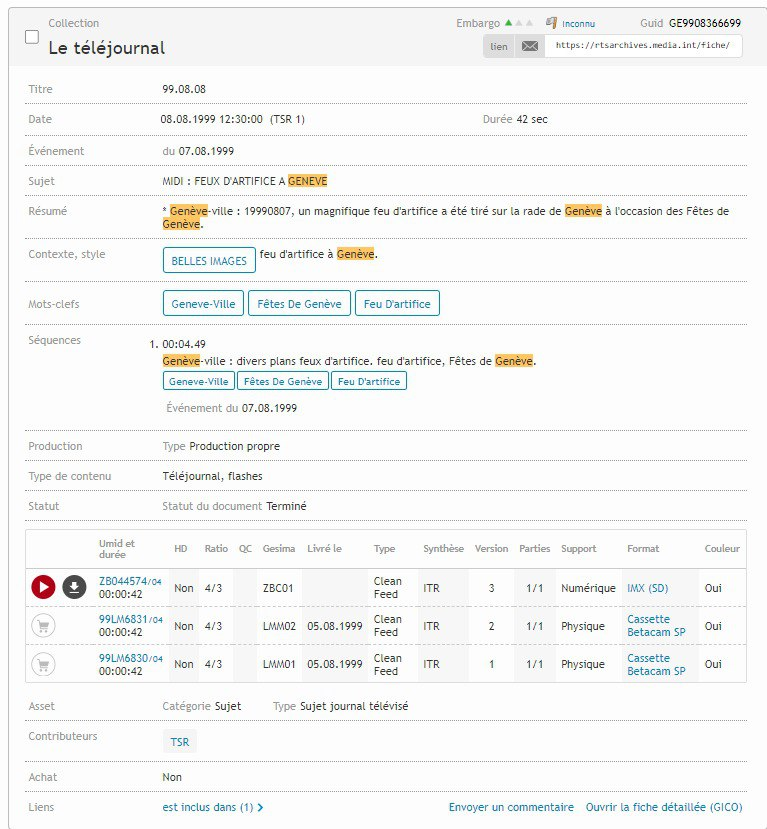
\includegraphics[width=0.8\textwidth]{images/image1.png}
	\caption{Exemple de fiche importée depuis l'outil GESIMA}
	\label{fig:image1}
\end{figure}


Le basculement vers GICO en 2014 a permis le moissonnage de métadonnées depuis divers canaux : d’abord la possibilité de faire le lien directement avec l’image numérique archivée en base grâce à l’ajout des time code ; puis en 2019 l’arrivée des données de production depuis l’outil Open Média (avec quelques problématiques d’encodage) et depuis Watson, la base de données de la programmation (notamment le sous-titrage) et enfin le lancement et la mise en production en 2022 d’outils d’Intelligence artificielle\index{Intelligence artificielle|see{IA\index{IA}}} : l’un de reconnaissance des locuteurs par leurs voix, l’autre de reconnaissance faciale des personnalités passant à l’antenne\footcite{sonderegger2024}, le dernier de \textit{speech-to-text}\footnote{C'est-à-dire qui retranscrit automatiquement les paroles en texte} (mis en production en 2019). Tous ces outils ont permis de réduire considérablement le temps de description effectué par les documentalistes, mais ont aussi le défaut de générer un bruit documentaire important.


\chapter{Se repérer dans un vaste ensemble : la repérabilité}

\subsection{Naviguer dans l'océan du web : l'importance du référencement}

« Le meilleur moyen de cacher un cadavre, c’est de le mettre en page 2 des résultats sur Google »\footnote{Il est très difficile de trouver un auteur à cette citation, très présente sur le web chez les professionnels du référencement\index{Référencement}. Elle a été lue sur \url{https://www.linkedin.com/pulse/le-meilleur-endroit-pour-cacher-un-cadavre-est-\%C3\%A0-la-page-loubier-/} sans pouvoir l’attribuer avec certitude à l’auteur de l’article.}, cette phrase, quoique assez provocante, illustre assez bien l’importance pour un contenu d’être placé en tête des résultats de recherche. Pour ce faire, les professionnels de ce qu’on appelle le référencement\index{Référencement} utilisent deux stratégies : le SEO (Search Engine Optimization), l'optimisation de la page pour qu’elle soit mieux affichée dans les résultats de recherche, et le SMO (Social Media Optimization), l'optimisation du contenu sur les réseaux sociaux pour qu’il génère plus de clics et soit plus vu (on parle de facteurs sociaux). C’est là le premier enjeu autour de la Repérabilité\index{Repérabilité} : pour qu’un contenu patrimonial ou un site soit repéré, il faut avant tout qu’il soit bien placé dans les résultats de recherche. Nous diviserons notre propos sur ce sujet en deux temps : d’abord « parler aux machines », où nous évoquerons les enjeux techniques spécifiques aux contenus patrimoniaux pour leur référencement\index{Référencement} ; puis « parler aux humains », où nous évoquerons les enjeux de communication et de valorisation. 

\subsection*{Parler aux machines}
« Rendre une information découvrable, dans un monde numérique, c’est la rendre accessible sous forme de données, la lier à d’autres informations pour que nos traces numériques se déploient, à l’image des réseaux de neurones dans le corps humain »\footnote{Josée Plamondon, \textit{Bien documenter pour favoriser la découverte en ligne : travailler avec les métadonnées}, rapp. tech., Canada, Fondation Jean-Pierre Perreault, 2019, \url{https://numerique.banq.qc.ca/patrimoine/details/52327/4020619}, pp. 13-14, cité dans \textit{Rapport - Mission franco-québécoise sur la découvrabilité en ligne des contenus culturels francophones}, Ministères de la Culture de la France et du Québec, France, Québec, Ministère de la Culture, 2020, p. 60, \url{https://www.culture.gouv.fr/Media/medias-creation-rapide-ne-pas-supprimer/Rapport-Mission-franco-quebecoise-sur-la-decouvrablilite-en-ligne-des-contenus-culturels-francophones.pdf}.}.

Cette citation éclaire très bien l’importance de ce que nous appelons un dialogue avec les machines, qui est le premier levier (en plus de celui de la Disponibilité\index{Disponibilité} des ressources en ligne déjà mentionné) vers la découvrabilité. Si une ressource n’est pas visible sur les moteurs de recherche, elle aura des chances moindres d’être découverte. Il nous faut donc évoquer les enjeux techniques du référencement\index{Référencement}, et pour cela, il nous faut d’abord comprendre le fonctionnement des moteurs de recherche. Nous nous focaliserons ici sur Google, car il concentre environ 90 \% de part de marché\footcite{zotero-245} et que son fonctionnement illustre celui de tous les autres moteurs de recherche. 

Ce qui a fait, dès sa création en 1998, la popularité de Google, c’est son algorithme (PageRank) qui a très sensiblement amélioré les résultats des recherches sur le web d’alors, où l’habitude était plutôt d’utiliser des annuaires tels que Yahoo, car les résultats des moteurs de recherche d’alors n’étaient que peu pertinents et très facilement falsifiables. Les créateurs de sites créaient par exemple, sous leur page web, une page blanche avec des milliers d’occurrences du terme auquel ils souhaitaient être associés pour être placés en tête des résultats\footcite[§ 4]{cardon2013}.


\begin{figure}[h!]
	\centering
	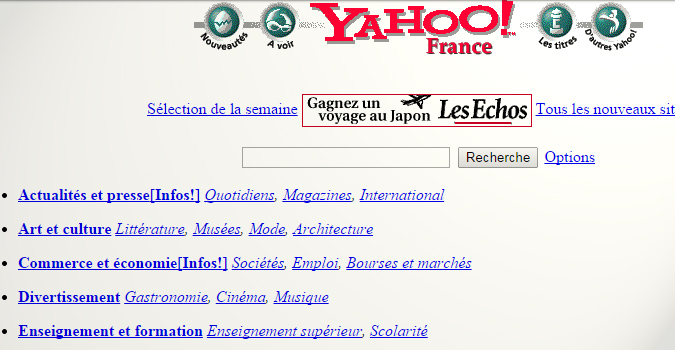
\includegraphics[width=0.4\textwidth]{images/image2.jpg}
	\caption{L'interface de Yahoo qui était au départ un annuaire }
	\label{fig:image2}
\end{figure}


L'efficacité de \textit{PageRank} est possible grâce à son utilisation d’une science inventée par Eugène Garfield : la scientométrie, au départ pour faciliter le travail des chercheurs et révéler les associations entre articles scientifiques, et les classer par nombre de citations\footcite[§ 5]{cardon2013}. Traduit dans le domaine du web, plus une page a de liens pointant vers elle (on utilise souvent le terme de backlinks), plus elle sera considérée comme centrale sur un sujet et donc pertinente. Ce principe fondamental de l’algorithme de Google a depuis été complété par un nombre impressionnant et toujours mouvant de critères, estimés à plusieurs centaines : mots-clés présents sur la page, confiance accordée au site, facteurs sociaux, temps de chargement\footcite{ertzscheid2019}… Google ne communique jamais sur ces critères afin d’éviter des pratiques d’optimisation abusives, leur conseil est toujours le même : « faites le nécessaire pour satisfaire au mieux les internautes qui visitent votre site web et ne vous préoccupez pas inutilement des algorithmes ou des paramètres utilisés par Google pour le classement »\footcite{zotero-236}. En plus de produire du contenu de qualité et utile pour les internautes, Google recommande aussi des pratiques techniques et notamment l’utilisation de « données structurées ». Pour illustrer leur importance, nous allons prendre l’exemple du projet data.bnf.fr de la Bibliothèque nationale de France (BnF).

\subsubsection{Data.bnf.fr : sortir les données du web profond}

Lancé en 2009, le projet data.bnf.fr a pour objectifs de favoriser la visibilité des données de la bibliothèque sur le web ; de casser les silos que constituent les multiples catalogues de l’institution en les regroupant en un point d’entrée unique ; de « faciliter la réutilisation des métadonnées par des tiers » ; de « contribuer à la coopération et l’échange de métadonnées par la création de liens entre des ressources structurées et de confiance »\footcite{s.d.}. En bref, de « rendre les données de la Bibliothèque nationale de France plus utiles sur le web ». Pour ce faire, data.bnf.fr utilise le modèle IFLA-LRM\index{Modèles de données!IFLA-LRM} (ex. FRBR\index{Modèles de données!FRBR}) qui est structuré comme suit (de façon synthétique) : l’œuvre d’un auteur est manifestée dans une édition matérialisée dans un item. Par exemple, \enquote{Notre-Dame de Paris} de Victor Hugo est manifesté dans une traduction anglaise qui est éditée chez \textit{Penguin Classics} et matérialisée dans un livre\footcite{bermes2023}.


\begin{figure}[h!]
	\centering
	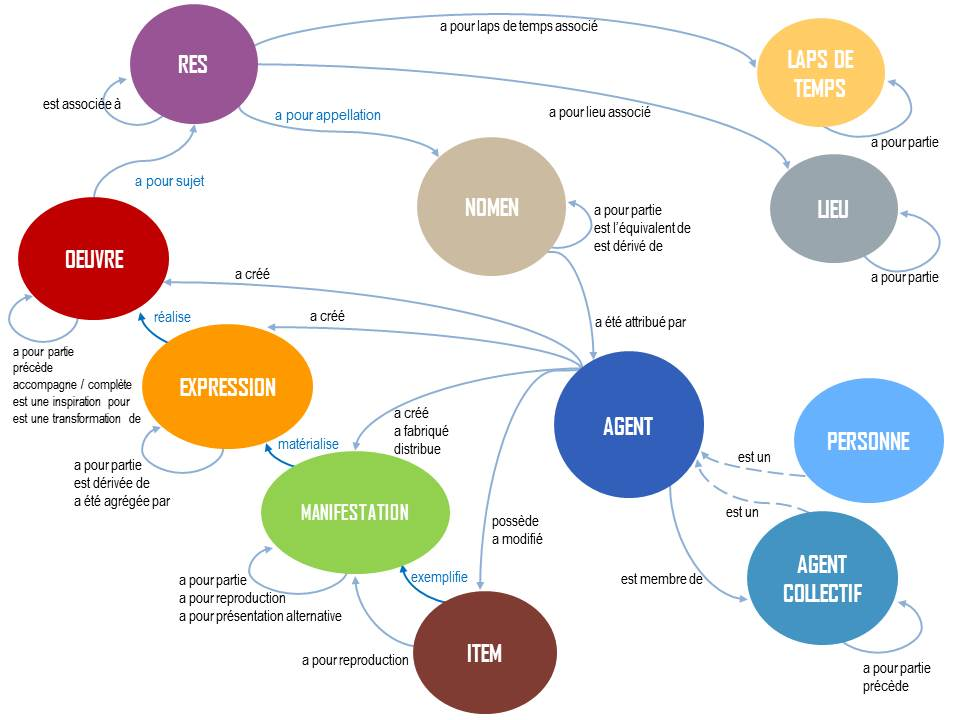
\includegraphics[width=0.8\textwidth]{images/image3.jpg}
	\caption{Illustration schématique du modèle FRBR/LRM}
	\label{fig:image3}
\end{figure}

\begin{center}
	Depuis : \url{https://data.bnf.fr/fr/semanticweb}
\end{center}



Le site (data.bnf.fr) va donc puiser dans les différentes sources de données de la BnF, qui sont dans différents formats de données : XML-EAD, Intermarc, etc. pour ensuite les structurer selon le modèle de graph-RDF (Resource Description Framework) qui est structuré en triplets : sujet, prédicat et objet. Cela donne en suivant notre exemple de tout à l’heure : Victor Hugo (sujet) a écrit (prédicat) \enquote{Les Misérables} (objet). L’avantage d’utiliser RDF est que l’usage des triplets facilite l’interconnexion et le partage, le modèle est souvent utilisé avec des ontologies, qui sont des descriptions formelles des concepts et des relations dans un domaine particulier, afin de standardiser et structurer les données. Cela améliore l’Interopérabilité\index{Interopérabilité} entre différentes bases de données et systèmes, et optimise le référencement\index{Référencement} des données sur le web, car cela rend plus claire leur structure pour un moteur de recherche\footcite{zotero-238}.

Par ailleurs, pour encore favoriser le référencement\index{Référencement}, data.bnf.fr utilise l’ontologie schema.org, créée justement par Google, Microsoft (Bing) et Yahoo (entre autres)\footcite{zotero-237} afin d’améliorer l’indexation des données (et son équivalent pour les réseaux sociaux, OpenGraph Protocol). De plus, data.bnf.fr expose ses données au format JSON-LD, qui permet encore d’améliorer l’indexation, mais aussi d’utiliser les fonctionnalités spéciales de recherche\footcite{zotero-236}.


\begin{figure}[h!]
	\centering
	\begin{minipage}[b]{0.45\textwidth}
		\centering
		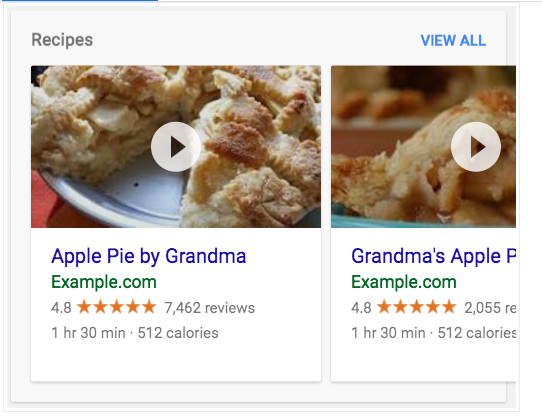
\includegraphics[width=\textwidth]{images/image4.png}
		\caption{Affichage pour l'utilisateur grâce aux données du \textit{knowledge graph}}
		\label{fig:image4}
	\end{minipage}
	\hspace{0.05\textwidth} % Espace entre les deux images
	\begin{minipage}[b]{0.45\textwidth}
		\centering
		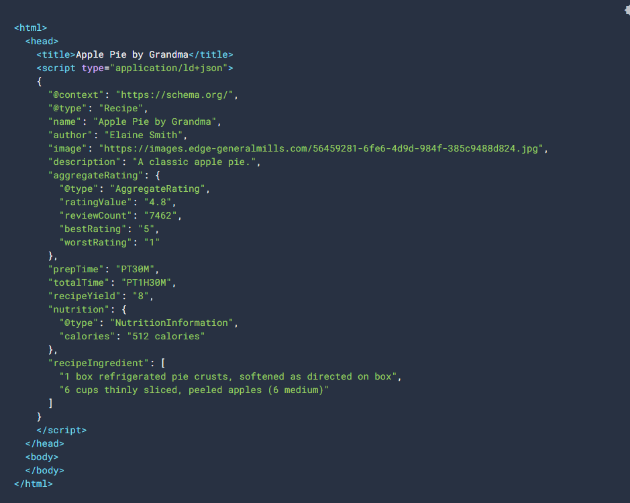
\includegraphics[width=\textwidth]{images/image5.png}
		\caption{Les données en question, affichage pour les machines}
		\label{fig:image5}
	\end{minipage}
\end{figure}
\begin{center}

Depuis :  \url{https://developers.google.com/search/docs/appearance/structured-data/intro-structured-data?hl=fr#search-appearance}

\end{center}
En plus de favoriser l’indexation des ressources, data.bnf.fr utilise des identifiants uniques pour chaque ressource (URI), pérennes (ce qui favorise aussi le référencement\index{Référencement}) qui permettent aux autres bases de données de pointer vers data.bnf.fr, et inversement. Par exemple, sur Wikidata, qui est structuré selon les mêmes principes que data.bnf.fr, la page Victor Hugo pointe vers la notice du Catalogue\index{Catalogue} général de la Bibliothèque grâce à son identifiant et cette dernière pointe vers l’identifiant Wikidata de l’auteur. Outre le fait que cela génère des \textit{backlinks}, cela permet aux moteurs de recherche de comprendre que le Victor Hugo de Wikidata est le même que celui de la Bibliothèque nationale et donc de lier entre-elles les données.

On l’a vu, en « parlant aux machines », data.bnf.fr a permis à ses ressources de sortir du web profond. Projet précurseur, il a été suivi par le Service interministériel des archives de France qui lançait en 2017 le portail\index{Portail} France archives, lequel met en œuvre les mêmes principes en ajoutant la fédération des fonds sur tout le territoire (ce que fait le Catalogue\index{Catalogue} collectif de France pour la Bibliothèque nationale de France). Force est de constater que les deux projets améliorent grandement le référencement\index{Référencement}. Si je tape par exemple la capitale du Dauphiné, c’est un extrait de Gallica qui m’est proposé par Google ; si je tape « archives Simone Veil », France Archives, le portail\index{Portail} français des archives\footnote{Nous reviendrons en détails sur la question des portails dans notre partie 2}, apparaît en deuxième position derrière une communication autour de l’exposition consacrée à Simone Veil par les archives nationales.

\begin{figure}[h!]
	\centering
	\begin{minipage}[b]{0.45\textwidth}
		\centering
		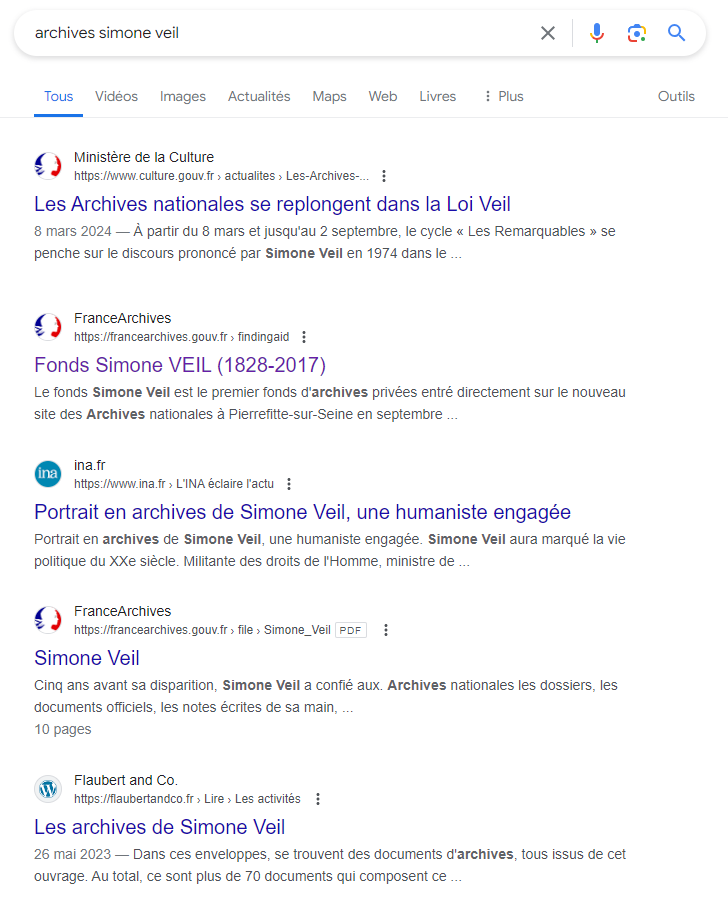
\includegraphics[width=\textwidth]{images/image6.png}
		\caption{\enquote{Archives Simone Veil}, résultats de recherche Google effectuée le 18 juillet 2024}
		\label{fig:image6}
	\end{minipage}
	\hspace{0.05\textwidth} % Espace entre les deux images
	\begin{minipage}[b]{0.45\textwidth}
		\centering
		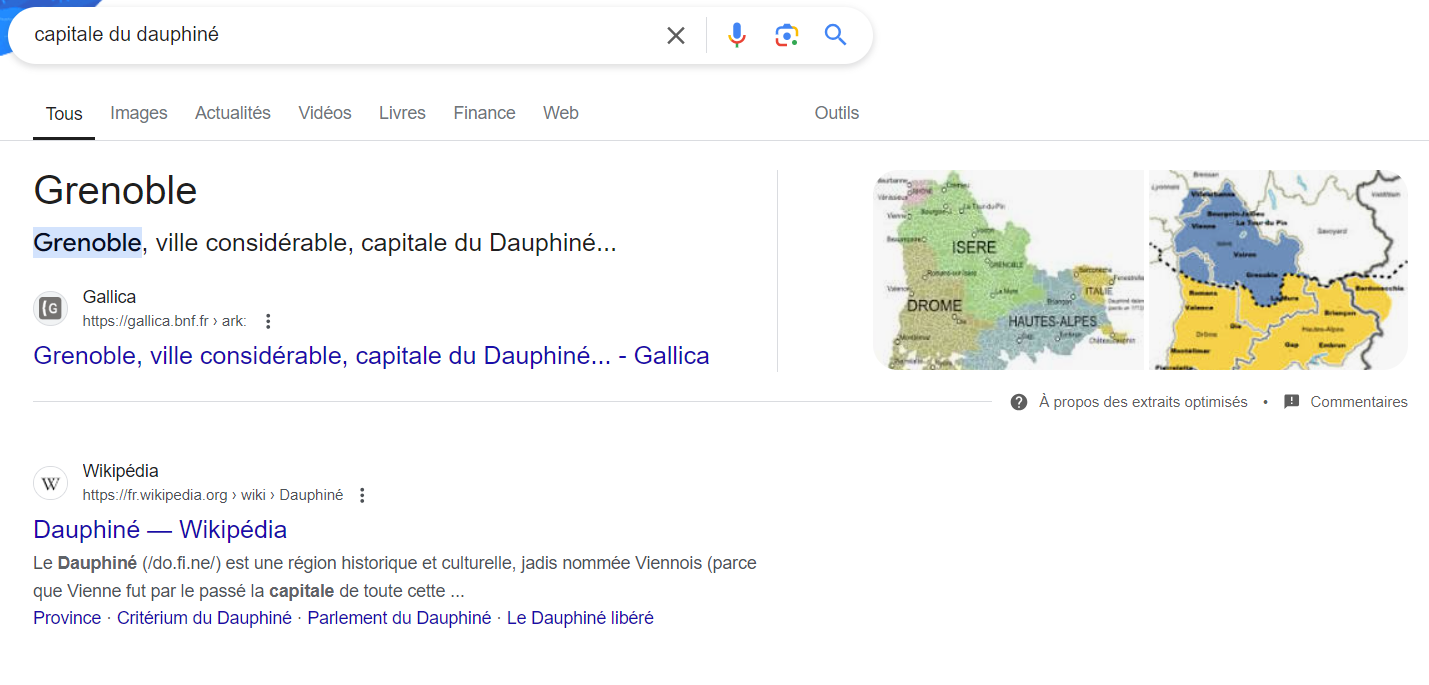
\includegraphics[width=\textwidth]{images/image7.png}
		\caption{\enquote{Capitale du Dauphiné}, résultats de recherche Google effectuée le 27 juillet 2024}
		\label{fig:image7}
	\end{minipage}
\end{figure}


En observant les résultats, on note deux choses : d’abord, Google génère automatiquement des réponses aux questions des utilisateurs (on parle alors de réponse zéro clic), parfois en se basant sur les données de la BnF, car les données du Knowledge graph\index{Knowledge graph} utilisées pour afficher ces questions utilisent les mêmes formats (JSON-LD)\footcite{zotero-235}, que ceux mis en œuvre par data.bnf.fr, mais surtout, les deux reposent sur les principes du web sémantique. D’où une « prime » accordée à ces données dans le référencement\index{Référencement} (en plus de tout ce qui a déjà été dit). Notons aussi que le premier résultat pour notre recherche sur Simone Veil est un contenu éditorialisé « pour les humains », car tout ce que nous venons de décrire est surtout utile pour que la machine comprenne bien le contenu des pages, mais est rarement consulté réellement ; en revanche, le contenu éditorial l’est plus et ce sera l’objet de notre prochaine partie où nous détaillerons l’importance de la valorisation patrimoniale dans une stratégie de référencement\index{Référencement} en prenant l’exemple de la RTS.

\subsection{Parler aux humains : l'exemple des archives de la RTS}

Si la stratégie technique de valorisation des contenus patrimoniaux est essentielle comme décrite plus haut, car elle permet aux machines de bien comprendre le contenu et les données, cette dernière n’aurait que bien peu d’intérêt si elle n’était pas accompagnée d’une stratégie de valorisation humaine : il est inutile de bien référencer une page dont le contenu est uniquement brut. Par ailleurs, les moteurs de recherches valorisent un contenu utile et de qualité et les réseaux sociaux sont bien souvent la porte d’entrée vers les sites web tout en améliorant leur référencement\index{Référencement}\footcite{laura2022}. Dans cette partie, nous nous concentrerons sur la stratégie de valorisation des archives de la RTS, car elle nous semble rassembler les grands enjeux du domaine : un fonds à l’immense volumétrie, des publics variés, et un environnement très concurrentiel.
\footnote{Josée Plamondon, Bien documenter pour favoriser la découverte en ligne : travailler avec les métadonnées, rapp. tech., Canada, Fondation Jean-Pierre Perreault, 2019, url : \url{https://numerique.
		banq.qc.ca/patrimoine/details/52327/4020619}, p. 14.cité dans : \textit{Rapport - Mission franco-québécoise sur la découvrabilité en ligne des contenus culturels francophones}, Ministères de la Culture de la France et du Québec, France, Québec, 2020, p. 60, \url{https://www.culture.gouv.fr/Media/medias-creation-rapide-ne-pas-supprimer/Rapport-Mission-franco-quebecoise-sur-la-decouvrablilite-en-ligne-des-contenus-culturels-francophones.pdf}}



\subsubsection{La \enquote{Bibliothèque de l'Honnête Homme} comme stratégie de valorisation }


Avec environ 1 million d’heures d’archives, dont les trois quarts sont audios, la RTS dispose d’un immense fonds. Cependant, ce n’est pas sans poser de problèmes, comme évoqués dans notre première partie : l’impossibilité d’appréhender dans leur totalité des objets culturels complexes générant une Fatigue muséale\index{Fatigue muséale} qu’il est difficile de contrer « much like death and taxes »\footnote{Bitgood, 2009, cité dans Windhager (Florian), Salisu (Saminu), Schreder (Günther) et Mayr (Eva), « Orchestrating Overviews : A
	Synoptic Approach to the Visualization of Cultural Collections », Open Library of Huma-
	nities, 4–2 (août 2018), \url{doi : 10.16995/olh.276.}}. Même si elle en aurait la possibilité\footnote{Hors quelques archives dont les droits ne lui appartiennent pas.}, la RTS fait le choix de ne pas donner à voir toute sa collection : ni sur le site dédié, ni sur les réseaux sociaux qu’elle anime, consciente du fait que montrer la masse documentaire presque infinie noierait les documents intéressants. La stratégie est donc celle d’une éditorialisation et d’une contextualisation riche, le défi est donc, comme le notent F. Windhager et al. (trad.) « de rendre les collections compréhensibles malgré une vision limitée et à des capacités d’attention restreintes »\footcite[p. 3]{windhager2018a}.

Ainsi, le site\footnote{\url{ https://www.rts.ch/archives/}} est organisé comme une « Bibliothèque de l’Honnête Homme »\footcite{chatelain2003} : suivant quelques thématiques, avec à chaque fois un nombre relativement restreint d’archives toujours éditorialisées, parfois assez sommairement, parfois de façon détaillée suivant une écriture journalistique\footnote{\url{ https://www.rts.ch/archives/grands-formats/9614551-on-a-tue-bob-kennedy.html}}, ce qui favorise le référencement\index{Référencement}. Par ailleurs, les rebonds entre différents documents sont favorisés de deux manières : leur classement dans des dossiers thématiques et les recommandations, manuelles, faites par les documentalistes (nous reviendrons en détail sur la notion de Recommandation\index{Recommandation}).


\begin{figure}[h!]
	\centering
	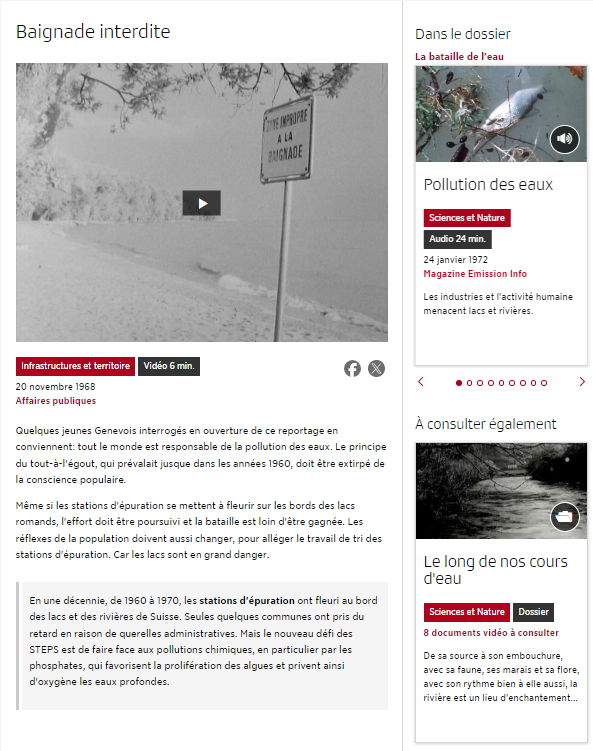
\includegraphics[width=0.8\textwidth]{images/image8.png}
	\caption{\enquote{Baignade interdite}, exemple de recommandation proposée par les documentalistes de la RTS}
	\label{fig:image8}
\end{figure}


\subsubsection{L'importance du SMO (social media optimisation)}


En 2024, sur les 5,35 milliards d’utilisateurs que compte le web, 5,04 milliards disposent d’un compte sur un réseau social\footcite{zotero-229}. Il est évident qu’il est impossible de les ignorer dans une stratégie de Repérabilité\index{Repérabilité} et de référencement\index{Référencement}. C’est doublement vrai, car, d’abord — comme évoqué plus haut — une présence efficace sur les réseaux sociaux améliore le référencement\index{Référencement} dans les moteurs de recherche, on parle de SMO (social media optimisation) ; ensuite, être visible sur ces derniers génère un nombre non négligeable de clics vers les contenus, car ils représentent un tiers du temps passé en ligne\footcite{zotero-227}.

Dans le cas des archives de la RTS, ce sont clairement les réseaux sociaux qui sont le principal canal de diffusion des archives et de réception. L’institution est présente sur Facebook (490 000 followers), Instagram (115 000 followers), YouTube (607 000 abonnés), suivant la fameuse phrase de Marshall McLuhan « The medium is the message »\footcite{zotero-226} : chaque plateforme a un contenu unique et adapté. Ainsi, Instagram est alimenté en contenus courts, YouTube est le canal des formats longs, et Facebook des formats de moyenne durée. Par ailleurs, les archives sont publiées au format horizontal (plus adapté pour une consultation sur ordinateur) sur toutes les plateformes sauf Instagram, qui cible clairement un public plus jeune, sur son smartphone.


\chapter{Émerger dans le lac d'une collection : la Recommandation}

\subsection{Sérendipité\index{Sérendipité} : quand l'heureux hasard rencontre les algorithmes}

« On ne trouve sans chercher que quand on a beaucoup cherché sans jamais trouver »\footcite{2015}, cette citation illustre bien le concept de Sérendipité\index{Sérendipité} qui se définit comme le « don de faire par hasard des découvertes fructueuses »\footcite{zotero-224} et qui est tiré de l’anglais \textit{serendipity}, néologisme créé en 1754 par Horace Walpole à partir du conte oriental « les trois principes de Serendip », Serendip étant ici le nom ancien du Sri Lanka composé des deux mots sanscrits \textit{Sri} « souveraineté, richesse, éclat » et \textit{Lanka}, rapproché du grec \textit{lagkanein} « obtenir par le sort »\footcite{zotero-224}. La Sérendipité\index{Sérendipité} serait donc, étymologiquement, l’obtention de richesses grâce au sort, mais cette définition semble réductrice par rapport à l’usage qui a été fait de ce mot. Il est en effet utilisé pour désigner des découvertes fortuites certes, mais qui ne sont jamais le total fruit du hasard. Si Flemming a découvert, par Sérendipité\index{Sérendipité} (il aurait oublié des cultures de moisissures à son départ en congé), la pénicilline : c’est qu’il la cherchait ; de même, Archimède s’écriant « Euréka » dans sa baignoire alors qu’il cherchait un moyen de prouver que la couronne d’Hiéron II était composée d’or entièrement\footcite[Annexe 1]{michel2019}. Ces deux exemples illustrent le fait que la Sérendipité\index{Sérendipité} est autant le fruit du hasard que de la « recherche sans jamais trouver » : c’est parce que Flemming et Archimède avaient dans leur saillance perspective\footnote{Concept sémiologique qui s’illustre bien par l’exemple suivant : à l’achat d’un vélo, on devient tout de suite très sensible à toutes les potentialités pour l’accrocher (grilles, poubelles, plots dans la rue, etc.). in Marc Jahjah, introduction à la sémiologie, cours de 1ère année de DUT information et communication, 2018 } la recherche d’une solution à leur problème.

Si au même moment, et pour les mêmes raisons que le terme de découvrabilité, le terme de Sérendipité\index{Sérendipité} réémergeait en 2011, selon Francis Balle, c’est bien que les deux termes sont liés : la découvrabilité comme la Sérendipité\index{Sérendipité} ne sont pas inhérentes au web, les usagers des bibliothèques le savent bien, mais tout comme la découvrabilité, en mettant au jour d’incroyables perspectives de Sérendipité\index{Sérendipité} (la masse non classée permet de voir des choses inattendues), le web et ses Données massives\index{Données massives} semblent aussi poser le problème. D’une navigation riche en découvertes, on peut vite se « perdre dans l’hyperespace »\footnote{Selon le livre éponyme de Quentin Quick et J. Schaherpenhuizen} et de la Sérendipité\index{Sérendipité}, on passe alors à la zemblanité : où toutes les découvertes ne viennent qu’enfoncer des portes ouvertes\footcite[§ 10]{michel2019}. Il faut ici distinguer trois types de navigation sur internet : la première est celle où l’utilisateur souhaite trouver une information précise sur un sujet, il va alors saisir une équation dans un moteur de recherche, par exemple « Sérendipité\index{Sérendipité} » ET « Web » (Sérendipité\index{Sérendipité} quasi nulle)\footcite[p. 8]{ertzscheid2003} ; la deuxième est une navigation à proprement parler en utilisant les liens hypertextes d’une page ou d’un article (Sérendipité\index{Sérendipité} structurelle)\footcite[p. 8]{ertzscheid2003} ; la troisième est basée sur l’apprentissage, l’utilisateur sait qu’il ne sait pas ce qu’il cherche (Sérendipité\index{Sérendipité} associative)\footcite[p. 8]{ertzscheid2003}. Ces liens hypertextes sont l’une des spécificités d’internet, inventés en 1960 par Ted Nelson, sur base des travaux menés dès 1945 de Vannevar Bush et son Memex (il écrit dans son article « \textit{As we may think} » que le cerveau humain fonctionne par association d’idées et non de façon linéaire)\footcite{vanevarbush1945}, ils viennent casser la linéarité de lecture traditionnelle d’un texte en ajoutant des liens sémantiques activables par le lecteur\footcite{14}. Cette rupture de linéarité est un élément fondamental de la Sérendipité\index{Sérendipité} sur le web, selon Olivier Ertzscheid et Gabriel Gallezot les liens hypertextes permettent « la mise en relation des unités informationnelles [...] [cela] peut permettre de découvrir des corrélations insoupçonnées »\footcite{zotero-221}. Insoupçonnées est ici un mot important, il ne s’agit jamais de hasard : ce dernier n’existe pas sur le web, les algorithmes, défini comme « suite finie et non ambigüe d’instructions et d’opérations permettant de résoudre une classe de problèmes »\footcite{2024a} rendent totalement impossible la création de hasard puisque chacune de leurs actions sont déterminées à l’avance, et même s’ils peuvent donner l’illusion de hasard (par la masse de données traitées notamment), ce dernier n’est jamais complet. Par ailleurs, il faut noter que les logiques marchandes du web, organisé en un « capitalisme linguistique »\footnote{Ce concept sera traité dans la partie 3, il est issu de l'article de Frédéric Kaplan paru dans le Monde Diplomatique en 2011 : \url{https://www.monde-diplomatique.fr/2011/11/KAPLAN/46925 }} et autour du concept d’Économie de l’attention\index{Économie de l’attention} semblent s’opposer à toute Sérendipité\index{Sérendipité}.

Afin d’illustrer notre propos, prenons deux exemples, l’un tiré d’un site à but non lucratif : Wikipédia et l’autre tiré d’un site à la logique marchande, Mix.com (ancien StumbleUpon). Le premier, qu’on ne présente plus, en plus de disposer d’une fonctionnalité « article aléatoire » est structuré de manière à favoriser la navigation entre les articles. Par exemple, en commençant notre lecture sur l’article « Sérendipité\index{Sérendipité} », nous avons eu connaissance d’un article écrit par Olivier Ertzscheid et Gabrielle Gallezot sur ce sujet en lien avec la recherche d’information. Connaissant préalablement bien les travaux d’Olivier Ertzscheid, nous avons décidé de consulter cet article qui s’est révélé déterminant. Wikipédia favorise donc la Sérendipité\index{Sérendipité} par la présence nombreuse de liens hypertextes d’une part (Sérendipité\index{Sérendipité} structurelle), mais aussi, de l’autre : par la présence des sources en bas de chaque article, souvent point de départ de fructueuses recherches. Il nous faut en revanche présenter le site Mix.com (ex-StumbleUpon), ce dernier est basé sur un principe simple : proposer à ces utilisateurs des images/vidéos aléatoires selon leurs centres d’intérêt. Ainsi, à l’inscription sur le site, il est demandé à chaque utilisateur d’en choisir quelques-uns parmi des catégories précréées, le site lui propose ensuite une quasi-infinité d’images moissonnées depuis d’autres médias sociaux tels que Redit ou X (ex-Twitter) qu’il peut, ou non « aimer » pour que l’algorithme lui propose plus d’images du même type. Le site lui propose, dans le même temps, des images liées à ce qu’il voit.


\begin{figure}[h!]
	\centering
	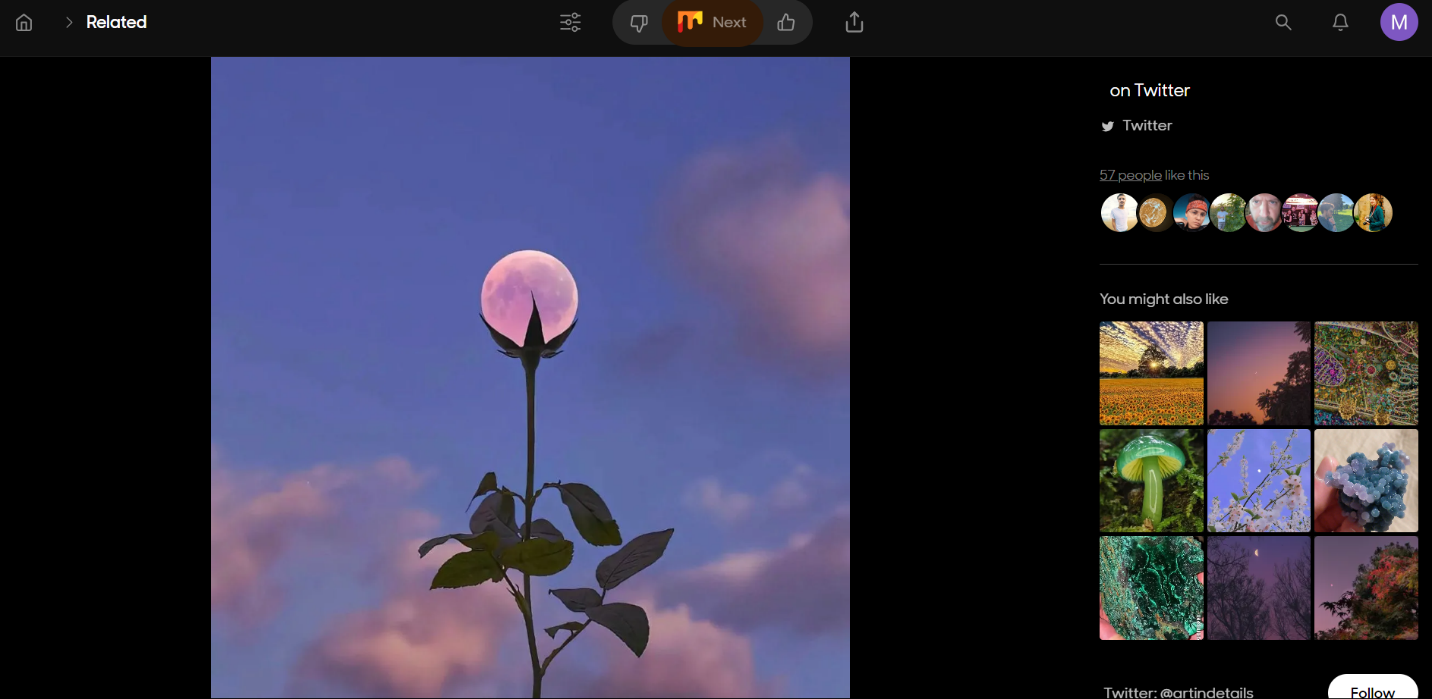
\includegraphics[width=0.8\textwidth]{images/image9.png}
	\caption{L'interface de Mix.com}
	\label{fig:image9}
\end{figure}


On a donc une Sérendipité\index{Sérendipité} qui semble associative : l’utilisateur ne sait pas ce qu’il cherche, mais, à force de naviguer et d’affiner ses gouts, il finira par « tomber » sur quelque chose d’intéressant. Sauf qu’ici, le modèle économique, anciennement nommé \textit{StumbleUpon paid discovery} propose à des annonceurs de payer pour voir leur contenu propulsé à des utilisateurs, cassant ainsi le principe de Sérendipité\index{Sérendipité} au profit d’une logique marchande très puissante puisque l’utilisateur croira que la publicité lui est destinée personnellement et sera bien plus enclin à la consulter : c’est tout l’intérêt des algorithmes de Recommandation\index{Recommandation}\footcite{author2012}.

Finalement, de même qu’une bibliothèque par son organisation physique suivant des classifications arbitraires (citons Dewey par exemple) créé en quelque sorte une « Sérendipité\index{Sérendipité} artificielle » où les lecteurs en déambulant peuvent faire de belles découvertes, mais uniquement s’ils s’ouvrent au hasard, la Sérendipité\index{Sérendipité} comme décrite par Eva Sandri va « au-delà de l’heureux hasard, il s’agirait donc d’un état de Disponibilité\index{Disponibilité}, de réflexivité et d’ouverture d’esprit qui ferait en sorte de considérer l’erreur comme constructive »\footcite[p. 14]{zotero-221}. Il semble qu’on puisse conclure de la même chose pour le web : si un utilisateur s’ouvre aux heureux hasards que peut lui proposer une navigation hypertextuelle, il pourra « tomber » sur des choses intéressantes. L’immense avantage du web est qu’il n’est justement pas organisé en grandes classifications arbitraires, la navigation est donc ici interdisciplinaire « car l’internet n’a pas de frontières »\footcite[8 minutes 34 secondes]{2015} ; son immense inconvénient est en revanche les risques pour l’utilisateur de se perdre totalement dans la masse des propositions de navigation qu’il reçoit sans cesse. Les algorithmes de Recommandation\index{Recommandation} peuvent alors être vus comme la solution à ce problème de la masse : en ciblant leurs utilisateurs de façon très précise et en leur proposant du contenu proche de celui qu’ils viennent de consulter, ce sont à la fois des outils de création de Sérendipité\index{Sérendipité}, mais aussi des outils d’enfermement algorithmique régis parfois par des logiques marchandes (cf. exemple de Mix.com). Ils seront l’objet de notre prochaine partie.


\subsection{Les algorithmes de Recommandation}



Avant toute chose, il nous faut tâcher d’expliquer le fonctionnement technique des algorithmes de Recommandation\index{Recommandation}. Ces derniers ont pour objectif de rapprocher, selon des critères définis (genre, type d'utilisateur ayant regardé...), deux objets (films, musiques, textes…). Pour tâcher d’être le plus clair possible, prenons un cas d’usage : admettons que l'on souhaite rapprocher tous les programmes ayant la même thématique dans le fonds de la RTS ; nous avons pour cela à notre disposition trois choses : une transcription, un résumé et des mots-clés définis à partir d’un thésaurus. Par différentes opérations mathématiques, on va transformer ces trois éléments en un chiffre entre 0 et 1\footnote{  Dans notre cas, on utiliserait un algorithme de type TF-IDF qui calcule la fréquence (Term Frequency [TF]) d’un terme dans un document en calculant le nombre de fois où le mot apparait divisé par le nombre de mots totaux et sa rareté dans tous les documents (Inverse document Frequency [IDF]) en calculant le logarithme du nombre total de documents divisé par le nombre de documents contenant le mot, on fait ensuite TF * IDF. L’intérêt est d’identifier les mots signifiants importants pour un document en réduisant l’importance des mots vides (« le », « et »…) [Explications fournies par Chat-GPT et remaniées}. Ensuite, on place ce chiffre dans un espace vectoriel, c’est-à-dire dans un espace mathématique (voir image ci-après), le tout pour chaque archive. Les points qui sont proches sont ceux partageant des caractéristiques communes, puisque le chiffre qui a été calculé à partir de leurs métadonnées spécifiques est proche. Si l'on souhaite voir les documents (où les personnes en suivant leurs traces en ligne ou données démographiques) similaires, je n’ai qu’à prendre tous les points proches dans mon graphique\footcite{zotero-216}.


\begin{figure}[h!]
	\centering
	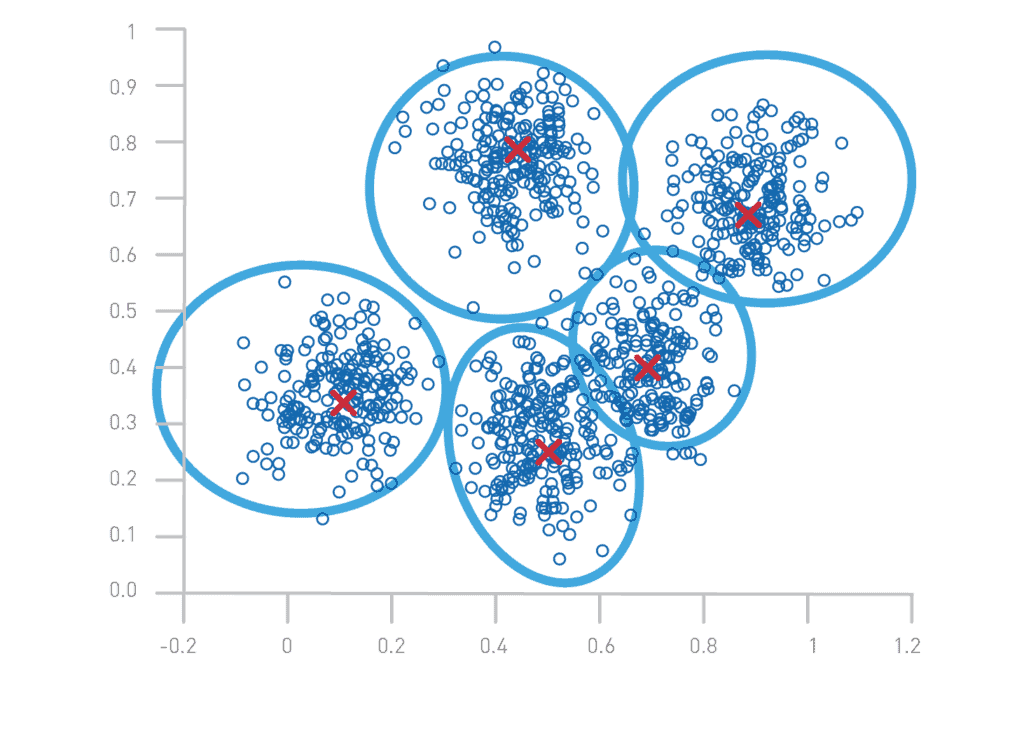
\includegraphics[width=0.8\textwidth]{images/image10.png}
	\caption{Fonctionnement schématique d'un algorithme de clustering}
	\label{fig:image10}
\end{figure}

\begin{center}
	\url{https://www.data-transitionnumerique.com/k-means/}   
\end{center}

Cette description est évidemment très simplifiée : comment délimiter les catégories entre elles ? Comment faire en sorte que mon algorithme classe tous les documents selon des thématiques définies et pas uniquement en prenant en compte, par exemple, leur champ lexical ? Mais le principe des algorithmes de Recommandation\index{Recommandation} est grossièrement celui décrit. Il a été expérimenté dès 1975 par Salton et al.(cité par Arnaud Claes)\footcite[p. 38]{claes2022}. En 2002, Robin Burke proposait de répartir les algorithmes de Recommandation\index{Recommandation} selon cinq catégories\footcite{claes2022} :

\begin{itemize}
	\item Recommandation\index{Recommandation} collaborative : Les contenus sont proposés en fonction des préférences de l’utilisateur et des comportements d’autres utilisateurs similaires.
	\item Recommandation\index{Recommandation} basée sur le contenu : Les suggestions sont faites en fonction des éléments similaires consultés par l’utilisateur dans le passé.
	\item Recommandation\index{Recommandation} démographique : Les recommandations sont établies sur la base de critères démographiques tels que l’âge, le sexe et la localisation.
	\item Recommandation\index{Recommandation} basée sur un modèle de connaissance : Ces algorithmes utilisent une base de connaissances, construite grâce aux réponses de l’utilisateur à des questions spécifiques, pour suggérer des objets en fonction des besoins exprimés.
	\item Recommandation\index{Recommandation} basée sur l’utilité : Les contenus sont proposés en fonction de leur utilité pour l’utilisateur. Par exemple, si un arbre de décision pour le choix d’un produit prend en compte le coût, l’impact carbone et les notes des autres utilisateurs, un produit répondant à ces trois critères sera recommandé.
\end{itemize}

Sans rentrer dans le détail, chacune de ces catégories a des avantages et inconvénients : par exemple faire des recommandations basées sur le contenu nécessite beaucoup de données d’entraînement et de capter les traces de l’utilisateur, les recommandations basées sur l’utilité sont statiques, etc. C’est pourquoi elles sont souvent combinées, c’est par exemple le cas de Netflix qui utilise huit algorithmes différents, chacun répondant à un cas d’usage spécifique\footcite[p. 47]{claes2022}. Ce dont ces catégories témoignent, c’est aussi de deux visions : la première suppose que l’utilisateur peut explicitement donner ses préférences et la seconde, dite béhavioriste, suppose qu’il faut observer ses actions pour lui proposer du contenu\footcite[p. 38]{claes2022}. On observe clairement que la seconde vision décrite est celle qui est la plus représentée aujourd’hui, et ce, car les créateurs des algorithmes ont compris que « l’utilisateur n’est pas toujours la source la plus fiable pour éclairer ses propres intentions »\footcite[p. 39]{claes2022}. Force est de constater l’incroyable puissance de ces algorithmes quand on parle de découvrabilité, ainsi, si l’on prend l’exemple de Spotify et ses 80 millions de titres au Catalogue\index{Catalogue}, on peut noter que les playlists générées par algorithme de Recommandation\index{Recommandation} « découvertes de la semaine » jouent bien leur rôle. Elles auraient, en effet, permis — quelques mois après leur lancement — à quarante millions de personnes de consulter 5 milliards de morceaux nouveaux\footcite[§ 2]{durand_chapitre_2016-1}. Mais si le potentiel est immense, les enjeux le sont aussi, et notamment la transparence : comment savoir pour quelle raison tel contenu m’a été recommandé ? Surtout quand on voit à quel point les recommandations sont parfois grossières et fruits de clichés tenaces. Ainsi, en 2016, April Joyner, journaliste afro-américaine spécialisée dans les nouvelles technologies, se plaignait d’avoir vu, de façon soudaine un tiers de ses recommandations incluant des femmes afro-américaines dans les rôles-titres et l’apparition d’une catégorie « \textit{African American Movies} » sur sa page d’accueil. Elle y voit un écueil majeur : l’invisibilisation, si l’utilisateur ne cherche pas à regarder un film de ce type et n’est pas catégorisé comme probablement de cette ethnie (April Joyner vit à Harlem\footcite{2017}), il n’en verra jamais\footnote{La question des bulles de filtre sera traitée dans la partie 3}.

On a donc des algorithmes qui, clairement, offrent un potentiel énorme de découvrabilité, mais qui, s’ils sont utilisés à des fins commerciales, finissent par réduire le champ de la découverte. Pour que les institutions patrimoniales, et plus largement les acteurs publics, puissent s’emparer du potentiel de ces algorithmes tout en évitant les problèmes posés, on a depuis quelques années vu émerger la notion d’Algorithme de service public\index{Algorithme de service public} dont nous tâcherons d’observer les différences fondamentales avec ceux mis en œuvre par les acteurs privés.



\subsubsection{La notion d'Algorithme de service public : \enquote{prenez les commandes}, l'algorithme de Recommandation de Radio France}

Même si la société nationale de radiodiffusion française n’est pas un acteur patrimonial, l’ambition de son algorithme de Recommandation\index{Recommandation} est comparable à ceux évoqués par Irène Bastard et Arnaud Laborderie dans un article de juin 2023 réfléchissant à la mise en place d’un tel dispositif sur Gallica, la bibliothèque numérique de la Bibliothèque nationale de France\footcite{bastard2023}. C’est-à-dire : augmenter le taux de la collection qui est consultée par les individus (48 \% sur Gallica)\footcite{bastard2023} ; améliorer les rebonds entre les items (seuls 1 à 3 documents consultés par session en moyenne sur Gallica)\footcite{bastard2023} dans des collections où il est difficile de se repérer tout en évitant les écueils des algorithmes de Recommandation\index{Recommandation} commerciaux : Bulle de filtre\index{Bulle de filtre}, effets de viralité (quelques contenus reçoivent tous les clics), manque de transparence, perte de contrôle\footcite{2023b}.

Ces ambitions et craintes, pensées avec les équipes éditoriales de Radio France, ont ensuite été transformées en cinq grands principes : 
\begin{itemize}
	\item Mettre l’humain au cœur de la démarche de Recommandation\index{Recommandation} ;
	\item Être totalement transparent ;
	\item Favoriser la découverte et la curiosité tout en restant efficace ;
	\item Laisser le contrôle à l’auditeur\footcite{2023b}.
\end{itemize}

La différence fondamentale avec les algorithmes de Recommandation\index{Recommandation} privés est ici l’humain : il est au cœur de la démarche de Recommandation\index{Recommandation} (et même de conception de cet algorithme) ; il peut comprendre pourquoi tel contenu lui a été proposé et il peut refuser qu’on l’oriente algorithmiquement et orienter l’algorithme (en lui indiquant par exemple de favoriser une émission en particulier) : le tout, pour favoriser sa découverte, car aucun humain ne pourrait naviguer dans les deux millions d’heures du Catalogue\index{Catalogue} de Radio France pour recommander à chacun le programme qu’il est susceptible d’apprécier. La notion d’Algorithme de service public\index{Algorithme de service public} n’est donc pas tant technique ; certes les données d’usage (traces ou logs) collectées sont réduites ; certes aussi les algorithmes publics n’utilisent pas ou peu de données démographiques, mais ce qui est fondamentalement différent c’est qu’ils placent l’humain au cœur de leur démarche, il garde le contrôle sur ce qu’il voit, comprend pourquoi il le voit et peut décider de stopper à tout moment : il reste donc le « pilote » de sa navigation\footcite{ertzscheid2024a}, ce qui constitue, si l’on suit l’analyse d’Olivier Ertzscheid, un retour en arrière : 
« Longtemps les technologies nous ont placées en situation de pilotage, avant de nous reléguer au rang de copilote, puis en nous laissant copilote, mais en supprimant le pilote au profit d’une seule fonction de pilotage automatique, et nous voilà désormais simplement, inexorablement, irrévocablement… passagers. Passagers par ailleurs exposés à la permanence d’un contrôle identitaire, et passagers sans autre bagage que l’acceptation naïve d’imaginer que nous pourrions encore être maitres du choix de notre destination. »\footcite{ertzscheid2024a}

Et c’est peut-être parce que Radio France est déjà un acteur majeur de la découvrabilité culturelle au travers de ses antennes que la notion d’algorithme au service du public, où l’humain est au cœur de la démarche y a été si bien comprise. Pensons par exemple à FIP (France Inter Paris), radio de l’éclectisme musical diffusant plus de 40 000 titres différents par an\footcite{2023a}, et dont le directeur écrivait en 2023 qu’il possédait le meilleur algorithme du monde : « Pourquoi ? Tout simplement, car il est humain. Chaque jour, nos programmateurs partent d’une page blanche et programment — manuellement — des tranches de vie musicale dans lesquelles toutes les musiques se doivent de se mélanger »\footcite{2023a}.


 % Import de la partie 1
	


	%Document vide aux normes de l'École nationale des Chartes
%Dernières modifications E. Rouquette (12/2023)



\part{Partie 2 : Nouveaux catalogues, nouvelles interfaces, nouveaux usages}



%\setcounter{chapter}{0} % remet le compteur des chapitre à 1 

\chapter{Les interfaces : nouvelles architectures ?}
\begin{quote}
	\textit{2100, France, la Bibliothèque nationale vient d’achever la numérisation de l’entièreté de sa collection. Le site François-Mitterrand, reflet de « l’utopie numérique »\footcite[p. 20]{bermes2024} de son fondateur à savoir numériser et rendre accessibles tous les savoirs conservés et qui devait être l’objet d’une réfection globale ne sera finalement pas restauré, mais transformé en habitations, jugé inutile. Le conservatoire d’Amiens suffisant à conserver l’entièreté du dépôt légal entrant, devenu entièrement dématérialisé. La consultation, seule vocation du site François-Mitterrand, ayant été déplacée en ligne, ce dernier n'a plus d'intérêt. La bibliothèque, en tant qu’emprise physique et Lieu de mémoire\footnote{En référence aux ouvrages parus sous la direction de Pierre Nora entre 1984 et 1992} n’est plus : remplacée par l’interface\index{Interface} en ligne qui prend sa fonction symbolique, devant dès lors une architecture de pouvoir au sens propre ; volonté de la prestigieuse institution d’être le reflet de son histoire, nouveau Lieu de mémoire, elle concentre toutes les attentions.}
\end{quote}

Si évidemment cette uchronie est totalement fantasmée (cauchemardée ?) : il est inimaginable de voir les bibliothèques de consultation disparaître, elles qui mènent justement et avec brio des politiques centrées autour de l’accueil depuis des années. Il est tout aussi inimaginable de penser que le site François-Mitterrand pourrait devenir inutile face à une société totalement digitalisée : le relatif échec des livres numériques en est la preuve. Il est de toute manière impensable que la numérisation de la totalité des collections de la Bibliothèque nationale de France soit un jour une réalité, cela n’aurait pas d’intérêt et serait coûteux (et encore, par rapport aux archives nationales, la Bibliothèque nationale de France numérise beaucoup). Mais il nous semblait intéressant de pousser à l’extrême un mouvement qui est bien réel : les interfaces prennent peu à peu, mais sans jamais les remplacer totalement, le rôle des lieux de consultation et deviennent, de fait, des \textit{Lieux de mémoire numériques }en tant que premier accès pour une immense partie des citoyens à la connaissance conservée. Elles se définissent comme la « jonction entre deux matériels ou logiciels leur permettant d’échanger des informations par l’adoption de règles communes physiques ou logiques »\footcite{zotero-205} c’est-à-dire qu’elles assurent la médiation de l’accès au savoir, dans le cas des institutions patrimoniales ; l’interface\index{Interface} la plus courante est le catalogue\index{Catalogue}. Cette question des interfaces prend donc une place centrale dans la découvrabilité des collections par leur rôle de médiation, et après avoir parcouru les enjeux autour de la notion de découvrabilité, il est intéressant de s’attarder sur ces dernières et d’analyser leur importance et leurs mutations récentes.

\chapter{« Vers de nouveaux catalogues »}

\vspace{-3em} % Réduit l'espacement vertical pour que la référence soit proche du titre.

\textit{En référence au titre d’un ouvrage paru en 2016 sous la direction d’Emmanuelle Bermès.}

\subsection{La transition bibliographique}

Pour parler de nouveaux catalogues et tenter de montrer comment et par quels moyens ils améliorent la découvrabilité des collections patrimoniales, il nous semble important de commencer par le début en abordant les raisons ainsi que l’historique de ces mutations. Cela nous permettra de tenter de distinguer les pratiques réellement nouvelles et novatrices des autres. Pour cela, nous commencerons par aborder la transition bibliographique que David Aymonin, directeur de l’Agence bibliographique de l’enseignement supérieur (Abes) présente ainsi : « On peut présenter la transition bibliographique simplement en expliquant que c’est une façon d’exprimer les métadonnées décrivant les documents sous forme d’entités et de relations. Cela fait presque 15 ans [en 2022, N.D.A] maintenant que les communautés de professionnels y travaillent, dans un monde de la documentation où tout est en transition. Nous avons le projet de partager les données de nos catalogues pour créer de nouveaux services […] il s’agit de créer des données riches, liées et accessibles à tous et sur lesquelles chacun peut s’appuyer pour les enrichir et développer de nouveaux services, de nouvelles activités, de nouvelles industries »\footcite[§3 et §4]{carre-marillonnet_transition_2022}. Ce programme a été mis en place conjointement par l’Abes et la Bibliothèque nationale de France et suit une logique mondiale impulsée par l’OCLC (la coopérative mondiale des bibliothèques).

Il s’appuie sur les principes de Paris, qui sont le cadre normatif du catalogage depuis 1961 avec en ligne de mire l’harmonisation des pratiques à l’échelle mondiale pour faciliter les échanges de notices et qui marquent la fin des catalogues sous forme de volumes papier et leur apparition sous forme de fiches catalographiques. Ces derniers ont été bouleversés en profondeur avec l’arrivée de l’informatique qui cassait la logique entre le contenu et sa forme matérielle (le livre en tant qu’unité intellectuelle étant confondu avec le codex, sa forme physique)\footcite[§ 2]{leresche_transition_2016} et posait le problème de la repérabilité\index{Repérabilité} des collections de bibliothèques décrites de façon peu adaptée aux logiques des moteurs de recherche\footcite[§ 2]{leresche_transition_2016}. Dans les années 1990, les limitations des Principes de Paris étaient donc importantes, c’est pourquoi l’IFLA (Fédération internationale des associations et institutions de bibliothèques) met en place un groupe de travail qui, plutôt que de remettre le livre en tant qu’unité intellectuelle au centre de sa réflexion, décide de poser la question de la modélisation de l’information bibliographique. En bref : qu’est-ce qu’un livre et qu’est-ce qu’une notice ? Le modèle FRBR\index{Modèles de données!FRBR} (désormais renommé IFLA-LRM\index{Modèles de données!IFLA-LRM}) est né. Comme nous l’avons déjà décrit dans notre partie 1, nous nous contenterons d’indiquer combien son approche est neuve pour les bibliothèques : désormais, c’est la notion d’entité qui est au centre du catalogue\index{Catalogue} et l’importance est donnée à la structuration en réseau de ces dernières, suivant ainsi les principes du web en la matière (voir partie 1). Cela facilite aussi grandement les échanges entre les bibliothèques qui, en plus d’utiliser les mêmes formats (depuis les années 1970 et la mise en place du format MARC\footnote{Machine-Readable catalog}) peuvent désormais venir compléter leurs données avec celles des autres grâce aux standards du web tout en résolvant les problèmes posés par les principes de Paris. Notamment la difficulté à décrire une œuvre matérialisée dans différentes expressions ; cela répond par ailleurs mieux aux demandes des utilisateurs qui privilégient l’information « brute » à une liste d’ouvrages quand ils font une recherche\footcite[§ 13]{leresche_transition_2016}. Toutes ces mutations, regroupées sous le nom de transition bibliographique, ont permis l’émergence de portails et des échanges de données plus importants (ainsi que la mise en place d’initiatives telles que data.bnf.fr décrit plus haut) qui seront l’objet de notre prochaine partie.

\subsection{Les portails et le moissonnage des données}



Nous avons évoqué dans notre première partie que l’un des enjeux derrière le projet data.bnf.fr et le web sémantique de manière plus générale, outre le fait de sortir les données des bibliothèques du web profond, était de « casser les silos ». C’est-à-dire de passer outre la matérialité documentaire pour venir la dépasser. Car comme évoqué par Emmanuelle Bermès dans son article « Vers un catalogue\index{Catalogue} orienté entités : la FRBRisation des catalogues »\footcite{bermes_vers_2016}, ce qui intéresse les utilisateurs, ce ne sont pas les livres, mais bien l’information qu’ils contiennent, la structuration des catalogues en tant que « listes de livres » n’étant que l’illustration de la contrainte physique qu’ils imposaient avant l’arrivée de l’informatisation en bibliothèque\footcite[§ 2]{bermes_vers_2016}. Ces derniers ne l’ont d’ailleurs pas totalement attendue pour tenter de dépasser cette limitation, notamment en proposant différents points d’entrée (auteurs, classification, etc.) vers leurs collections au moyen de fiches catalographiques\footcite[§ 5]{bermes_vers_2016}.

En passant du concept de documents à celui d’informations, les institutions patrimoniales, bibliothèques en tête, viennent casser les frontières : un utilisateur qui fera une recherche sur Exékias, peintre et potier athénien, se verra ainsi proposer en un seul et même point toutes les informations sur ce dernier : sa biographie sur Wikipédia, la liste de ses œuvres conservées au Louvre, la liste des ouvrages et articles qui lui ont été consacrés sur le catalogue\index{Catalogue} général de la BnF… On sort ici du concept de catalogue\index{Catalogue} « Énumération précise, méthodique, exhaustive des éléments d’une collection »\footcite{zotero-197} pour glisser vers celui de portail\index{Portail} « site web qui offre une porte d’entrée commune à un large éventail de ressources et de services accessibles sur Internet »\footcite{2024} où la notion centrale est celle de ressources.

De façon plus technique, au centre de la notion de portails est celle de moissonnage qu’il nous faut décrire ici. Pour ce faire, nous prendrons l’exemple du protocole OAI-PMH (pour Open access initiative, protocol metadata harvesting) qui reste très utilisé (notamment dans Gallica et Europeana) même s’il a tendance à être dépassé par d’autres. Créé à la fin des années 1990 par des institutions désireuses d’échanger leurs métadonnées descriptives, ce protocole « définit comment un site web peut exposer des métadonnées et permettre leur récupération par tout client intéressé »\footcite[§ 22]{mesguich_5_2017}. Le moissonnage correspond à la récupération par le client. Pour que ce dernier soit effectif, il est essentiel que les données suivent un format normalisé. Par exemple, si je souhaite récupérer la liste des œuvres d’Exékias, si le Louvre structure ses données ainsi : \texttt{<listOeuvres> Coupe à figure rouge n° 512, Amphore à figure noires n° 518 </listOeuvres>} alors que le petit Palais les structure ainsi : \texttt{<œuvres> Cratère à figure noires, œnochoé à figures rouges </œuvres>}, même si les deux musées décrivent la même chose, l’éventuel portail\index{Portail} (client) qui viendrait moissonner les sites de ces deux musées serait incapable de comprendre qu’il s’agit des mêmes données exprimées avec des noms différents. Ainsi, au cœur de la mise en place de portails se trouve la notion de données dites « FAIR\index{FAIR} », c’est-à-dire : facilement trouvables, accessibles, interopérables, réutilisables. Qui, comme son nom ne l’indique pas, se situe plutôt du côté des choix institutionnels que des données : pour qu’elles soient FAIR\index{FAIR}, il faut avant tout un choix politique fort de la part des institutions, qui sera ensuite traduit en choix techniques.

C’est ce qu’illustre très bien la mise en place du cadre d’interopérabilité\index{Interopérabilité} IIIF\index{IIIF} (International image interoperability framework) au sein du portail\index{Portail} France Archives déjà évoqué. Comme son nom l’indique, IIIF\index{IIIF} ce sont un ensemble de normes techniques (utilisation du format JSON et d’une syntaxe normée notamment) pour décrire et accéder à des images sur le web par le biais de visionneuses spécifiques. Outre le fait qu’exposer des données en suivant les normes et recommandations techniques de la communauté IIIF\index{IIIF} améliore le référencement\index{Référencement} des images en permettant aux moteurs de recherche de mieux les indexer, cela permet aussi de les mettre à disposition de façon standardisée pour les utilisateurs (privés ou institutionnels) afin qu’ils puissent les modifier, les annoter ou simplement les afficher dans des interfaces de consultation (visionneuses) standardisées (par exemple \url{https://projectmirador.org/})\footcite{robineau_programme_2023}. À l’échelle des institutions, la mise en place de IIIF\index{IIIF} peut permettre de créer des portails de consultations communs et fédérés et donc de mutualiser les moyens bien sûr, mais aussi les collections. Par exemple, aux archives départementales du Lot-et-Garonne, un projet est en cours pour mettre en ligne, en suivant les principes de IIIF\index{IIIF}, le fonds Lauzun, du nom d’un érudit local ayant rassemblé des clichés archéologiques au cours du XIXe siècle afin que les images soient moissonnées par le portail\index{Portail} France Archives. Outre tous les avantages déjà décrits plus haut, il faut noter qu’une partie de ce fonds est conservée par les archives départementales du Gers voisines ; le mettre à disposition dans un portail\index{Portail} permettrait donc — si les archives départementales du Gers suivent le choix de celles du Lot-et-Garonne — de rassembler virtuellement un fonds qui a une unité intellectuelle, mais pas physique\footcite{brunet_archives_2023}. Mais c’est bien parce que les archives départementales du Lot-et-Garonne ont fait le choix institutionnel de mettre leurs images numérisées à disposition de façon ouverte, en suivant un format interopérable pour favoriser leur réutilisation, que ces dernières se retrouvent accessibles et rayonnent à l’échelle nationale au travers de France Archives, portail\index{Portail} français des archives. Cela permet donc aux utilisateurs cherchant une information de la trouver, sans égard pour le lieu qui la conserve, améliorant ainsi la repérabilité\index{Repérabilité} de cette dernière ainsi que son référencement\index{Référencement} : être sur un portail\index{Portail} national, voire européen, peut faire sortir du web profond des collections qui n’en auraient, autrement, pas forcément eu les moyens techniques. Cela pose en revanche la question de l’invisibilisation des institutions qui ne deviennent que des puits de données, et c’est l’une des limites de ce type de pratique (car les financements vont aux établissements les plus visibles bien souvent).

\subsection{Des catalogues aux politiques \textit{data driven\index{Data driven}}}

Et si les données, plutôt que d’être vues comme de vastes réservoirs parfois difficiles à gérer, étaient abordées comme un moyen d’être plus efficace ? Et si l’amélioration de leur découvrabilité rendait des services, non seulement aux usagers externes (dans le cadre patrimonial), mais aussi en interne ? Car l’exponentielle augmentation de la masse des données disponibles est aussi accompagnée d’une grande diversification de ces dernières, et le secteur patrimonial ne fait pas ici exception\footcite[§15 à §18]{poupeau_donnee_2016}. Ces dernières peuvent aller des métadonnées catalographiques classiques aux traces laissées par les usagers en ligne en passant par les données juridiques. On a vu plus haut combien les projets de portails permettaient de casser les silos de données, améliorant, de fait, la découvrabilité, mais seuls les silos documentaires sont ici brisés. Reste ceux internes aux institutions, en liant toutes les données entre elles, les institutions peuvent optimiser leur processus, et notamment documentaires. C’est par exemple le cas à la RTS, après le lancement de GICO\footnote{L'outil de gestion des données archivées par la RTS déjà évoqué dans la partie 1}. La volonté a été d’y intégrer des données juridiques, l’idée attenante était de permettre aux documentalistes de voir, directement lors de leur recherche, quelles images étaient encore sous droits et quelles images étaient propriété de la RTS. Même si le projet a été au final abandonné, du fait de sa complexité et de problématiques internes, qu’il serait fastidieux de détailler ici\footcite{barcella2024a}, l’idée était présente : casser les silos internes pour permettre une gestion plus efficace de l’information.

Comme l’écrit Gauthier Poupeau dans « La donnée : nouvelle perspective pour les bibliothèques »\footcite{poupeau_donnee_2016} il s’agit pour les bibliothèques et institutions patrimoniales de manière générale « d’arrêter de faire du catalogue\index{Catalogue} le centre de leur système d’information » et « de faciliter l’accès aux documents par l’utilisation de nouvelles données issues de l’exploitation du contenu lui-même et de l’analyse des traces laissées par les utilisateurs »\footcite[§ 3]{poupeau_donnee_2016}. C’est exactement cette démarche qui a été entreprise par l’Institut national de l’audiovisuel (INA), qui a mis en production un lac de données en 2022 pour répondre aux problématiques énoncées plus haut. Car les données de l’institut fondé en 1974 après l’éclatement de l’Office pour la radiotélévision française (ORTF) sont elles aussi très diverses : dépôt légal des flux télévisuels et radiophoniques (depuis 1995), d’une partie du web, base juridique, référentiels, données de production, traces, métadonnées moissonnées depuis diverses sources (Médiamétrie par exemple), bases commerciales…\footcite{alquier2024} Ce lac a eu pour vocation de briser les silos entre deux systèmes d’information très opaques entre eux : le dépôt légal et les métadonnées patrimoniales d’une part et de l’autre le système dit « professionnel »\footcite[p. 195]{dribault_dujardin_levolution_2020}. Le modèle de données (manière dont les données sont organisées) se veut le plus simple possible avec à son origine un événement, par exemple la diffusion de \enquote{Quand les dieux rôdaient sur la terre} à la radio auquel on peut ajouter tout type de données : l’émission en tant que telle et ses métadonnées, le post Instagram réalisé pour en faire la promotion, ou encore une — hypothétique — captation vidéo de l’émission. Le tout, dans l’objectif d’être le plus souple possible et de répondre aux évolutions actuelles et futures de l’univers médiatique et de son archivage bien sûr, mais aussi des technologies et des besoins des utilisateurs ainsi que des apports externes (notamment concernant les métadonnées) qui sont nombreux au sein de l’institution\footcite[p. 198]{dribault_dujardin_levolution_2020}. Cela permet à l’INA d’avoir à disposition plus qu’un lac, un véritable océan de données constitué de cinq milliards de lignes\footcite{alquier2024} de description dans lequel les usagers et les outils peuvent puiser à volonté, garantissant une gestion bien plus efficace et normée. Ainsi, chercheurs, commerciaux, documentalistes peuvent exploiter les données pour répondre à leurs besoins, et c’est exactement ce que fait l’Institut avec la mise en place d’outils de traitement des images par exemple qui viennent encore alimenter le lac.


\begin{figure}[h!]
	\centering
	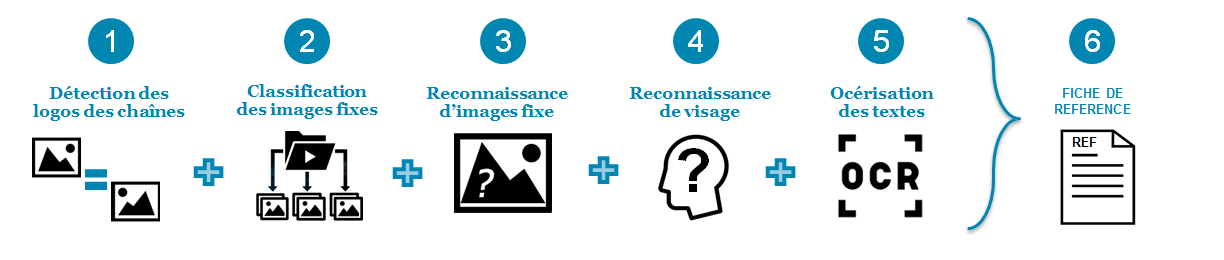
\includegraphics[width=0.8\textwidth]{images/image11.png}
	\caption{Les traitements effectués par l'INA sur une image}
	\label{fig:image11}
\end{figure}


\begin{center}
	Depuis \enquote{L'évolution des pratiques de description des archives...} page 199. 
\end{center}

L’institution a aussi la possibilité d'utiliser les données ainsi organisées pour réaliser des visualisations de données, avoir pris le temps de les structurer rend en effet bien plus aisées et pertinentes ce type de réalisations. En témoigne le projet Data.INA.fr (qui sera évoqué dans notre troisième partie). Les visualisation de données seront ainsi l’objet de notre prochaine partie en tant que nouveau type d'interfaces d'accès au savoir.

\chapter{La visualisation de données en tant que nouvelle interface\index{Interface} au service de la découvrabilité}

\subsection{Voir globalement : l'importance d'avoir une vue d'ensemble des collections}


Comme décrit plus haut, la digitalisation du patrimoine a créé des volumes de données immenses et a, dans le même temps, changé notre rapport au patrimoine qui est devenu plus intangible\footcite[p. 1]{windhager_visualization_2019}, plus « virtuel ». Aux salles de lecture d’archives saturées des années 1980, ont succédé des sites web qui le sont tout autant — si ce n’est plus. Dans le cas du patrimoine audiovisuel, massivement numérisé dans les années 2000 comme décrit, les interfaces sont très souvent les seuls moyens d’accéder aux objets patrimoniaux. Cette nouvelle approche d’un patrimoine intangible, accessible par le biais d’interfaces web basées sur les métadonnées, change les pratiques et usages, notamment le sens de recherche. Là où les chercheurs démarraient aux niveaux hiérarchiques hauts (fonds, collections, etc.), les moteurs de recherche donnent aujourd’hui accès au niveau de la pièce directement, rendant difficile l’appréhension des collections dans leur ensemble et rejoignant le concept déjà décrit de « fatigue muséale\index{Fatigue muséale} »\footcite[pp. 62-72]{gilman_museum_1916}. Les interfaces web classiques : une barre de recherche et des filtres à facettes viennent reproduire, et même amplifier, cette problématique de fatigue muséale\index{Fatigue muséale} ; les utilisateurs occasionnels étant souvent confrontés à un syndrome de la barre de recherche blanche. Sans vue d’ensemble sur les fonds, ils ne sont pas capables d’aller les explorer. C’est pourquoi, le concept d’interfaces dites généreuses est né\footcite[pp. 5-6]{windhager_orchestrating_2018}, elles partent du postulat que l’utilisateur n’est plus un chercheur en manque d’information, mais un flâneur qui souhaite découvrir le fonds. La priorité de telles interfaces, contrairement aux barres de recherche qui favorisent la « trouvabilité\index{Trouvabilité} », est de favoriser la découvrabilité\footcite[p. 18]{shen_generous_2023}. La visualisation de l’information (ou \textit{data visualization}) prend alors une importance nouvelle puisqu’elle peut permettre de réduire cette fatigue muséale\index{Fatigue muséale} tout en améliorant la découvrabilité des fonds.

Prenons ici comme exemple l’expérience conduite par le laboratoire de recherche de la bibliothèque publique de New York « le catalogue\index{Catalogue} en réseau »\footcite[§20 à §26]{lapotre_visualiser_2016}, dont l’objectif était de montrer la totalité du catalogue\index{Catalogue} sur une seule image et de voir les relations qu’entretiennent les objets entre eux, comme si le catalogue\index{Catalogue} avait un bouton « voir tout »\footcite{miller_networked_2014}.


\begin{figure}[h!]
	\centering
	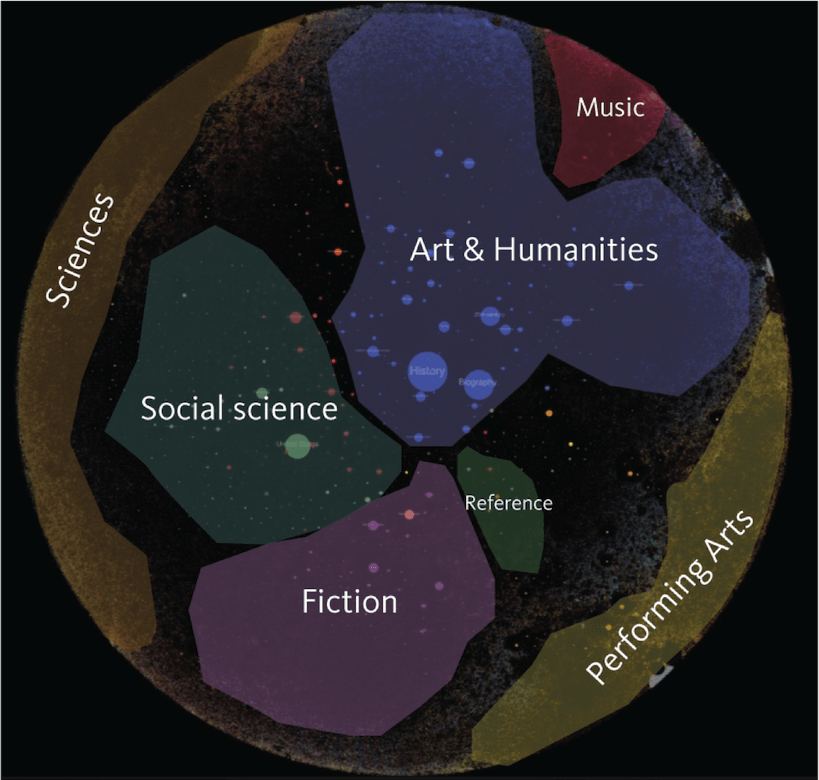
\includegraphics[width=0.6\textwidth]{images/image12.png}
	\caption{Les grandes thématiques qui se dégageant de l'expérimentation de la bibliothèque publique de New York}
	\label{fig:image12}
\end{figure}

\begin{center}
	Depuis \enquote{The networked catalog}, Miller...
\end{center}


Techniquement parlant, cette visualisation utilise les descripteurs \textit{MARC} d’indexation de chaque item et les affiche sous forme de points colorés : plus un point est gros, plus il y a d’ouvrages le concernant dans la bibliothèque publique de New York ; si deux sujets sont souvent mentionnés ensemble, par exemple Jeux-Olympiques et sport, on en déduit qu’ils sont liés d’une manière ou d’une autre et ils se voient attribuer la même couleur.

Outre le fait qu’elle soit fascinante et que l’explorer et s’y perdre soit passionnant\footnote{La navigation interactive est disponible en suivant ce lien : \url{ http://catalog-network.s3-website-us-east-1.amazonaws.com/}}, elle permet, d’un coup d’œil, de se rendre compte des pans de la collection très représentés et centraux ainsi que des liens sémantiques, parfois étonnants entre des entités. Cela permet de se rendre compte de ce qu’une bibliothèque, en tant que réceptacle du savoir à un instant donné, conserve le plus. La visualisation peut donc être, comme l’écrit Raphaëlle Lapôtre, « un moyen heuristique qui participerait à la production de connaissances »\footcite[§ 23]{lapotre_visualiser_2016}. En plus de donner une vision d’ensemble et de favoriser la compréhension globale de la collection, elle permet de révéler de nouveaux aspects. On serait évidemment tenté de voir dans cette image une visualisation des connaissances, comme si une bibliothèque était le reflet du réel et des connaissances produites, mais il est déformé : parce que le contenu d’une bibliothèque est le reflet des politiques documentaires de son époque ; parce que les données ne sont pas si fiables, qu’elles sont truffées d’erreurs humaines ; de choix d’indexation ; des migrations de données et des changements de vocabulaires. Par exemple, le mot tsunami n’est employé que depuis récemment, on lui a longtemps préféré « raz-de-marée »\footnote{Propos rapportés par Denise Barcella}.

Éclairons notre propos avec l’exemple de la RTS où l’on a voulu effectuer une démarche similaire pour proposer un outil de navigation sous forme de \textit{treemap} hiérarchique en utilisant les codes contenus, métadonnées fournies pour chaque document renseignant sa thématique de façon hiérarchique, par exemple un téléjournal sera classé sous actualité.



\begin{figure}[h!]
	\centering
	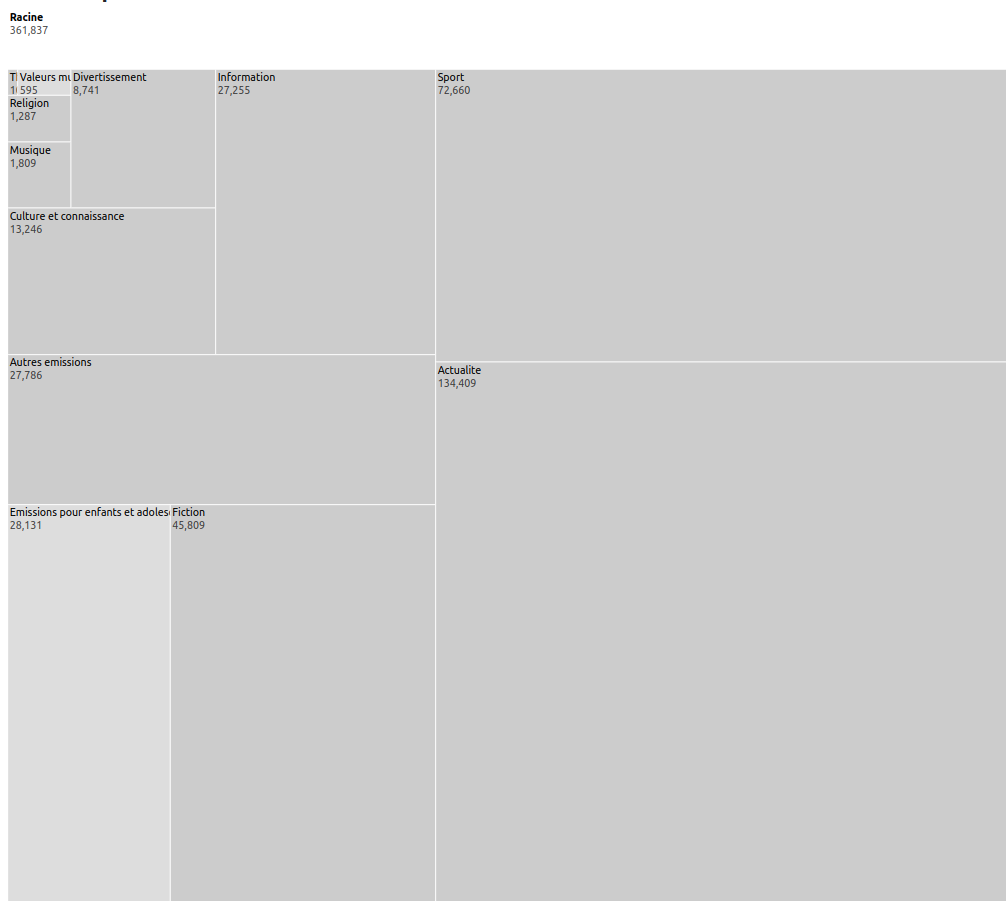
\includegraphics[width=0.8\textwidth]{images/image13.png}
	\caption{Treemap interactive réalisée pendant le stage}
	\label{fig:image13}
\end{figure}



Une fois la visualisation réalisée, nous nous sommes rendu compte qu’elle n’était absolument pas le reflet de ce qui était conservé à la RTS. D’abord, car seule une petite proportion des documents avait un code contenu renseigné (361 837 documents), ensuite car ce qui fait varier la taille des rectangles, le nombre d’items, ne reflète pas la réalité : il n’y a pas plus de sport que de fiction diffusée, c’est simplement qu’on conserve et indexe rarement la fiction qui est souvent achetée en externe. Par ailleurs, on retrouve énormément d’actualité, ce qui est en partie vrai, mais elle est aussi beaucoup représentée, car c’est la seule, depuis les années 1980, à être archivée de façon systématique. Comme la carte de la bibliothèque publique de New York était plus le reflet de son histoire institutionnelle et documentaire, cette visualisation est le reflet des pratiques documentaires de la RTS plus que de ce qui est conservé en son sein. Dans les deux cas, surtout à New York, l'objectif de donner une vision d'ensemble de la collection semble accompli. Les possibilités heuristiques offertes par la visualisation de données, une fois les spécificités et biais potentiels pris en compte, sont prometteuses. En effet, cela permet d'envisager de fournir aux utilisateurs des collections des clés de lecture\index{Clé de lecture} différentes, qui feront l'objet de notre prochaine partie.

\subsection{Voir sous un autre angle : donner des clés de lecture différentes des collections}

On vient de voir que la visualisation de l’information, en plus d’offrir une indispensable vue d’ensemble des collections, offre un potentiel heuristique nouveau. Elle permet en effet « d’opérer un “point de vue” sur un sous-ensemble de résultats pertinents afin d’en faciliter la compréhension »\footcite[§ 3]{hachour_fouille_2015} ; l’intérêt de visualiser des données est donc d’offrir aux regardeurs différentes clés de lecture\index{Clé de lecture}\footnote{ « Concept ou angle d’approche permettant de comprendre, d’analyser, d’interpréter ou encore de critiquer un texte, une œuvre, ou un phénomène. » - Wikictionnaire } d’une collection. On peut séparer ces clés de lecture\index{Clé de lecture} en trois catégories (qui peuvent se cumuler) : vues multiples (listes, mosaïques, etc.) ; encodage spatial (cartes géographiques, diagrammes de réseau, etc.) et encodage temporel (frises chronologiques, animations)\footcite[p. 76]{windhager_review_nodate}. À chaque catégorie correspondent des possibilités interprétatives différentes, par exemple : un diagramme en réseau permet d’explorer la proximité entre des objets culturels, une animation temporelle permet de donner à voir les évolutions temporelles des objets\footcite[p. 77]{windhager_review_nodate}.

La multiplication des interfaces de visualisation offre aux utilisateurs un accès riche et non restrictif aux collections culturelles, ce qui permet d’explorer des ensembles de données vastes. Ce faisant, ces différentes interfaces sont des outils précieux pour exposer la richesse et la diversité des collections culturelles afin que les utilisateurs puissent naviguer entre différentes perspectives. Pour les qualifier, F. Windhager et al. parlent d’« interfaces généreuses ».\footcite[p. 5]{windhager_orchestrating_2018} qui se distinguent des interfaces classiques par une capacité à présenter de grandes quantités d’informations en soutenant les utilisateurs dans leurs tâches cognitives afin de limiter la fatigue. De même qu’un bâtiment doit être généreux et offrir des espaces vides et des plafonds hauts pour être agréable à utiliser, les interfaces, en tant que substituts théoriques, doivent faire de même.

Elles doivent donc être conçues pour éviter la surcharge cognitive en offrant des représentations multiples des données, ce qui permet aux utilisateurs de construire une vision globale et cohérente des collections qu’ils explorent\footcite[pp. 5-6]{windhager_orchestrating_2018}. Elles se veulent des « anti barres de recherche », car, selon les auteurs, ces dernières sont construites selon deux suppositions préalables : le visiteur connait, au moins vaguement, ce qu’il cherche et il ne souhaite pas « s’engager dans la complexité de l’espace de recherche qui leur est caché »\footcite[p. 6]{windhager_orchestrating_2018}.

Afin d’illustrer notre propos, nous mettrons en parallèle un exemple issu d’une réalisation pendant le stage (carte interactive des contenus archivés par la RTS) et le tableau de bord réalisé par la Bibliothèque du Congrès pour visualiser la presse numérisée\footcite[tableau de bord accessible en suivant l'url suivante \url{https://public.tableau.com/app/profile/chronicling.america/viz/ChroniclingAmericaTemporalCoveragebyStateMap/TemporalStateCoverage}]{noauthor_chronicling_nodate}.

D’abord, donc, la carte interactive des contenus (visible en page suivante) qui se présente, comme son nom l’indique, sous forme d’une carte de la Suisse avec la possibilité de naviguer entre les différents niveaux territoriaux du pays : cantons, districts et communes. Elle permet, en un seul regard, d’observer les territoires pour lesquels la RTS conserve le plus d’archives et de cliquer sur ces derniers pour consulter les archives qui s’y réfèrent. Elle combine les niveaux de lecture spatiaux et temporels décrits plus haut en permettant aux utilisateurs de naviguer dans le temps pour observer les variations dans la collection. Par ailleurs, ils ont la possibilité d’inclure un terme de recherche pour observer la répartition géographique de ce terme. Par exemple, dans l’image ci-après, on a tapé « abricots » et on observe que le canton le plus représenté est le Valais\footnote{Canton produisant 90 \% des abricots Helvètes}. Cette carte n’est donc pas uniquement un outil d’exploration, elle permet aussi de réaliser des statistiques à partir des recherches effectuées en proposant un export (au format Excel) de ce qui est visualisé. L'image est ici synoptique, elle permet de voir plusieurs temporalités et états dans le même temps, c'est un choix sémantique fort mais qui peu parfois être complexe pour l'utilisateur, c'est pourquoi d'autres projets préfèrent scinder les possibilités heuristiques en plusieurs visualisations. Tel est le cas de la bibliothèque du Congrès et de son tableau de bord (image ci-après.)



\begin{figure}[h!]
	\centering
	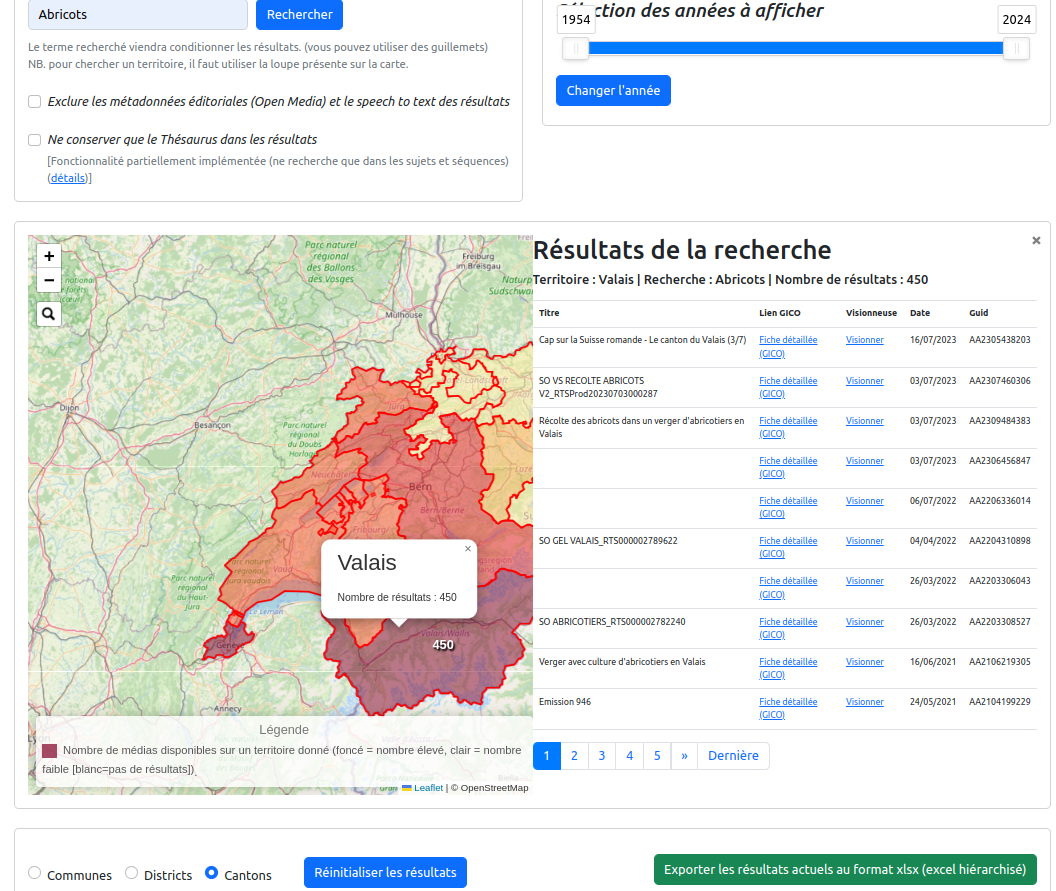
\includegraphics[width=0.6\textwidth]{images/image14.png}
	\caption{Carte interactive des contenus archivés à la RTS réalisée pendant le stage}
	\label{fig:image14}
\end{figure}


L'instutitution propose en effet un tableau de bord, lui aussi interactif. Il permet aux utilisateurs de voir le nombre de journaux numérisés disponibles dans chaque État. C’est là aussi une interface\index{Interface} qui combine une lecture spatiale et temporelle, mais, ici, le choix a été fait de séparer ces deux clés de lecture\index{Clé de lecture}, la carte permet de sélectionner l’État pour que l’utilisateur puisse visionner le nombre de titres de presse disponibles et numérisés à travers le temps. Cette interface\index{Interface} ne permet, en revanche, pas de consulter directement les titres de presse.


\begin{figure}[h!]
	\centering
	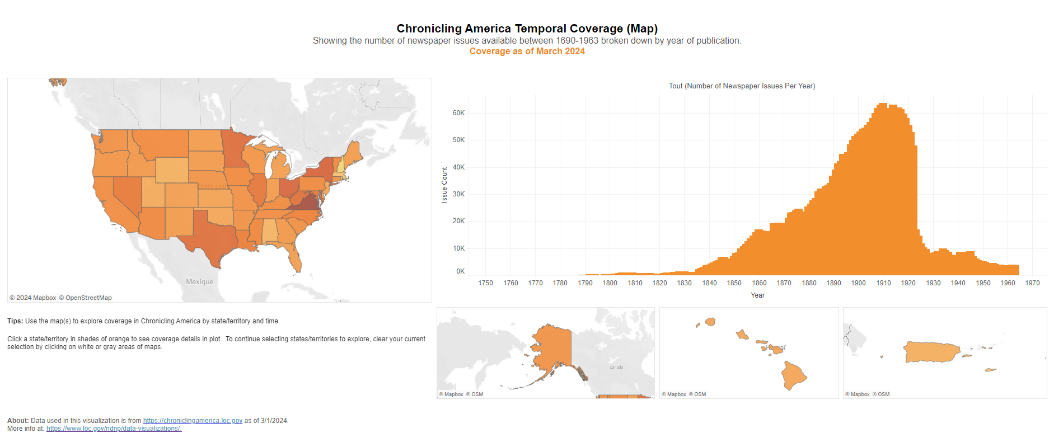
\includegraphics[width=0.8\textwidth]{images/image15.png}
	\caption{Tableau de bord \enquote{Chronicling America Maps and Visualizations}}
	\label{fig:image15}
\end{figure}


On a donc ici deux approches similaires, mais avec des visées différentes, la première approche est plus du côté de l’interface\index{Interface} de navigation dans les collections, la seconde est statistique. Dans les deux cas, on offre aux utilisateurs la possibilité de voir dans son ensemble un fonds extrêmement volumineux en proposant des clés de lecture\index{Clé de lecture} variées. Soit elles sont combinées dans une seule visualisation à l’aide de filtres, soit elles sont séparées en deux visualisations différentes. Cette vision d'ensemble permet aux personnes consultant les fonds de ne pas tomber dans certains écueils. Par exemple, dans le cas de la RTS, étant une chaîne romande, la majorité des sujets concerne la région linguistique francophone. Si l'on souhaite effectuer une recherche sur des cantons italophones ou germanophones, ce ne sera pas l'endroit le plus pertinent. Ce type d’interface\index{Interface} répond donc à de multiples problématiques : donner une vision d’ensemble et des clés de lecture\index{Clé de lecture} différentes d’un fonds ; permettre une interprétation quantitative ; être utilisé dans des actions de valorisation tout en limitant le syndrome de la barre de recherche blanche décrit plus haut. Par ailleurs, la multiplicité des filtres permet une granularité de navigation très importante donnant de nombreuses opportunités de se concentrer sur des documents spécifiques\footcite[p. 7]{windhager2018a}. Combiner différentes clés de lecture\index{Clé de lecture} (dans le cas de la RTS, nous avons ajouté à cette visualisation un \textit{knowledge graph\index{Knowledge graph}} visible plus bas) en prenant en compte le fait que chacune permet de capturer un aspect spécifique de la collection est donc une stratégie intéressante dans le cadre d’objets culturels complexes. Par ailleurs, cela permet de créer des possibilités pour les utilisateurs de faire des découvertes par sérendipité\index{Sérendipité}, car ce type d’interface\index{Interface} les laisse « flâner » dans les collections comme le notent Thudt et al.\footcite[(cité dans)]{windhager2018a}. En revanche, comme le notent Florian Windhager et al., réaliser des interfaces généreuses combinant de nombreuses visualisations et possibilités de filtrage peut recréer la problématique de fatigue muséale\index{Fatigue muséale} citée plus haut en créant ce que les auteurs appellent le « split attention challenge »\footcite[p. 9]{windhager2018a}. Les interfaces, de même que les bâtiments, doivent donc, tout en restant généreuses, ne pas proposer trop de niveaux de lecture et rester simples d’utilisation, car dans les deux cas, cela résulte en un usager perdu : dans l’immensité de l’espace physique ou virtuel (ici aussi, le site François-Mitterrand est éclairant).

\begin{figure}[h!]
	\centering
	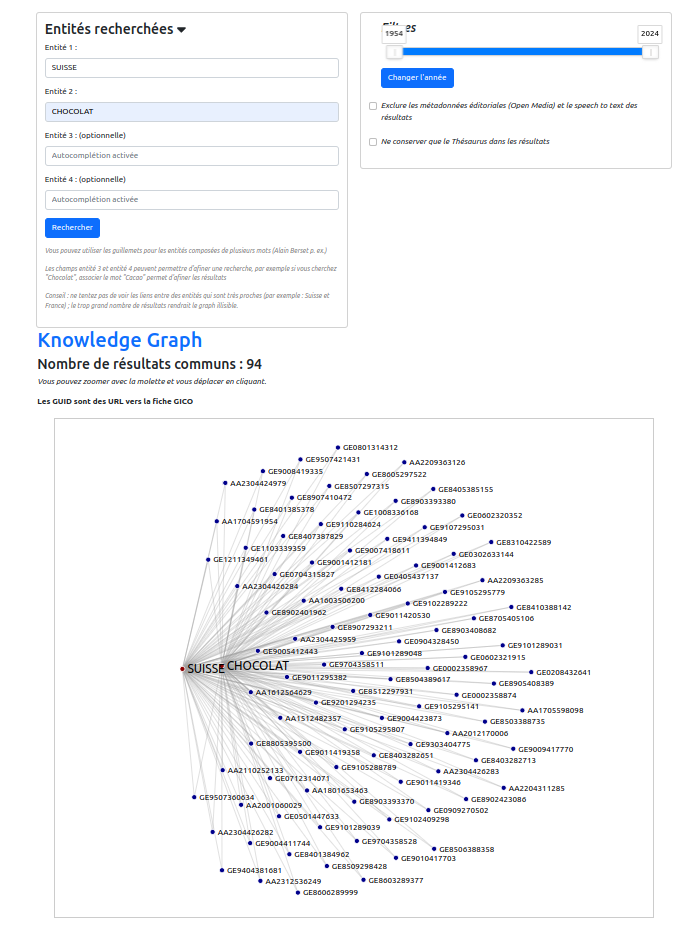
\includegraphics[width=0.6\textwidth]{images/imageknowledge.png}
	\caption{\textit{Knowledge Graph\index{Knowledge graph}} réalisé pendant le stage}
	\label{fig:imageknowledge}
\end{figure}


\subsection{Voir pour aller plus loin}

Dans la partie précédente, nous avons montré que les interfaces pouvaient permettre de se substituer aux bâtiments en proposant une vue d’ensemble des collections et une navigation dans cette dernière, à la manière des déambulations dans un lieu physique. Mais les interfaces peuvent-elles permettre d’aller plus loin ? Peuvent-elles permettre de dépasser les capacités humaines en matière de découvrabilité ? Pour tenter de répondre à ces questions, nous allons explorer le projet de recherche Philherit présenté lors de la journée d’étude organisée par la Bibliothèque nationale de France le 20 juin 2023 « penser la découvrabilité des contenus culturels »\footcite{plouviez_philosophie_2023} et le projet \textit{Impresso} (projet d’exploration de corpus de la presse écrite [images et textes])\footcite{noauthor_impresso_nodate}.

Comment poser la question de l’héritage dans le domaine de la philosophie de nouveau ? C’est la question que pose le projet Philherit. Pour y répondre, le corpus à analyser est extrêmement vaste, car la question était centrale au XIXe siècle\footcite{plouviez2023} du fait de sa proximité avec les questions de justice sociale entre autres. Ce corpus se constitue, par ailleurs, de sources très variées (périodiques, livres, journaux, etc.) et dans toutes les disciplines (économie, philosophie, etc.) réparties en sept bases de données textuelles extraites depuis Gallica. Le texte est ensuite réparti en différents thèmes identifiés par trois mots-clés grâce à l’intelligence artificielle\index{Intelligence artificielle} (\textit{BERT})\footnote{En traitement automatique du langage naturel, BERT, acronyme anglais de Bidirectional Encoder Representations from Transformers, est un modèle de langage développé par Google en 2018 - Wikipédia}. Ce qui est intéressant ici, pour revenir à la question des interfaces, c’est la mise en place d’un nuage de mots qui reprend les thèmes générés par l’intelligence artificielle\index{Intelligence artificielle} et les donne à voir de façon synthétique : plus un mot sera gros, plus il sera représenté dans le corpus, ce qui permet de dégager de grands thèmes et d’aller consulter les ouvrages essentiels\footnote{Il nous a été impossible de trouver une image de bonne qualité de cette interface\index{Interface}, elle est tout de même visible dans la vidéo suivante : \url{https://youtu.be/4zaebvULdc4?t=4787} à 1h19 et 47 secondes.}. Mélanie Plouviez, dans son intervention, dégage trois impacts de l’utilisation des interfaces pour l’amélioration de la découvrabilité du corpus : premièrement, l’accélération de l’analyse, qui était avant réalisée sur \textit{Excel} manuellement et est désormais possible d’un seul coup d’œil sur l’interface\index{Interface} ; deuxièmement, l’amélioration de l’analyse dite « hypertextuelle », c’est-à-dire de l’exploration des liens entre les documents ; et, troisièmement, l’amélioration de la sérendipité\index{Sérendipité}\footcite{plouviez2023}. La chercheuse conclut son intervention en citant Michel Foucault qui, dans son \enquote{archéologie du savoir}\footcite{foucault_archeologie_2008}, définissait les archives comme une « masse discursive » à laquelle les humanités numériques auraient mis fin tout en permettant de faire émerger de multiples points de vue d’une même collection grâce à diverses interfaces\footcite{plouviez_philosophie_2023}.

Les interfaces permettent-elles de dépasser les capacités humaines uniquement dans le cadre de projets spécifiques et de cas d’usages précis ? Attardons-nous sur le projet \textit{Impresso}, dont l’objectif est d’améliorer la découvrabilité de la presse numérisée suisse et luxembourgeoise (donc en 4 langues). Il est mené par une équipe interdisciplinaire d’historiens, linguistes et informaticiens ainsi que des designers — essentiels pour la réalisation d’interfaces efficaces\footcite{ehrmann_explorer_2021}. Ici, en plus de répondre à des cas d’usages « de chercheurs », le projet tente d’être accessible et utile pour les non-spécialistes en répondant à cinq cas d’usages : récupération du contenu utile, compréhension et contextualisation, comparaison des résultats, exportation pour analyse et transparence (documentation du code) et explicabilité de ce dernier\footcite[pp. 5-7]{during_transparent_2024}. L’interface\index{Interface} répond donc à ces cas d’usages en offrant, entre autres choses\footnote{Nous ne décirons pas ici toutes les fonctionnalités, ce serait trop fastidieux.}, la possibilité pour ses utilisateurs, une fois un terme recherché, de compléter leur recherche. Soit de façon thématique, avec des personnalités liées, ou bien des collections liées ; sans tenir compte de la langue de leur recherche.

\begin{figure}[h!]
	\centering
	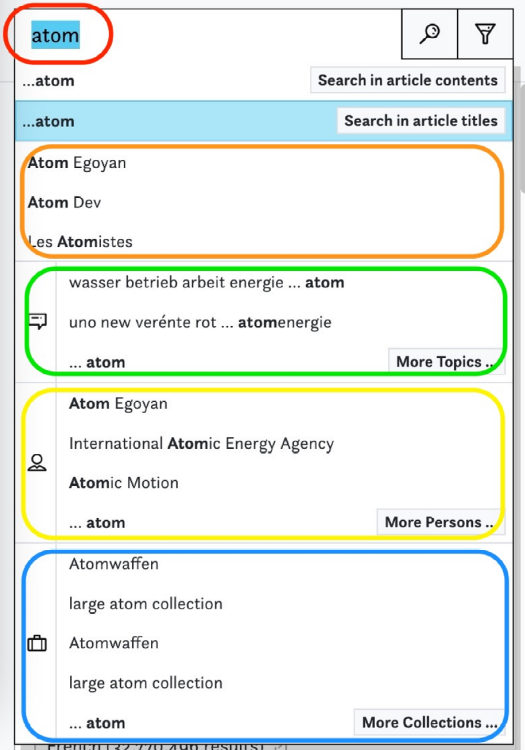
\includegraphics[width=0.3\textwidth]{images/image16.png}
	\caption{Illustration de l'autocomplétion des recherches, depuis \textit{Düring, Bunout, Guido...}}
	\label{fig:image16}
\end{figure}
\newpage

Elle permet aussi de voir les textes et images similaires pour un sujet donné et de voir sa distribution dans le temps en suivant le principe des \textit{n-grams}\footnote{ Un n-gramme est une sous-séquence de n éléments construite à partir d'une séquence donnée - Wikipédia. }. Enfin, elle permet de comparer différents résultats pour observer leur traitement dans la presse. Par exemple, on peut choisir d’observer les résultats communs entre « abricots » et « Valais », et on se rendra compte que l’année du pic observé (1953) correspond à la « révolte des abricots »\footcite{noauthor_revolte_2018}.

\begin{figure}[h!]
	\centering
	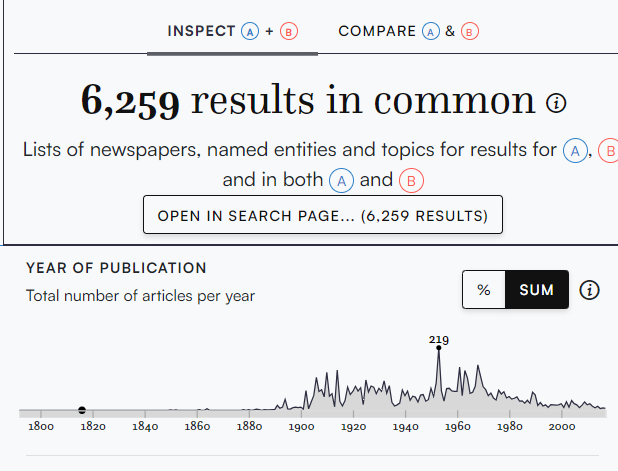
\includegraphics[width=0.6\textwidth]{images/image17.png}
	\caption{Recherche comparative entre \enquote{abricots} et \enquote{Valais}}
	\label{fig:image17}
\end{figure}

Il semble, à en lire les évaluations des utilisateurs, que les fonctionnalités proposées et l’interface\index{Interface} soient non seulement faciles d’accès, mais permettent en outre une grande finesse dans l’exploitation de ce type de corpus textuel. Par ailleurs, les auteurs concluent en énonçant le fait que les chercheurs déjà habitués aux recherches « \textit{data-driven} » étaient très positifs sur les possibilités d’export et d’exploitation offertes, de même que les utilisateurs moins connaisseurs\footcite[pp. 5-7]{during_transparent_2024}.

Au regard de ces deux exemples, on peut noter que la création d’interfaces généreuses tout en permettant de dépasser les capacités humaines des chercheurs (Philherit l’a bien montré) peut aussi être un excellent vecteur de valorisation des collections pour le grand public. Il semble donc que la création de tels outils pourrait être placée du côté des institutions, car, et \textit{Impresso} le montre bien, s’ils sont bien faits et offrent de nombreuses possibilités allant de la plus simple : faire une recherche, à la plus complexe : exporter les données d’une visualisation au format \textit{JSON}\footnote{JSON, pour javascript object notation est un format communément usé pour l'échange de données sur le web} pour les exploiter, ils servent des publics très divers et permettent d’éviter aux chercheurs de créer, de leur côté, des outils dédiés. Ils peuvent alors réutiliser ceux proposés par les institutions pour servir leur cas d’usage ou les réadapter en utilisant les données fournies. Les auteurs de l’article « transparent generosity » sur \textit{Impresso} notent toutefois un certain nombre de limitations à la mise en place de tels outils : silos institutionnels et d’information (causés par des restrictions légales souvent), doublons et mauvaises qualités des données notamment de l’\textit{OCR}\footnote{Reconnaissance optique des caractères}, mais aussi, manque d’interfaces proposant aux chercheurs de découvrir les fonds pour en tirer d’éventuels questionnements\footcite[pp. 1-2]{during_transparent_2024}. Travailler à la correction de ces limitations, notamment celles concernant les données en elles-mêmes, peut aussi permettre aux institutions de gérer de façon plus efficace leurs fonds en ayant une approche dite \textit{data-driven} comme évoqué plus haut.

\chapter{Nouvelles interfaces : nouveaux usages}

\subsection{À chacun son interface\index{Interface} : l'exemple d'InTaVia}

Comme le rappelait très bien la Bibliothèque nationale de France (BnF) dans sa présentation de la journée d’étude (déjà citée) sur la découvrabilité, le défi pour les institutions patrimoniales est bien souvent de réussir à concilier la trouvabilité\index{Trouvabilité}, c’est-à-dire de laisser à l’usager qui sait ce qu’il cherche la possibilité de le trouver rapidement, et la découvrabilité qui lui permettra de trouver ce qu’il n’a pas cherché\footcite{2023e}. Que peuvent les interfaces pour faire face à cette tension ? Peuvent-elles concilier les différents usages et enjeux ? C’est ce que nous tenterons d’analyser en plaçant notre regard sur le projet \textit{InTaVia} (\textit{In/Tangible Cultural Heritage: Visual Analysis, Curation \& Communication}), débuté en 2020 et financé par la Commission européenne.

Les objectifs du projet sont multiples : d’abord répondre aux enjeux d’atomicité des bases de données patrimoniales sur le web (\textit{InTaVia} est donc un portail\index{Portail}) ; ensuite, faciliter la compréhension globale des objets historiques tangibles avec les données intangibles pour améliorer leur interprétation ; enfin, et c’est ce qui va nous intéresser ici, « comme les besoins de chaque audience varient [cette interface\index{Interface}] devra satisfaire différentes exigences scientifiques et pratiques, mais aussi narratives et esthétiques »\footcite{noauthor_overall_nodate}.

On a donc d’abord des enjeux forts de réconciliation de données provenant de sources très diverses et de repérabilité\index{Repérabilité} que nous laisserons de côté, car nous les avons déjà évoqués, pour nous concentrer sur la conciliation entre les usages des chercheurs et d’un public non expert.

Pour parler de ce sujet, nous nous baserons sur un article écrit par J. Liem et al., « A Workflow Approach to Visualization-Based Storytelling with Cultural Heritage Data »\footcite{liem_workflow_2023} dans lequel ils placent la narration comme une stratégie de \textit{design} essentielle pour que l’information, parfois complexe et plurielle dans le cas du patrimoine culturel, devienne intéressante et attrayante pour son public. Les auteurs rappellent par ailleurs qu’actuellement, les outils permettent soit de faire de la narration (penser aux outils d’expositions virtuelles par exemple) soit de faire de la curation, mais jamais les deux ensemble. Ils distinguent aussi trois étapes dans la création d’une narration : collecte de l’information et organisation, création de l’histoire et mise en forme ; l’objectif d’\textit{InTaVia} est de concilier toutes ces étapes dans le même outil\footcite[introduction]{liem_workflow_2023}.

Pour ce faire, \textit{InTaVia} est structuré comme suit : récupération des données tangibles (objets culturels, collections, etc.) et intangibles (métadonnées sur les objets, biographies) provenant d’institutions variées qui sont ensuite répartis en trois canaux : une base \textit{graph} (\textit{knowledge graph\index{Knowledge graph}}), une base relationnelle où les métadonnées sont agrégées en fonction de l’évènement auquel elles font référence (suivant le modèle \textit{CIDOC-CRM\index{Modèles de données!CIDOC-CRM}}\footnote{Le modèle CIDOC-CRM\index{Modèles de données!CIDOC-CRM} est l'équivalent d'IFLA-LRM\index{Modèles de données!IFLA-LRM} pour les musées}) une base tierce qui tente d’agréger « le reste ». Les données sont ensuite traitées par des outils de traitement du langage naturel (\textit{NLP}) pour en extraire les informations utiles aux visualisations\footcite{noauthor_overall_nodate}. Une fois les données agrégées et traitées, l’outil propose à ses utilisateurs un outil de narration qui se divise en deux parties : d’abord la création des histoires et des visualisations à ces dernières à partir des données provenant d’\textit{InTaVia} directement ou d’imports externes ; ensuite, leur mise en forme à l’aide d’une interface\index{Interface} la plus simple possible, mais non restrictive en suivant les trois types de clés de lectures\index{Clé de lecture} décrites plus haut, pour rappel : vues multiples des objets ; organisation spatiale et organisation temporelle. L’immense avantage est ici que quand l’utilisateur ajoute une entité (par exemple une personnalité) dans son histoire, l’outil lui propose directement les entités potentiellement liées grâce à la structure en \textit{knowledge graph\index{Knowledge graph}}\footnote{Qui fonctionne selon le même principe que celui de Google décrit dans notre partie 1}.


\begin{figure}[h!]
	\centering
	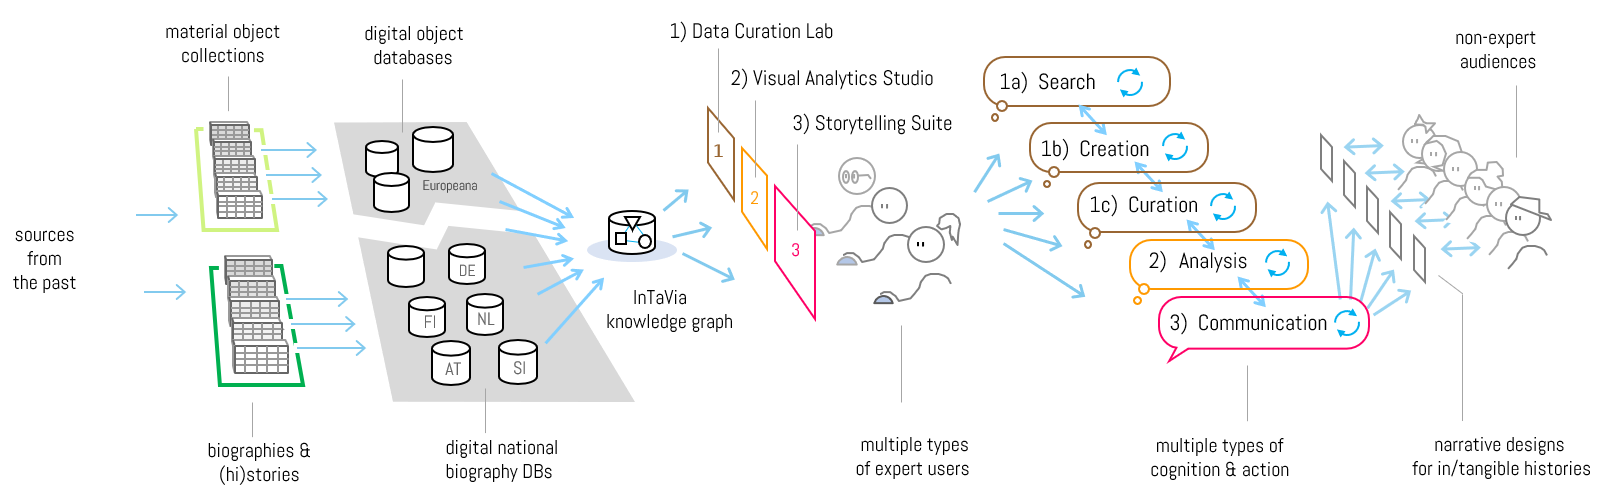
\includegraphics[width=0.8\textwidth]{images/image18.png}
	\caption{Architecture du projet InTaViA}
	\label{fig:image18}
\end{figure}


\begin{center}
	Depuis : Liem, Kusnick, Beck, Windhager, Mayr \enquote{A workflow approach...}
\end{center}

L’interface\index{Interface} d’\textit{InTaVia} (cf. images ci-après) concilie donc tous les usages : de l’utilisateur cherchant à connaitre une thématique particulière, au conservateur de musée souhaitant créer une exposition en ligne en passant par le chercheur souhaitant simplement consulter les collections agrégées. Il parvient donc à concilier la tension entre trouvabilité\index{Trouvabilité} et découvrabilité.


\begin{figure}[h!]
	\centering
	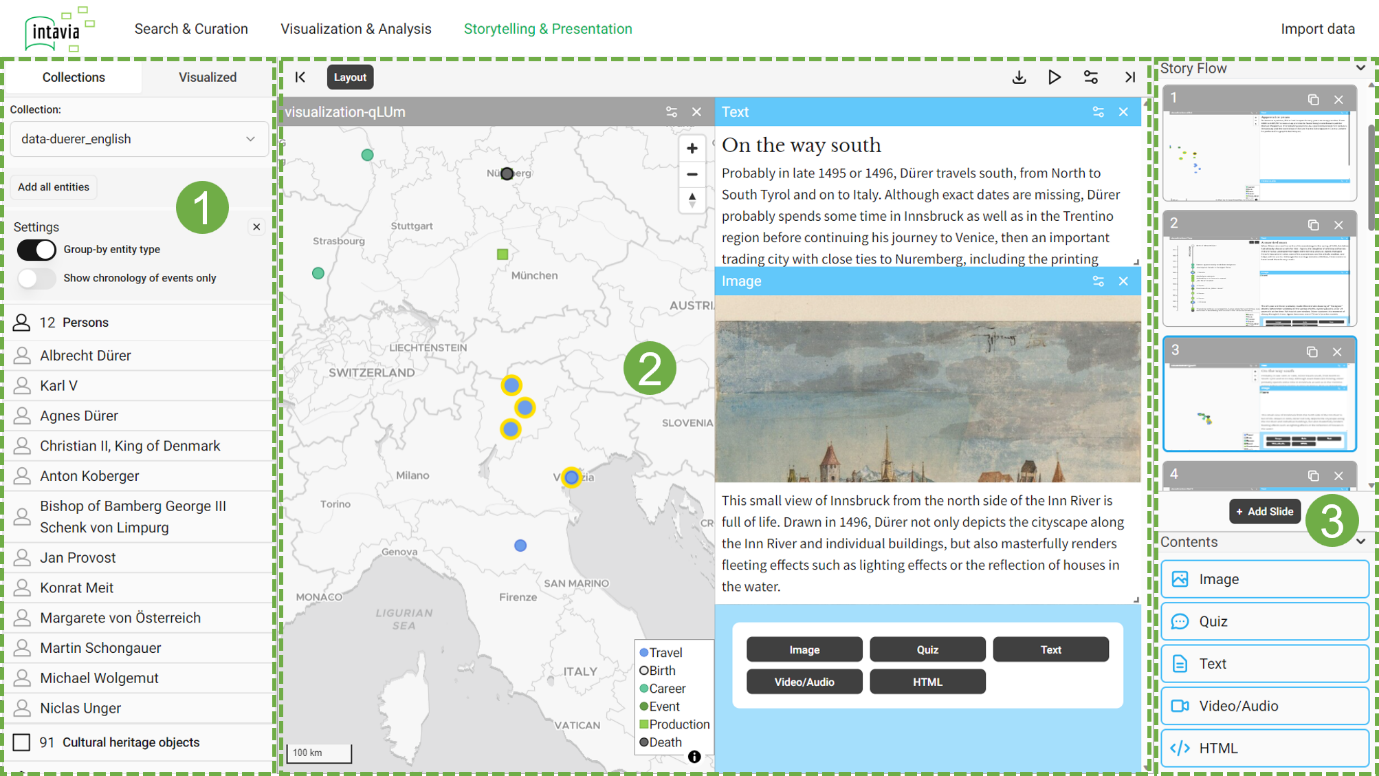
\includegraphics[width=0.8\textwidth]{images/image19.png}
	\caption{L’interface\index{Interface} de création des histoires d'InTaVia}
	\label{fig:image19}
\end{figure}

\begin{center}
	Depuis : Liem, Kusnick, Beck, Windhager, Mayr \enquote{A workflow approach...}
\end{center}




\begin{figure}[h!]
	\centering
	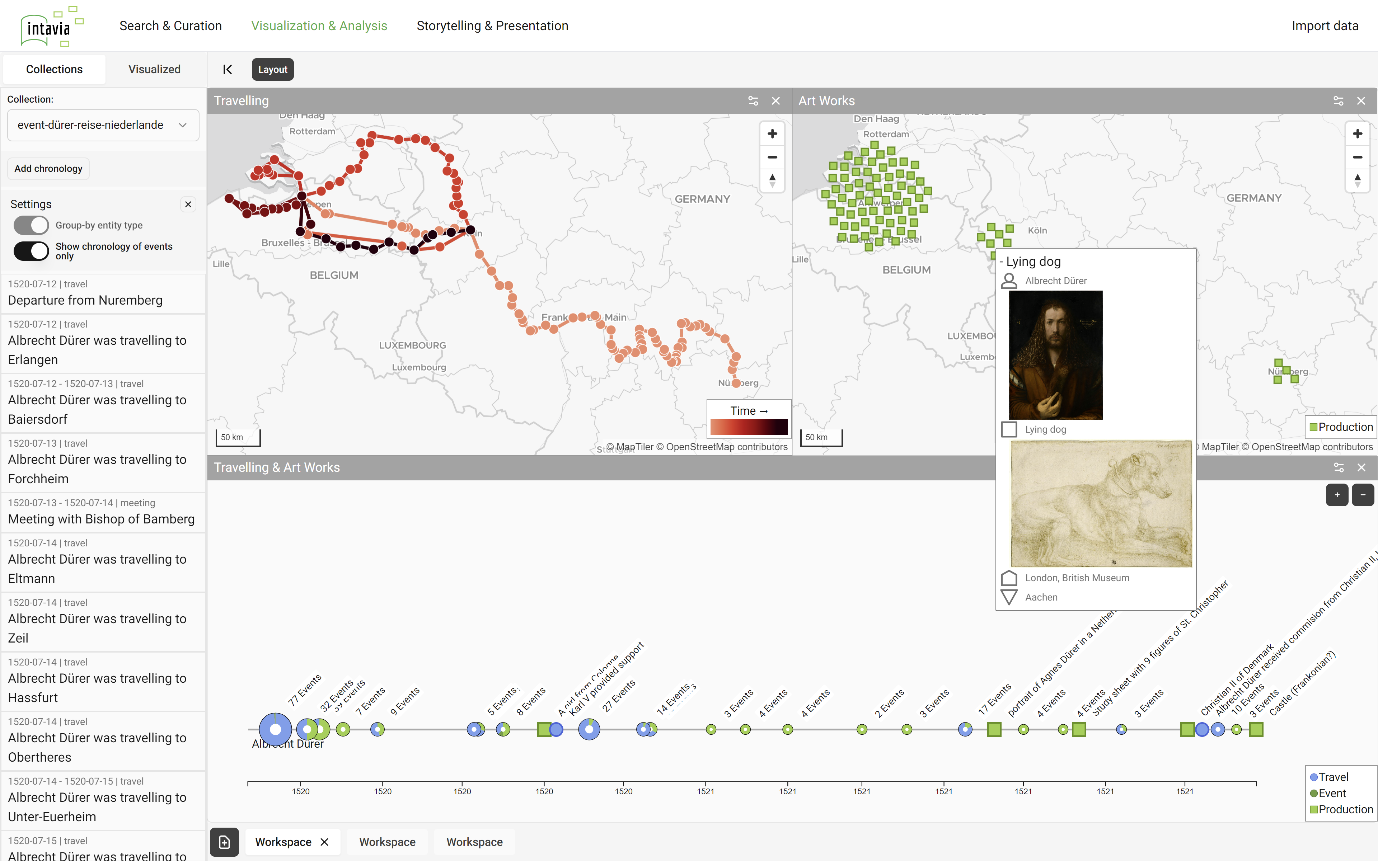
\includegraphics[width=0.8\textwidth]{images/image20.png}
	\caption{Exemple d'histoire créée depuis l'interface d'InTaVia}
	\label{fig:image20}
\end{figure}


\newpage

\subsection{Vers un nouveau \textit{crowdsourcing} reponsant sur l'ouverture des données}


 \enquote{Au Walters art museum, nous avons adopté cette approche [celle de l’\textit{open data\index{Open data}}, N.D.A] et nous avons mis nos manuscrits sur le web pour que tout le monde puisse les voir, toutes les données brutes, toutes les descriptions, toutes les métadonnées, sous une licence \textit{“Creative commons”}. […] Et le résultat, c’est que si vous lancez une recherche d’images dans Google en tapant “Illuminated manuscript Koran”, par exemple, 24 des 28 images que vous obtiendrez viennent de mon institution}\footcite{noel_william_nodate}.

En avril 2012, William Noel, conservateur au Walter Art Museum, consacrait un \textit{TED talk} au \enquote{Codex Perdu d’Archimède en apparence}, mais en réalité, l’acmé de son intervention semble être le moment où il révèle que toutes les données du projet sont en accès libre. Et si l’on regarde la conférence avec cette clé de lecture en tête, on se rend compte qu’elle est parsemée de références à cette notion : des scribes médiévaux copiant les textes antiques, on passe facilement aux internautes créant leur propre collection et s’emparant du patrimoine numérisé. Pour William Noel, non seulement l’\textit{open data\index{Open data}} est \enquote{un avantage pour l’humanité et ce genre de choses}, mais aussi pour les institutions \enquote{parlons de choses égoïstes}\footcite[à 13 minutes 26secondes]{noel_william_nodate}, selon lui : les gens vont au Louvre, car ils souhaitent y voir la Joconde, et ils veulent la voir, car ils la connaissent déjà, car ils ont déjà vu des milliers d’images de l’œuvre : parfois détournées (on pense à l’œuvre de Duchamp\footcite{zotero-368}, mais aussi de façon plus contemporaine aux \textit{memes}\footnote{Concept (texte, image, vidéo) massivement repris, décliné et détourné sur Internet de manière souvent parodique, qui se répand très vite - Larousse}). La constitution de \enquote{communs numériques}\footcite[p. 173]{bermes2024} revêt alors une importance capitale, non seulement dans la préservation, mais aussi dans la transmission\footcite[p. 175]{bermes2024} : permettre aux utilisateurs d’interagir avec le patrimoine (qui doit pour cela être ouvert) fait donc en sorte, entre autres choses, qu’il soit mieux repéré en ligne et plus visionné : car on est beaucoup plus enclin à suivre la recommandation\index{Recommandation} de tiers de confiance (ici, d’autres internautes collaborant au projet) que celle d’une institution\footcite{ertzscheid2019}.

Si nous intitulons cette partie \enquote{vers un nouveau \textit{crowdsourcing\index{Crowdsourcing}}} c’est parce que nous avons observé que la participation en ligne des internautes avait évolué ces dernières années, si avant les activités principales se résumaient plus en un \textit{digital labor} : c’est-à-dire \enquote{la captation de la valeur générée par les activités des internautes en ligne}\footcite{zotero-365} avec des activités qu’Oomen et Aroyo classaient en six domaines en 2011\footcite[(cité par)]{neroulidis_crowdsourcing_2015} : correction/transcription, contextualisation, enrichissement, classification, co-curation et \textit{crowdfunding}. Désormais, les activités en ligne des internautes semblent se tourner vers la notion de communs numériques. On peut exemplifier ce propos avec le site \textit{notrehistoire.ch} lancé en 2009 par la Fonsart\footnote{Fondation pour la sauvegarde de la Radiotélévision, association créée en 2012 par la RTS} avec trois mots d’ordre : publier, participer et explorer\footcite{zotero-361}. Il propose à ses utilisateurs de participer à la création d’un patrimoine commun basé à la fois sur des archives institutionnelles et des archives personnelles. Il est structuré, ainsi que son interface, tel un réseau social en suivant les pratiques du \textit{web 2.0} où l’on peut commenter, créer, partager et publier du contenu en utilisant les archives disponibles sur le site provenant d’une part d’institutions romandes et de l’autre de particuliers. L'interface permet donc de voir des publications d’internautes défiler toujours avec la possibilité d’interagir, on peut aussi choisir d’aller explorer différentes thématiques, voir celles qui sont les plus alimentées, profiter du classement chronologique ou des différents \textit{tags} (identifiés par un dièse dans les publications des internautes).



\begin{figure}[h!]
	\centering
	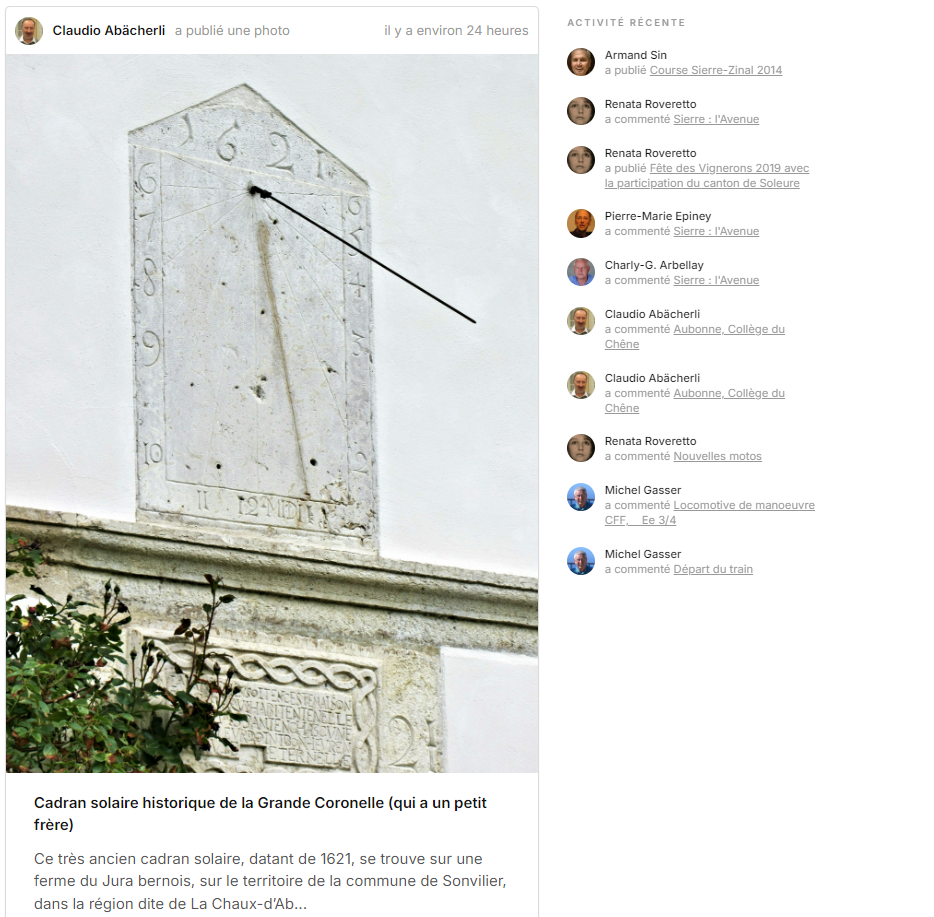
\includegraphics[width=0.8\textwidth]{images/image22.png}
	\caption{L'interface de notrehistoire.ch : un réseau social patrimonial}
	\label{fig:image21}
\end{figure}

\begin{center}
	\url{https://notrehistoire.ch/feed}
\end{center}

Outre le fait qu’il brise les frontières : à la fois physiques entre des documents séparés et organisationnelles, il faut noter que les institutions perdent leur rôle de prescription et deviennent des contributrices à la constitution d’un \textit{Lieu de mémoire commun}\footnote{Toujours en références aux ouvrages parrus sous la direction de Pierre Nora}. Comme Emmanuelle Bermès le rappelle dans son ouvrage : \enquote{leur nouveau défi [des institutions patrimoniales] est d’accompagner et de faciliter l’appropriation du patrimoine numérique par ses communautés bénéficiaires}\footcite[p. 186]{bermes2024}. Même si évidemment, les pratiques de \textit{crowdsourcing\index{Crowdsourcing}} plus classiques identifiées plus haut ne disparaissent pas, il semble que ce nouveau type de pratique, grâce à des interfaces renouvelées, prenne une place de plus en plus importante.


\subsection{L'intelligence artificielle\index{Intelligence artificielle} comme porte d'accès au savoir, encore faut-il trouver la clé}

Précisons ici que nous ne nous concentrerons que sur un seul cas d’usage de l’intelligence artificielle\index{Intelligence artificielle} ici, le \textit{RAG\index{Intelligence artificielle!RAG}} (\textit{retrieval augmented generation}/génération augmentée de récupération), car il nous semble le plus proche de notre sujet de découvrabilité dans le secteur patrimonial. Par ailleurs, nous avons déjà abordé un autre champ d’application de l’intelligence artificielle\index{Intelligence artificielle} dans ce mémoire en parlant d’algorithmes de recommandation\index{Recommandation}.

Comme pour ces derniers, une explication technique est indispensable pour cerner les enjeux autour de cette technologie. Un \textit{RAG\index{Intelligence artificielle!RAG}} est un grand modèle de langue (le plus connu étant \textit{chat GPT}) qui, pour répondre à une question de l’utilisateur (on parle de \textit{prompt}), utilise des données fournies préalablement en tant que source\footcite{pouyllau_quels_2024}. Cette approche combine donc les extraordinaires possibilités des modèles de langues dans la génération de réponses tout en corrigeant leur principal défaut : le manque d’indication des sources et le phénomène d’hallucination\footnote{Dans le domaine de l'intelligence artificielle\index{Intelligence artificielle}, une hallucination ou une confabulation est une réponse fausse ou trompeuse qui est présentée comme un fait certain ; par exemple, un chatbot qui génère un chiffre d'affaires pour une entreprise sans avoir de données à ce sujet. - Wikipédia} ; en somme, leur manque de fiabilité. Pour les fonds patrimoniaux et leur découvrabilité, le potentiel d’une telle technologie est prometteur. Cela améliorerait grandement la recherchabilité en permettant aux utilisateurs de saisir, en langage naturel, leurs requêtes. De l’ère des équations de recherche, nous étions passés aux requêtes \textit{Google-like} avec le \textit{RAG\index{Intelligence artificielle!RAG}}, nous passerions à l’ère du questionnement en langage naturel\footcite{bermes_futur_2024}. Car le changement de paradigme principal de l’intelligence artificielle\index{Intelligence artificielle} dite générative est bien celui-là : ce ne sont plus les humains qui font l’effort de communiquer dans une langue adaptée aux ordinateurs, mais le contraire, ce qui marquerait un « passage de la communication homme-machine à la communication machine-homme »\footcite[p. 7]{pillaud_et_2024}. En termes de découvrabilité, cela signifierait qu’un chercheur/utilisateur du fonds de la RTS (par exemple) pourrait directement demander dans une interface\index{Interface} (souvent un \textit{chatbot} dans le cas du \textit{RAG\index{Intelligence artificielle!RAG}}) « tous les documents concernant l’histoire de la Radiodiffusion en Suisse » dans le fonds de la RTS, ce qui évidemment — outre le fait d’être un immense gain de temps — représente une perspective de recherchabilité incroyable, car une telle requête actuellement ne donnerait que peu de résultats, ce champ n’existant pas dans le thésaurus.


\begin{figure}[h!]
	\centering
	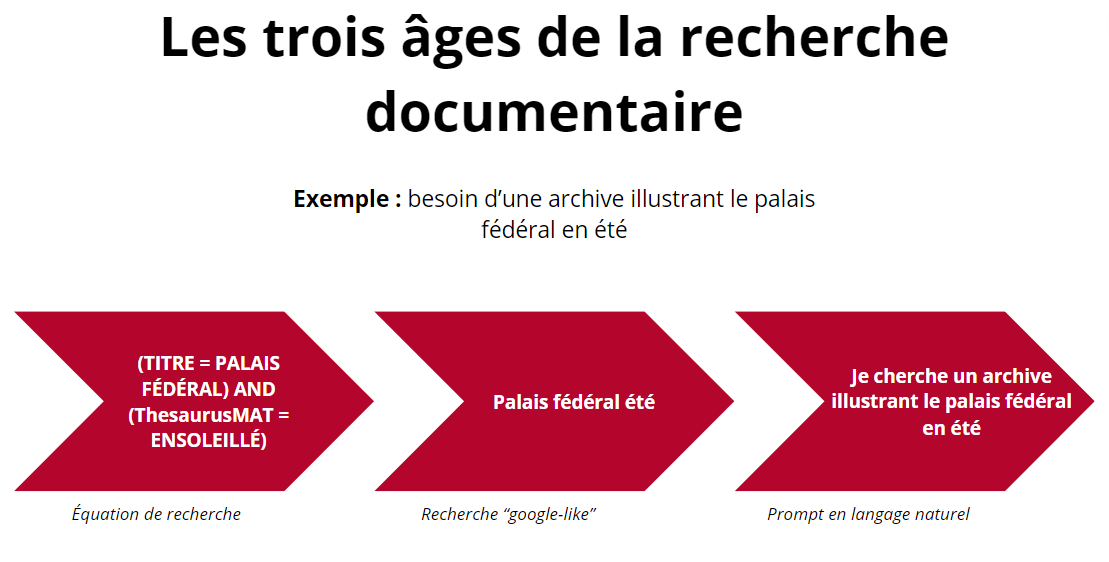
\includegraphics[width=0.8\textwidth]{images/image23.png}
	\caption{Les trois âges de la recherche documentaire, illustration réalisée par nos soins}
	\label{fig:image23}
\end{figure}

Si la mise en place de \textit{RAG\index{Intelligence artificielle!RAG}} peut être vue comme une perspective passionnante pour les acteurs patrimoniaux, il n’en reste pas moins que cela pose de nombreux défis. Défi écologique d’abord (nous le détaillerons dans notre partie 3). Défi éthique et juridique ensuite, la mise en place d’un \textit{RAG\index{Intelligence artificielle!RAG}} nécessite d’utiliser un grand modèle de langue (que les institutions patrimoniales ne développeront jamais en interne) provenant de sociétés privées : Google ou \textit{Open AI} notamment, qui est ensuite adapté (« \textit{fine tuné} ») avec les données internes pour être utilisé. Mais pour faire cela, il faut envoyer les données aux serveurs des entreprises (par le biais d’interfaces de programmation ou \textit{API}), car il est très difficile d’entrainer localement ces modèles qui ont besoin d’une infrastructure importante et ne sont pas \textit{open source}. Même si depuis peu \textit{Open AI} et Google ont indiqué ne pas utiliser les données transférées pour entrainer leurs modèles\footcite{rochefort2023}, ces dernières sont tout de même stockées sur leurs infrastructures ce qui pose des questions de gouvernance de la donnée et de confidentialité en cas d’attaque.

Notons d’ailleurs que pour ces sociétés, les données extrêmement bien structurées des institutions patrimoniales sont véritablement du pain béni, en témoigne le récent partenariat qu’un consortium de trois sociétés spécialisées dans l’intelligence artificielle\index{Intelligence artificielle} générative (\textit{Mistral AI}, \textit{Giskard} et \textit{Artefact}) ont tissé avec la Bibliothèque nationale de France et l’Institut national de l’audiovisuel français\footcite{clavey_bnf_2024}. La BnF précise d’ailleurs : « le monde a redécouvert que toutes les bibliothèques nationales comme la BnF sont des grands réservoirs de données. Le nôtre est probablement le plus grand réservoir de données propres et qualifiées au monde. D’un seul coup, ça intéresse donc nos petits camarades qui travaillent sur l’intelligence artificielle\index{Intelligence artificielle} parce qu’au-delà du logiciel, il faut de la donnée pour les entrainer ». Ces « grands réservoirs » deviendront sûrement un enjeu très important dans les années à venir puisque les besoins en données de l’intelligence artificielle\index{Intelligence artificielle} générative sont de plus en plus importants. Les chercheurs évoquent d’ailleurs la date de 2026 comme celle où toutes les données publiques de l’Internet auront été aspirées par les modèles en formation\footcite{forbes_internet_2024}. Même si beaucoup évoquent la possibilité de former ces modèles par des contenus générés par intelligence artificielle\index{Intelligence artificielle}, il semble que cette piste ne donne pas de résultats très probants (pour l’instant, le domaine étant en évolution constante)\footcite{noauthor_entrainer_nodate}.

Il y a, enfin, un défi de repérabilité\index{Repérabilité}, ces technologies ne font pas de miracles : si une partie du fonds n’a que peu de métadonnées, elle ne sera pas renvoyée. Prenons l’exemple de la RTS ici, on a noté dans notre état des fonds que le sport et les émissions pour enfants ont été peu archivés, et quand c’est le cas avec des métadonnées minimales : si un modèle \textit{RAG\index{Intelligence artificielle!RAG}} est mis en place, ces collections resteront invisibilisées, car mal documentées et en petit nombre. L’exemple de Robert Williams est ici tristement éclairant. En 2020, ce dernier, afro-américain, a été arrêté et a passé trente heures en détention parce qu’un logiciel d’intelligence artificielle\index{Intelligence artificielle} avait confondu sa photographie avec celle d’un voleur de montre\footcite{noauthor_etats-unis_nodate}. Ce que cela vient prouver, c’est que les algorithmes, conçus en grande partie par des blancs, commettent bien plus d’erreurs sur des groupes ethniques moins représentés dans leurs données d’entrainement que ceux majoritaires. (Il y a ici un enjeu d’explicabilité algorithmique que nous traiterons aussi dans notre partie 3).

Au regard de ce qui a été écrit, il est essentiel, avant de se lancer dans la mise en production de \textit{RAG\index{Intelligence artificielle!RAG}} pour des collections patrimoniales, de réaliser un travail en profondeur sur les données et leur pondération. Dans le cas de la RTS, cela passerait par une transcription automatique de tous les programmes et la génération de résumés documentaires pour chacun (en utilisant comme données d’entrainement ceux déjà rédigés) ainsi que de mots-clés documentaires issus des thésaurus. Cela permettra un entrainement plus efficace (avec des coûts environnementaux et financiers réduits), car nécessitant moins d’itérations tout en réduisant les biais d’invisibilisation décrits, car tous les documents seront documentés avec la même précision.

Concluons avec ce qu’écrit Emmanuelle Bermès dans un article de blog : « si ce genre de méthode doit révolutionner à terme la recherche documentaire et voir nos recherches par mots-clés disparaître au profit de \textit{prompts}, comme la recherche par équation a disparu au profit de la recherche plein texte… On a intérêt à comprendre comment elles fonctionnent et à apprendre à les maitriser. Car le \textit{prompting}, c’est comme la recherche documentaire : ça pourrait paraître simple à première vue, mais c’est une compétence de la littératie numérique\index{Littératie numérique} qui ne s’invente pas\footcite{bermes_futur_2024}.

% Import de la partie 2
	

	
	%Document vide aux normes de l'École nationale des Chartes
%Dernières modifications E. Rouquette (12/2023)


\part{Partie 3 : le code c'est la loi, régulations et limites à la découvrabilité}
%\setcounter{chapter}{0} % remet le compteur des chapitre à 1 

\chapter*{\enquote{Le code : c'est la loi}}

Le code, c’est la loi\index{Code is law} : « \textit{code is law} »\footcite[(nous avons consulté la version française disponible sur Framablog)]{lessig_code_2000}. Dans un article paru en 2000, Lawrence Lessig met le doigt sur un enjeu central du web : sa régulation\index{Régulation}. Or, le web, à la différence de nos sociétés, n’est pas régulé par des textes de loi et une constitution : non, ce qui régule le web c’est le code, c’est lui qui détermine s’il est facile ou pas d’accéder à un contenu, qui détermine si vous allez pouvoir découvrir cet incroyable vase grec, c’est lui encore qui décidera de votre orientation (l’exemple de \textit{Parcoursup} le montre). Si les règlements\index{Régulation} européens récents, tel que celui sur la protection des données tentent de réguler le web, force est de constater qu’ils sont limités et ne touchent qu’une infime fraction des interactions que nous avons avec ce dernier. Et comme le montre Laurence Lessig, parfois c’est bénéfique : c’est parce que le protocole \textit{TCP/IP} (qui permet l’échange de données) rend difficile d’associer une adresse IP (celle d’un ordinateur) à une personne que le web est un espace sans précédent de liberté d’expression ; mais c’est aussi pour cette raison que la haine en ligne est difficile à endiguer\footcite[§8 et § 9]{lessig_code_2000}.

Revenons aux origines du web pour comprendre pourquoi l’écosystème a été pensé, dès son origine, de façon si libertaire. Si internet a d’abord été, dans le contexte de la guerre froide, vu comme un moyen de relier de façon décentralisée différents ordinateurs afin d’améliorer la résilience des États-Unis en cas de guerre nucléaire\footcite{2024i}, le projet sera, finalement, surtout utilisé par les universités américaines (en témoigne la première carte du réseau visible ci-après), notamment pour optimiser l’utilisation des très couteux ordinateurs de l’époque.


\begin{figure}[h!]
	\centering
	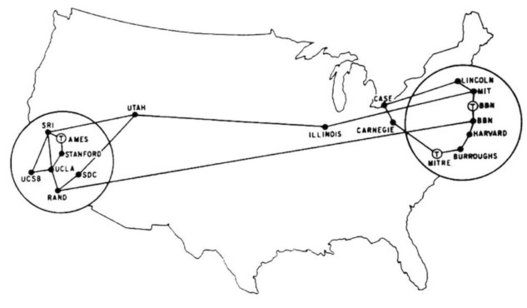
\includegraphics[width=0.8\textwidth]{images/image24.jpg}
	\caption{Carte d’ARPANET en 1972}
	\label{fig:image24}
\end{figure}

\begin{center}
	Depuis : \url{https://www.accessoweb.com/La-carte-de-Arpanet-en-1972-les-debuts-d-Internet_a8123.html}
\end{center}


Les mouvements libertaires, dont Stewart Brand\footnote{ Il est l’objet du livre de Fred Turner, « Aux sources de l’utopie numérique. De la contre-culture à la cyberculture, Stewart Brand un homme d’influence », trad. de l’anglais par Laurent Vannini, Caen, C\&F Éd., 2012, 432 p.}, l’un des pionniers d’internet faisait partie, s’intéressent à cette infrastructure, car ils se méfiaient des structures étatiques centrales et voyaient en internet un potentiel d’interactions libres sans interventions de ces dernières, car il était, dès sa conception, conçu sur un modèle décentralisé. Brand contribue à populariser l’idée que les ordinateurs personnels pouvaient contribuer à l’idéal libertaire en permettant à chacun de devenir autonome au sein d’un réseau mondial sans « tête »\footcite[§ 5]{goeta_fred_2013}.

Mais, pour revenir à l’article de Lessig, si internet et le web ont été pensés dès leurs débuts comme des espaces libres, cette approche n’est pas figée, « car le code n’est pas figé »\footcite[§ 6]{lessig_code_2000}, d’autres éléments peuvent être ajoutés pour permettre d’identifier à coup sûr l’auteur d’une publication par exemple. Comme le code détermine les valeurs d’internet, poursuit l’auteur, c’est en intervenant sur ce dernier qu’on peut les modifier ; il balaye les arguments, très actuels (le patron de X s’en est fait le parangon) selon lesquels on devrait choisir entre une régulation (par l’État par exemple) et son absence : or, le code régule, soit il protège la vie privée soit il promeut la surveillance, soit il laisse la haine en ligne être diffusée soit il tente de la limiter (X est un excellent exemple en la matière). L’auteur conclut son article, écrit en 2000 pour rappel, en expliquant que si l’État n’intervient pas, la régulation\index{Régulation} est placée du côté d’acteurs privés qui ont des objectifs bien différents\footcite[§ 28]{lessig_code_2000}. L’article illustre bien trois enjeux essentiels, que ce soit pour la découvrabilité et la diversité culturelle ou le web en général : le code c’est la loi\index{Code is law} donc il faut comprendre ses biais et problématiques afin de les contrer ; le code c’est la loi donc les institutions doivent s’en emparer, soit pour le réguler, soit pour utiliser son potentiel et ne pas passer à côté ; et enfin, le code c’est la loi donc les personnes qui l’écrivent doivent être conscientes des enjeux que sous-tendent leurs actions. L’objet de cette partie sera donc d’explorer, d’abord les éventuels biais et potentialités du web en matière de découvrabilité, ensuite les questions institutionnelles autour de ce dernier : de la formation des agents à la régulation\index{Régulation}, pour finir, nous nous intéresserons aux angles morts de la notion.

\chapter{Le web : prison ou fenêtre ouverte sur le monde ?}

\subsection{L'hyperchoix\index{Hyperchoix}}

Cette notion est centrale pour commencer cette partie sur le web. On peut la définir comme le fait de faire un choix parmi un grand nombre d’options. Dans son ouvrage « \textit{L’attaque des clones} »\footcite{durand2016}, Emmanuel Durand l’exemplifie avec \textit{Gangnam Style}, vidéo sortie en 2012 et qui en un mois a battu tous les records de visionnages sur \textit{YouTube}, devenant la première vidéo cumulant 1 milliard de vues qui, toujours selon l’auteur, vient révéler deux choses : l’incroyable possibilité de diffusion pour des artistes en dehors des circuits traditionnels et le caractère aléatoire de la notoriété « \textit{buzz} » qui en découle parfois. Pour lui, cette notion illustre le potentiel presque infini du web à se faire diffuseur d’œuvres qui ne l’auraient pas été autrement, dans le monde entier\footcite[§ 1 et § 4]{durand_chapitre_2016}. C’est une révolution : avant l’arrivée d’internet, l’accès aux œuvres de l’esprit était limité, même avec l’émergence, dans le courant des XIXe et XXe siècles des industries culturelles que sont la photographie, la presse ou encore le cinéma ; il était difficile pour des artistes d’acquérir une notoriété et d’être diffusé sans l’appui de grands éditeurs. Internet aurait donc accompli une véritable utopie : celle de l’accès pour tous et toutes (pas totalement, seuls environ 50 \% de la population mondiale ayant accès à internet)\footcite{2024h} à des œuvres et à des savoirs de façon quasi illimitée. Cela contribue, si l’on suit le rapport mondial de l’UNESCO intitulé « \textit{Repenser les politiques culturelles} »\footcite[cité dans Durand Emmanuel, \textit{l'attaque des clones}... § 10]{zotero-651}, à réduire les contraintes : à la fois sociales, géographiques et culturelles au sein des nations tout en ouvrant au niveau mondial le savoir et sa découverte.

Il est vrai que le web ainsi que l’essor de l’informatique personnelle permettent aux créateurs de publier de façon presque gratuite tout en leur donnant la possibilité de créer différemment. Par exemple, nous avons tous la possibilité de nous improviser monteur de vidéos, créateur de musique, illustrateur… Le tout de façon très simple et avec des couts très réduits. Cela a eu pour effet de remettre en cause (au moins en partie) le rôle des industries culturelles et notamment les diffuseurs qui décidaient avant de ce qui serait ou ne serait pas dans le monde culturel\footcite[§ 19]{durand_chapitre_2016}.

Mais cette facilité à publier et à mettre en ligne, et on l’a vu longuement déjà dans ce mémoire, peut aussi être un problème : celui de la masse, comment faire les bons choix ? Comment repérer les Mozart de demain ? Qui plus est quand les choix renvoient à volonté vers d’autres potentiels choix avec le système des hyperliens\footcite{noauthor_hyperchoix_nodate} et à une époque où près de la moitié du trafic mondial serait assuré par des robots et où ils sont en capacité de générer des contenus à volonté\footcite{ertzscheid2023} ?

Il faut donc poser la question de la sélection dans la prescription qui était auparavant la distinction au sein d’une production et qui devient un choix répondant aux attentes d’un consommateur au sein d’une offre pléthorique\footcite{ertzscheid2023}. Mais aussi celle de l’évaluation, qui n’est plus l’avis d’un expert qui désigne une valeur en recommandant ou non un contenu, mais une liste d’avis motivés par des critères, soit qualitatifs, « les plus aimés », soit quantitatifs, « les plus vus ». Car si l’écosystème numérique a permis de court-circuiter les systèmes de diffusion traditionnels, ces derniers n’ont pas totalement disparu et ont été remplacés par des groupes, en immense partie Américains, qui tentent de rassurer leur public avec des « discours d’ONG »\footcite[p. 3]{laugee__2013}, mais qui, quoiqu’on puisse en dire, ont besoin de trafic pour vivre, car ils reposent sur des modèles publicitaires et sur leurs capacités à être prescripteurs, on parle de « capitalisme linguistique »\footcite{kaplan_quand_2011}. C’est-à-dire, qu’au lieu de vendre un produit pour générer des profits, comme c’est le cas de manière classique, ces entreprises, et Google au premier chef, vendent des mots. Ces derniers ont aussi un cours en bourse, ainsi être placé en haut des résultats de recherche concernant le mot « football » sera plus cher pendant la coupe du monde qu’en plein été au moment où les compétitions font une pause (Google Maps fonctionne selon le même principe mais aussi Facebook)\footcite{kaplan_quand_2011}.

On a donc un hyperchoix\index{Hyperchoix} d’une part caractérisé par une quantité informationnelle immense, et de l’autre une « hyperindividualisation »\footcite[p. 3]{laugee__2013} qui vient la canaliser. Au final, la question qu’il convient de poser est celle de la réalité derrière la théorie : est-ce que le web a réduit ou augmenté la diffusion de la culture dans toute sa diversité ? C’est ce que nous tenterons d’observer dans notre prochaine partie en partant du concept de longue traine\index{Longue traine} (\textit{long tail}).

\subsection{Une longue traine ou une courte tête ?}

Le terme de longue traine\index{Longue traine} (\textit{long tail}) a été proposé en 2004 par Chris Anderson qui constatait alors que le web pouvait favoriser l’augmentation de la diffusion des contenus peu ou pas diffusés auparavant : de niche\footcite[§ 8]{benghozi_longue_2008}. Il convient de tenter, après 20 ans, de l’analyser et de l’objectiver, cela nous sera utile pour poursuivre notre réflexion sur l’écosystème qu’est le web et ses spécificités sur le plan de la découvrabilité. Ce que ce terme vient tenter d’exprimer, c’est la grande différence entre l’espace physique, limité, et l’espace numérique qui serait affranchi de toute contrainte spatiale. Pensons à l’exemple d’une librairie : dans un espace donné, elle sera capable d’afficher une vingtaine de milliers d’ouvrages, souvent dans la langue locale\footcite[§ 11 et § 12]{benghozi_longue_2008}. Ce concept repose sur deux effets : une offre qui s’élargit d’une part et de l’autre une recommandation\index{Recommandation} qui devient plus personnalisée, on l’a vu\footcite[§ 17]{bourreau2015a}.

Les chiffres semblent montrer que l’effet \textit{long tail} serait fantasmé et que ce qui serait plutôt mis en place est son exact contraire : l’effet \textit{short head}\index{Courte tête} : la majorité des consultations se feraient sur une partie infime des contenus. On avance souvent la proportion de 80/20 : 80 \% des contenus rassembleraient 20 \% des personnes et 20 \% des contenus 80 \% des personnes\footcite[§ 10]{bourreau2015a}. Il faut cependant nuancer ces chiffres, s’ils restent globalement vrais, il faut tout de même noter que 20 \% des contenus sur le web représentent une diversité bien plus importante que ce qui pouvait être le cas avant l’informatisation : la proportion est restée sensiblement la même, mais elle masque le fait que les chiffres du total de contenus différents consultés ont augmenté de façon très importante\footcite[§ 15]{bourreau2015a}. Dans tous les cas, il est très difficile de conclure à la réalité ou non de cet effet de longue traine\index{Longue traine}, les nombreuses études sur le sujet étant assez contradictoires et très dépendantes du secteur culturel concerné (on évoquera le cas spécifique du patrimoine culturel juste après)\footcite[tableau 1]{bourreau2015a}.

On peut néanmoins tenter, grâce à l’article de Marc Bourreau, Sisley Maillard, François Moreau « Une analyse économique du phénomène de la longue traine\index{Longue traine} dans les industries culturelles »\footnote{déjà cité plusieurs fois} d’expliquer les raisons de la limitation de l’effet \textit{long tail} observées. La première a été formulée par le sociologue MacPhee en 1963 : les gens moins familiers à un marché (par exemple la musique) qui représentent la majorité des consommateurs vont souvent diriger leur choix vers des valeurs plus sûres, déjà bien établies ; les experts, minoritaires, vont eux ventiler leurs choix entre, effectivement, des produits de niches, mais vont tout de même continuer à consommer des produits populaires. Donc in fine, les produits de niches seront plus rarement consultés\footcite[§ 29]{bourreau2015a}. La deuxième raison a déjà été évoquée longuement dans ce mémoire, il s’agit du concept d’économie de l’attention\index{Économie de l’attention}, quand un utilisateur a trop de choix, cela lui demande un coût cognitif élevé, il va donc préférer se tourner par mimétisme, là aussi, vers ce qui lui est soit recommandé : soit par un tiers (ou par son équivalent informatique que sont les classements « titres les plus vus » ou « titres les plus aimés » par exemple), soit par un algorithme (notre prochaine partie sera consacrée à évaluer leur rôle dans les prescriptions culturelles)\footcite[§ 39]{bourreau2015a}. Troisième raison, le manque d’information des consommateurs contribuerait, selon une étude d’Hendricks et Sorensen\footcite[§ 40]{bourreau2015a} (2009) à limiter la visibilité des contenus de niche. Ce qui serait le symptôme visible d’une limite qui reste importante, celle de l’exposition médiatique des titres qui reste réservée à une petite partie des producteurs de contenus culturels, notamment dans les médias traditionnels (limités par leurs grilles) qui conservent toujours un rôle de prescripteurs important\footcite[§ 41]{bourreau2015a}.

Pour revenir au domaine qui nous intéresse, le patrimoine culturel, si les études le concernant sont peu nombreuses et le climat bien moins concurrentiel que celui de la musique par exemple ; on peut néanmoins tirer quelques conclusions grâce à un article paru dans le \textit{Bulletin des bibliothèques de France} (\textit{BBF}) « La découvrabilité des collections numériques patrimoniales sous l’angle des usages de Gallica » (Bastard et Laborderie)\footcite{bastard2023}. Les auteurs y notent que 52 \% de la collection disponible en 2021 n’avait pas été consultée au cours de l’année, ce qui peut paraître important quoique bien plus faible que le ratio de 80/20 évoqué plus haut. Qui plus est, si l’on regarde dans le détail comme le font les auteurs en notant notamment que la presse, qui représente pourtant 76 \% de la collection numérisée, ne représente qu’un cinquième des consultations alors que 79 \% des livres numérisés ont été consultés au cours de l’année. La proportion documents consultés/documents disponibles atteint même 97 \% pour les vidéos et 91 \% pour les cartes\footcite[§ 8]{bastard2023}. Le phénomène de longue traine\index{Longue traine} est donc, semble-t-il, bien plus prégnant dans les usages numériques de Gallica que dans d’autres industries culturelles (les documents les plus consultés ont tout au plus 30 000 visites soit 1 \% du trafic !), et l’on peut tenter de l’expliquer par plusieurs raisons. La première est l’excellente repérabilité\index{Repérabilité} des collections de la bibliothèque nationale en ligne (déjà décrite) qui sont souvent recommandées par les moteurs de recherche (en témoigne l’image ci-après).


\begin{figure}[h!]
	\centering
	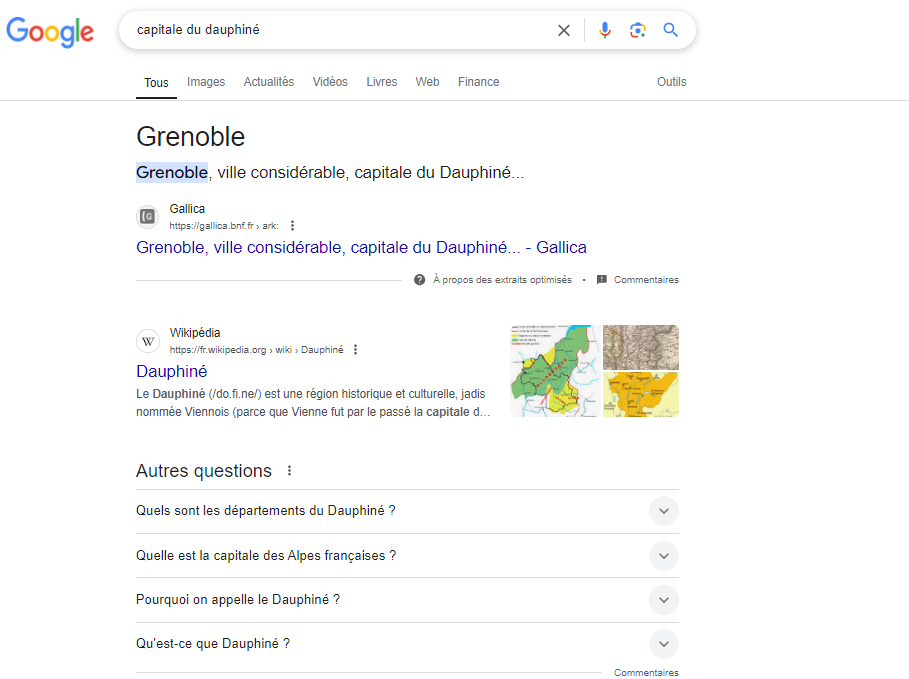
\includegraphics[width=0.8\textwidth]{images/image25.png}
	\label{fig:image25}
\end{figure}



La deuxième raison que l’on peut noter est l’impossibilité pour les utilisateurs de voir les \enquote{documents les plus consultés}, les documents mis en avant sur Gallica le sont par l’équipe éditoriale du site, jamais par rapport à leur audience (impossibilité de l’effet de mimétisme décrit plus haut). Poursuivons avec le fait que Gallica est consultée en majorité par des experts ; de fait, selon une enquête de 2020 menée par l’Observatoire des publics de la Bibliothèque\footnote{ Comme l’écrivent les auteurs, ces résultats ne sont pas forcément le reflet des publics réels de Gallica, mais plutôt de ceux désireux d’améliorer le service et qui le connaissent donc assez bien.} un tiers des usagers du site seraient des chercheurs, un autre tiers serait composé d’amateurs passionnés de science et de savoir (généalogistes, historiens amateurs, etc.) et un autre tiers se répartirait entre professionnels des bibliothèques et visiteurs ayant fréquenté l’établissement, or, comme le montrent les travaux de MacPhee cités plus haut, les experts sont les plus enclins à consulter des contenus « de niche ». Enfin, comme l’exposition médiatique des contenus numérisés dans Gallica est quasi nulle, cela ne contribue pas à en faire émerger certains au profit d’autres. On pourrait se risquer à écrire que la différence fondamentale entre Gallica et les autres industries culturelles qui fait que l’effet longue traine\index{Longue traine} s’observe de façon assez clivante est que le site n’est pas construit selon des logiques marchandes : l’objectif de la bibliothèque nationale n’est ni de vendre de l’espace publicitaire ni de faire rester les internautes sur son site, elle n’a donc aucun intérêt à favoriser un contenu plutôt qu’un autre. En effet, comme évoqué dans l’introduction, si le code est la loi, il s’agit bien de choix de la part des institutions ou des entreprises que de l’orienter vers telle ou telle direction. Nous verrons dans la partie suivante consacrée à la notion de bulle de filtres (et donc à la recommandation\index{Recommandation} algorithmique) que cela s’applique aussi tout à fait.

\subsection{Lutter contre la \enquote{bulle de filtre\index{Bulle de filtre}}}


Depuis quelques années, le phénomène théorisé en 2011 par Eli Pariser de \enquote{Bulle de Filtre}\index{Bulle de filtre} fait énormément parler de lui, il se définit comme un enfermement algorithmique des personnes par le biais d’une personnalisation trop importante. Il nous semble important de revenir en détail sur ce concept, car la découvrabilité est souvent évoquée comme une réponse aux problèmes qu’il pose et qui sont de deux ordres : premièrement un auto-renforcement des opinions politiques et clivages sociétaux, on parle souvent de radicalisation ; et deuxièmement, une perte de diversité culturelle.

Commençons par évoquer le premier cas, qui est bien décrit par Antoinette Rouvroy et Thomas Berns en 2013 dans leur article sur la \textit{gouvernementabilité algorithmique} qu’ils définissent comme un double mouvement composé de la création d’un \enquote{double statistique} du monde \enquote{qui redessine les hiérarchies classiques} et \enquote{l’évitement de toute confrontation avec les individus dont les occasions de subjectivation se trouvent raréfiées}\footcite{rouvroy_gouvernementalite_2013}. Ce phénomène s’est illustré lors du retentissant scandale dit \enquote{Cambridge Analytics} qui, en 2018 a éclaté au grand jour, révélant que les données d’entre 30 et 70 millions d’utilisateurs de Facebook ont été utilisées à leur insu afin d’influer sur leur vote à la présidentielle en ciblant la publicité électorale ou en modifiant les déplacements des candidats républicains\footcite{noauthor_ce_2018}.

Dans leur article de 2023, \enquote{De l’information aux industries culturelles, l’hypothèse chahutée de la bulle de filtre}\index{Bulle de filtre}\footcite{farchy_linformation_2023}, Joëlle Farchy et Steven Tallec reviennent sur ce concept afin de tenter de voir si l’hypothèse formulée en 2011 par Eli Pariser \enquote{souvent sur base d’anecdotes}\footcite[§ 5]{farchy_linformation_2023} est vérifiable par des travaux computationnels et empiriques. Il nous semble utile ici de résumer leurs conclusions, car avoir une compréhension fine de la notion de bulle de filtre\index{Bulle de filtre} est essentiel pour bien comprendre ce que peut, ou pas, la découvrabilité pour la contrer. Ils commencent par évoquer une étude de Robert Epstein et Ronald Robertson\citein[§ 15]{epstein2015}{farchy_linformation_2023} qui a prouvé que si l’on soumet un groupe d’individus à un moteur de recherche dont les résultats sont orientés vers un candidat en particulier, celui-ci sera plus enclin à voter pour ce dernier ; puis poursuivent avec une étude sur les réseaux sociaux\citein[§ 16]{bakshy2015}{farchy_linformation_2023} qui montre que, non seulement la principale source d’information des personnes étudiées sont les réseaux sociaux, mais qu’en plus ces derniers sont effectivement vecteurs de contenus avec lesquels l’utilisateur est en accord. C’est évidemment relié au concept d’économie de l’attention\index{Économie de l’attention} et au modèle économique des plateformes : puisque leur objectif est de faire rester le plus longtemps possible les utilisateurs, leur montrer des contenus avec lesquels ils sont en accord est profitable, par ailleurs, cela permet d’alimenter de façon plus fine la publicité ciblée\footcite{noauthor_bulles_nodate}. Les mêmes résultats sont observés sur \textit{YouTube} qui est décrit par Zeynep Tufekci comme un \enquote{grand radicalisateur}\citein[§ 18]{tufekci2018}{farchy_linformation_2023} qui amplifierait la visibilité de vidéos sensationnalistes et complotistes pour capter l’attention de son public.

S’il est clair, pour les auteurs, qu’on ne peut nier le phénomène, ces derniers nuancent cependant son impact réel, car les études ne portent à chaque fois que sur un canal de communication et non sur l’environnement médiatique global des personnes, qui ont — de toute manière — tendance à s’enfermer d’eux-mêmes dans des bulles de filtres, car ils écartent les opinions qu’ils ne souhaitent pas voir\citein[§ 26]{garrett2009}{farchy_linformation_2023}: de même qu’un lecteur de \textit{L’Humanité} n’aurait jamais l’idée d’acheter le \textit{Figaro}, il n’aura pas non plus envie de voir des articles qui vont à l’encontre de ses valeurs en ligne. Ils évoquent aussi l’article de 2015 qui, en s’appuyant sur un échantillon de 10 millions d’utilisateurs de Facebook, a démontré que ce sont les comportements individuels qui influencent le plus les opinions politiques, notons toutefois que cet article a été écrit par des chercheurs de… Facebook ! Les auteurs notent aussi \enquote{des internautes enfermés minoritaires} : 1 \% des utilisateurs de Twitter ont ainsi consulté 80 \% des fausses informations selon une étude de 2019\citein[§ 27]{grossetti2019}{farchy_linformation_2023}; comme elles sont générées par la sphère complotiste, le phénomène de bulle de filtre\index{Bulle de filtre} fait que — justement — elles y restent.

En fin de compte, l’article confirme l’existence de bulles de filtres, mais en proposant une analyse méthodique, il remet aussi en question les craintes exprimées de radicalisation de la société. Il est en revanche intéressant de noter que la suite de l’article s’intéresse à la question de la diversité culturelle. Le principe est similaire : puisque l’objectif des plateformes (et sites marchands vendant des contenus culturels) est de conserver leur public, vont-elles donner à voir uniquement les choses dont elles sont sûres que leur public appréciera, et donc plutôt des choses très connues et peu diverses ? Par ailleurs, vont-elles mettre en avant certains contenus qu’elles produisent elles-mêmes (Netflix est aussi producteur par exemple) ?

Là encore, l’article nuance en prenant deux exemples : Spotify et Netflix, le premier au catalogue\index{Catalogue} immense (80 millions de titres) et l’autre au catalogue\index{Catalogue} plus réduit (5 272 titres) ; pour le premier, des études ont clairement démontré que les radios générées à la demande de l’utilisateur ne favorisaient en rien la découverte ; en revanche les playlists \enquote{découvertes de la semaine} jouent bien leur rôle (elles auraient permis, en quelques mois, à quarante millions de personnes de consulter 5 milliards de morceaux nouveaux)\footcite[§ 2]{durand_chapitre_2016-1}. Pour ce qui est du second, il faut noter que la page d’accueil ne propose qu’une petite fraction du catalogue\index{Catalogue} (entre 11 et 20 \%)\citein[§ 47]{Chaire Pluralisme culturel et éthique du numérique (PcEn), mai 2022}{farchy_linformation_2023} et qu’une part encore plus faible est réellement consultée. En revanche, les utilisateurs sont ciblés de façon extrêmement fine et catégorisés dans des \enquote{communautés}, allant jusqu’à changer les vignettes illustrant les contenus en fonction des profils\footcite{noauthor_algorithmes_nodate}. Il y a donc bien un effet bulle de filtre\index{Bulle de filtre} sur Netflix et Spotify, mais il faut le relativiser : sur Spotify, les playlists créées par les équipes éditoriales (aidées par des algorithmes) permettent aux utilisateurs de consulter une assez grande part du catalogue\index{Catalogue} et de \enquote{sortir de leur zone de confort}, tout en restant il est vrai sur des titres majoritairement connus. Du côté de Netflix, s’il est vrai que les communautés voient des contenus très spécifiques, leur nombre très important (entre 1300 et 2000)\citein[§ 48]{rodriguez2017}{farchy_linformation_2023} fait que le catalogue\index{Catalogue} de la plateforme est visionné en grande partie : en revanche, chacun est enfermé dans \enquote{sa communauté}\footnote{Voir à ce propos le, déjà cité, témoignage d'April Joyner : \url{https://www.marieclaire.com/culture/a18817/netflix-algorithms-black-movies/ }}.

Il semble que pour le cas du patrimoine, la conclusion soit ici la même que précédemment, comme les institutions dans le domaine n’ont \enquote{rien à vendre}, elles n’ont pas d’intérêt à faire en sorte que d’hypothétiques algorithmes de recommandation\index{Recommandation} (car il faut reconnaître que les exemples manquent en ce domaine) favorisent un contenu plutôt qu’un autre. Fort est à parier que si ces dernières mettent en place de tels dispositifs, qui sont à l’origine plutôt un moyen d’objectiver la recommandation\index{Recommandation} plutôt que de créer l’enfermement algorithmique (relatif) décrit, ils seraient plutôt des facilitateurs de rebonds entre différents éléments des collections, car il est vrai que ce taux paraît assez faible (entre 1 et 3 par session de navigation) sur Gallica\footcite{bastard2023} plutôt que des facteurs d’enfermement. Mais alors pourquoi ne sont-ils pas plus massivement déployés dans les institutions qui auraient pourtant beaucoup, leurs usagers surtout, à gagner à cela ? Il semble qu’il faille aller poser la question de ce que peuvent les institutions en la matière, que ce soit pour réguler l’écosystème que nous venons de décrire, ou encore pour mieux le mettre à profit.

\chapter{Difficultés institutionnelles}

\subsection{Une nécessaire acculturation au numérique et des tabous à lever}

La découvrabilité des contenus culturels à l’ère numérique se heurte à plusieurs limitations institutionnelles, dont les manques d’acculturation\index{Littératie numérique} numérique et la présence de certains tabous au sein du secteur culturel. Le rapport de la Mission franco-québécoise sur la découvrabilité de 2020 en fait d’ailleurs l’un des leviers majeurs à activer pour les pouvoirs publics afin d’améliorer la découvrabilité des contenus culturels francophones. 

Ce dernier note tout d’abord un fort besoin de mise en commun des expertises et bonnes pratiques dans tout le domaine culturel, par exemple, les professionnels du patrimoine, spécialisés dans l’indexation et les métadonnées pourraient apporter une expertise essentielle en matière de repérabilité\index{Repérabilité} (on l’a vu) et les professionnels de l’audiovisuel apporter la leur en matière de recommandation\index{Recommandation}, ce qui aurait pour effet d’améliorer la découvrabilité dans les deux sens.\footcite[p. 31]{ministeresdelaculturefranceetquebec2020} On peut aussi imaginer de casser les silos informationnels, non seulement sectoriels comme on l’a vu en parlant de portails et de politiques \textit{data-driven} (cf. partie 2), mais aussi de façon plus large dans tout l’écosystème culturel en créant des synergies. C’est ce que met en place le Pass Culture, dispositif créé en 2019 qui propose aux jeunes de 15 et 18 ans un crédit de 500 € qu’ils peuvent dépenser dans le secteur culturel de leur choix (films, livres, patrimoine, musique…). Le dispositif est accompagné d’une application qui a pour objectif principal de faire découvrir à son public des contenus les plus divers possibles. Outre le fait qu’elle soit dotée d’un algorithme de recommandation\index{Recommandation} et qu’une équipe éditoriale vienne aussi assurer ce rôle, il faut noter la présence très intéressante d’un \enquote{score de diversification}, visible par les utilisateurs, qui augmente avec le nombre de catégories différentes visitées.\footcite{martinstocker} On a donc, grâce à ce dispositif dit de \enquote{ludification}\footcite{2024g}, une augmentation de la diversité (observée depuis le début du dispositif) des contenus culturels consommés par les utilisateurs qui ne se soucie pas des frontières classiques évoquées plus haut, jouant ainsi le rôle de portail\index{Portail} d’accès aux contenus culturels, quel que soit le domaine.

Le rapport revient aussi sur l’importance centrale de la formation à cette notion, encore très mal connue (surtout du côté français) et aux enjeux qui la sous-tendent (pour rappel : disponibilité\index{Disponibilité}, repérabilité\index{Repérabilité} et recommandation\index{Recommandation}) en créant une véritable culture de la donnée dans les institutions.\footcite[p. 23]{ministeresdelaculturefranceetquebec2020} Donc des compétences en matière de compréhension des technologies de l’information et de la communication (algorithmes au premier chef), des méthodes de marketing numérique (référencement\index{Référencement}) et des sciences de l’information que sont l’indexation et la gestion des métadonnées (dans ce domaine, les institutions patrimoniales ont une avance certaine). Ces dernières sont réparties en 4 piliers visibles dans l’image ci-après, extraite du rapport sur la découvrabilité et recréée par nos soins.\footcite[p. 21]{ministeresdelaculturefranceetquebec2020}



\begin{figure}[h!]
	\centering
	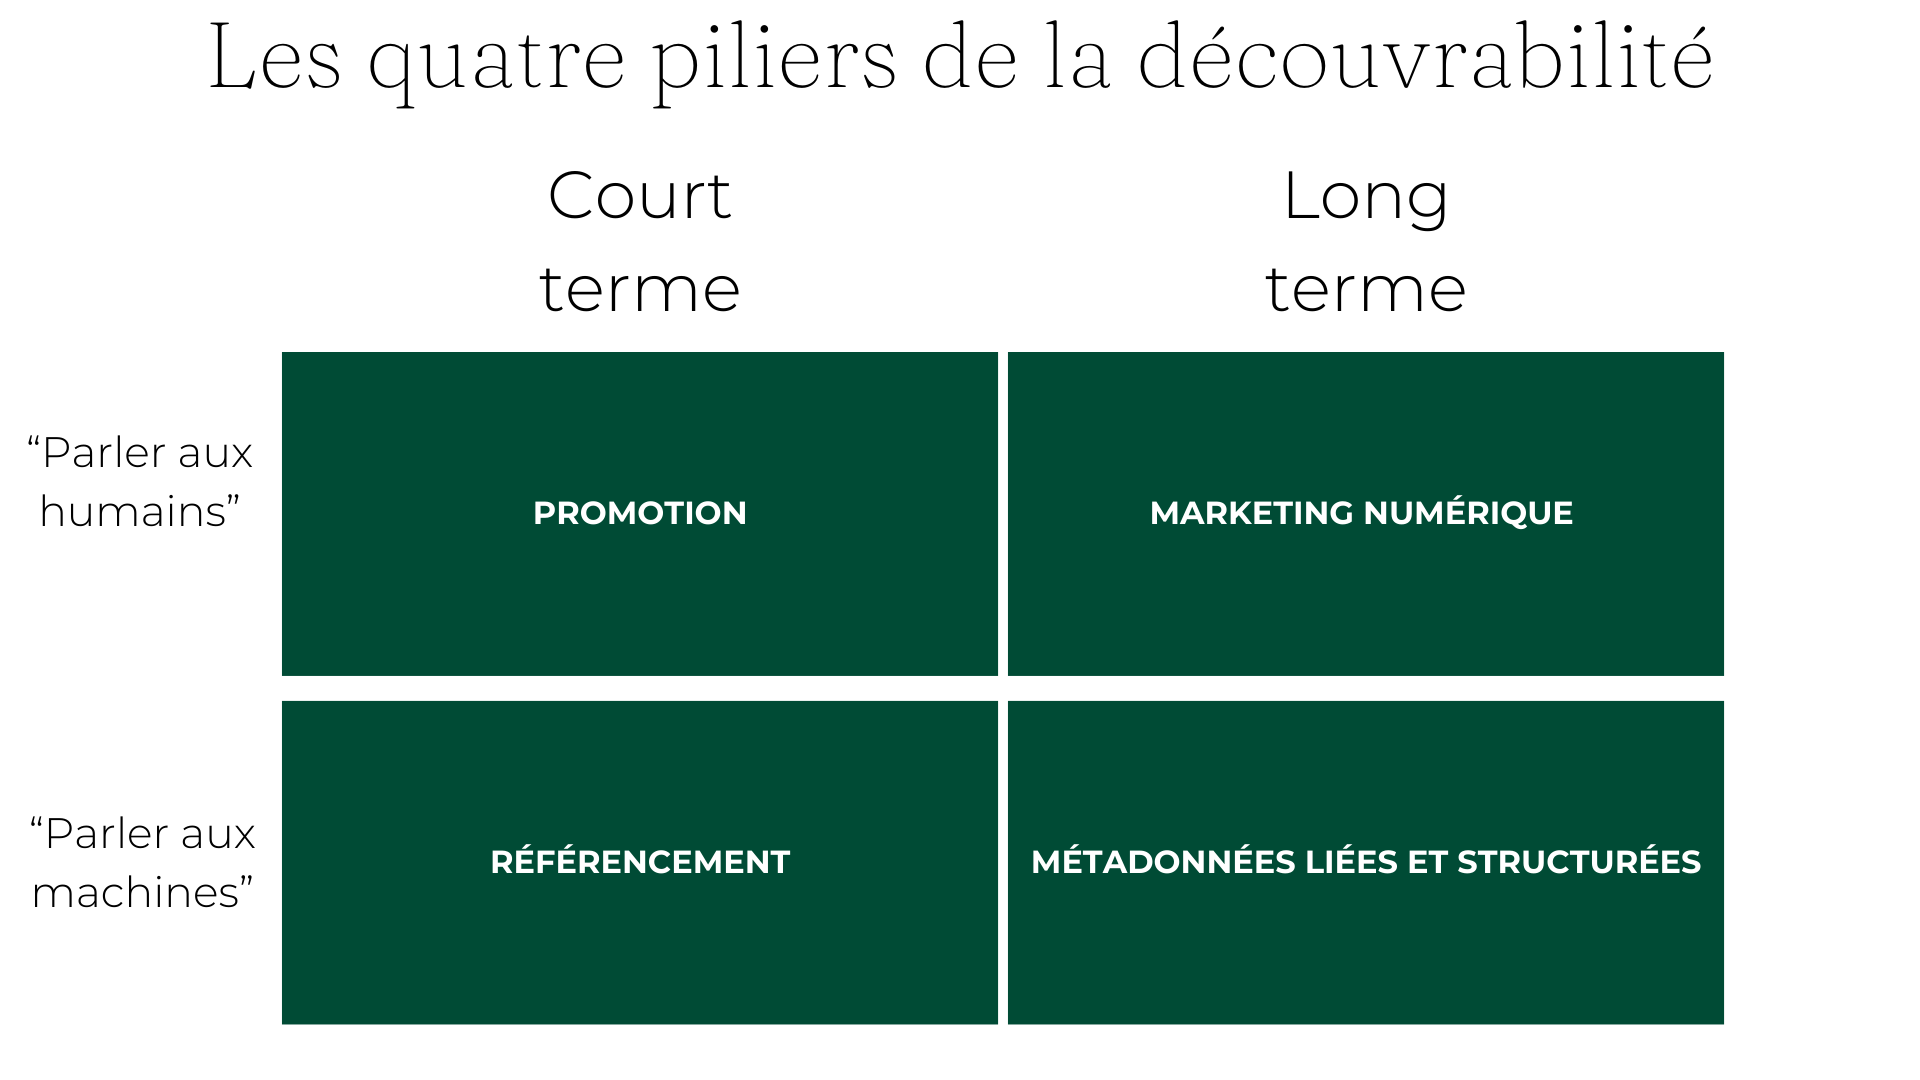
\includegraphics[width=0.8\textwidth]{images/image26.png}
	\caption{Les quatre piliers de la découvrabiltié}
	\label{fig:image26}
\end{figure}



Il y a donc un manque de formation des professionnels de la culture aux enjeux de découvrabilité qui est parfois compensée par ces derniers qui ont à leur disposition en ligne des formations gratuites souvent proposées par les GAFAMS\footnote{Google Apple Facebook Amazon Microsoft }, ce qui pose non seulement la question de la dépendance à ces outils, mais aussi celle de la pertinence de telles formations, pas toujours adaptées aux cas d’usages spécifiques des secteurs culturels.\footcite[p. 22]{ministeresdelaculturefranceetquebec2020} Évidemment, cette question de la formation est avant tout celle des moyens mis à disposition des institutions pour accomplir leurs missions, car il faut des professionnels qualifiés pour les remplir et donc de l’argent pour les recruter. Par ailleurs, la stratégie de promotion des contenus culturels passe parfois par l’achat d’espaces publicitaires en ligne ou la mise en place de partenariats, par exemple avec des influenceurs dont le rapport note l’importance croissante.\footcite[p. 22]{ministeresdelaculturefranceetquebec2020} 

Il faut aussi noter un frein simplement mentionné dans le rapport : celui de pratiques professionnelles qui \enquote{méritent d’être reconnues}.\footcite[p. 21]{ministeresdelaculturefranceetquebec2020} De fait, ces dernières et plus généralement le domaine du numérique, à cause de la complexité d’appréhension de leurs effets, parfois obscurs (d’où l’importance de l’explicabilité du code et de ses effets qui sera l’objet de la partie juste après) surtout dans le cas de la recommandation\index{Recommandation}, sont souvent assez mal vues et mal perçues par les institutions patrimoniales et leurs usagers. En témoigne le fait que la seule institution patrimoniale lauréate de l’appel à projets pour la découvrabilité en ligne des contenus culturels proposé par le ministère de la Culture soit le projet, déjà cité, data.bnf.fr\footcite{noauthor_decouvrabilite_2024}; et même s’il est vrai que l’institution est une tête de réseau qui fédère bon nombre d’acteurs au travers notamment du catalogue\index{Catalogue} collectif de France ou de Gallica (tous deux moissonnés par data.bnf.fr). D’autres acteurs du secteur patrimonial pourraient bénéficier de ces moyens pour améliorer la découvrabilité de leurs contenus culturels et notamment les musées.  

Il faut toutefois prendre en compte, qu’il est difficile voire impossible pour les institutions culturelles de rivaliser avec les moyens des GAFAMS en matière de découvrabilité de leurs contenus (par exemple Netflix investit 3 milliards par an rien qu’en marketing digital)\footcite[p. 23]{ministeresdelaculturefranceetquebec2020}, cependant, ces dernières ont des atouts qu’il ne faut pas négliger en la matière : la confiance des utilisateurs à leur égard bien sûr, mais aussi la possibilité de voir des régulations mises en place pour les favoriser, elles seront l’objet de notre prochaine partie.


\subsection{Règlementer pour favoriser la découvrabilité}

La question des régulations dans le domaine de la découvrabilité des contenus culturels est complexe et souvent négligée. Bien qu’ils ne constituent pas une solution universelle, certains ajustements règlementaires pourraient effectivement améliorer la visibilité des contenus culturels en ligne. Certains secteurs tels que la \textit{musique} et le \textit{cinéma} ont rapidement vu des règlementations sous forme de quotas être mises en place, tel est le cas par exemple de la loi Toubon qui a été votée en 1994 et qui impose aux radios de réserver une part variable (entre 40 et 10 \%) à la chanson française et aux artistes émergents\footcite{noauthor_comprendre_2016}. Plus récemment, le législateur européen s’est emparé de la question (directive services de \textit{médias audiovisuels}, traduite en 2021 en droit français) en demandant aux \textit{médias à la demande} de promouvoir les œuvres européennes en \enquote{facilitant l’accès à celles-ci} notamment, propose le texte, en les mettant sur la page d’accueil et en permettant aux utilisateurs de filtrer les œuvres européennes\footcite{noauthor_directive_2019}. Ce texte s’attaque donc directement à l’enjeu de découvrabilité en imposant, en plus des quotas, de réserver une place facilement repérable aux contenus européens. Ce type de réglementation de marché, assez classique, doit être complété, selon Mira Bruni (dans un rapport sur la diversités des contenus à l'ère numérique) d'une réglementation par les algorithmes, c'est-à-dire \enquote{des interventions ciblées avec des outils qui favoriseraient l'exposition à la diversité des contenus en augmentant la visibilité et la découvrabilité de certains types de contenus au moyen de processus éditoriaux effectués par les algorithmes.}\footcite{canadien2019}. Son propos est complété par M. Napoli qui indique qu'il est important de réglementer \enquote{l'intégration verticale}\footnote{L'intégration verticale est un concept dans lequel une entreprise contrôle plusieurs partie du processus économique, par exemple, dans notre cas : Netflix est à la fois producteur de contenus mais aussi diffuseur par le biais de sa plateforme, favorisant ainsi, algorithmiquement, les contenus produits  en propre. - Wikipédia, intégration verticale, consulté le 25/08/2024} dans le secteur culturel, car cette dernière favoriserait trop les contenus produits en propre par les plateformes. Par ailleurs, selon les auteurs du rapport cité plus haut, \enquote{l'autorégulation des plateformes en ligne a révélé ses limites}, il faut donc que les gouvernements aillent plus loin que l'incitation à la régulation\index{Régulation} et viennent directement réguler les plateformes, espaces privés dans la sphère publique qu'est le web ayant leurs propres règles.\footcite{canadien2019}.  

Si les secteurs cités plus hauts, parfois qualifiés de privilégiés, bénéficient d’un encadrement législatif fort qui tend à préserver la diversité culturelle (même si elle n’est que relative puisqu’elle veut surtout soutenir les productions nationales) ; ce n’est pas le cas pour tous. C’est assez logique dans le cas patrimonial où l’objectif est plutôt, on l’a déjà largement décrit, de briser les frontières entre les collections pour permettre leur diffusion à une large échelle, mais il faut tout de même noter que — et c’est plus une question de moyens financiers que de régulations — des institutions de petite taille voient le patrimoine qu’elles conservent invisibilisé par les \enquote{\textit{superstar}} que sont les grandes institutions, souvent parisiennes pour le cas de la France. La réglementation qui pourrait favoriser la visibilité et la découvrabilité des contenus de toutes les institutions serait plutôt sous forme de programmes d'aide à la numérisation, comme le plan de numérisation qui était au départ sous forme d'appels à projets annuels proposés par l'administration centralisée et qui a été déconcentré en 2018 dans les Directions régionales des affaires culturelles (DRAC) afin de cibler les institutions en région, plus en retard dans les chantiers de numérisation que les institutions centrales.\footcite{zotero-686} On peut aussi noter le Plan d'action pour le patrimoine écrit (PAPE) coordonné par la BnF et les pôles régionaux de coopération des acteurs du livre et de la lecture et région (par exemple Mobilis pour la région Pays-de-la-Loire)qui vise au signalement \enquote{des collections patrimoniales : manuscrits et archives sans limitation de date, livres imprimés jusqu’en 1830 pour l’ensemble des bibliothèques territoriales, livres imprimés jusqu’en 1914 pour les bibliothèques territoriales classées ou relevant d’une collectivité de plus de 500 000 habitants, fonds locaux et spécialisés, sans limitation de date.}\footcite{zotero-688}. Tous les ouvrages signalés ainsi sont intégrés au catalogue\index{Catalogue} collectif de France (CCFr), hébergé par la BnF, qui rassemble ainsi en un point d'entrée unique des collections éparpillées sur tout le territoire, permettant à des bibliothèques de taille très modeste d'avoir une visibilité à l'échelle nationale. 

\subsection{La question des droits d'auteurs}

Concentrons-nous dans cette partie sur une règlementation absolument centrale en ce qui concerne la découvrabilité des contenus patrimoniaux : le droit d’auteur\index{Droit d’auteur}. Car comme le rappelle très bien le rapport sur la découvrabilité déjà cité, \enquote{Vecteur indispensable de découvrabilité en ligne, les images sont, pour certains secteurs (\textit{arts visuels} et \textit{patrimoine}), souvent protégés par des droits d’auteur qui en empêchent l’exploitation en ligne, à moins de disposer de budgets considérables pour lever ces droits, ou d’une meilleure répartition de la valeur issue de l’exploitation de ces images par les plateformes. C’est un enjeu devenu encore plus névralgique depuis que Google propose toujours plus d’images dans les résultats de recherche pour tenir compte de cette préférence des utilisateurs}\footcite[p. 32]{ministeresdelaculturefranceetquebec2020}.

Rappelons donc ici le cadre légal actuel brièvement (il concerne toute l’Union européenne, on parle de droit continental). Le droit d’auteur\index{Droit d’auteur} est divisé en deux parts : les droits moraux d’abord, qui sont perpétuels, inaliénables et imprescriptibles et qui incluent le droit de paternité (l’auteur d’une œuvre sera toujours reconnu comme tel) et le droit au respect de l’œuvre (qui la protège contre toute modification susceptible de la dénaturer) ; les droits patrimoniaux quant à eux permettent à l’auteur de tirer des revenus de son œuvre, ils incluent le droit de reproduction (copie de l’œuvre) et de représentation (visibilité publique de l’œuvre), en France ils durent 70 ans sauf à de rares exceptions (notamment pour les auteurs morts pour la France)\footcite{zotero-323}. Cet arsenal législatif est complété par la directive européenne sur le droit d’auteur\index{Droit d’auteur} et les droits voisins dans le \textit{marché unique numérique} (adoptée en 2019 et transposée en droit français en 2021), qui renforce ces protections. Cette directive introduit des mécanismes pour que les créateurs soient équitablement rémunérés pour l’exploitation de leurs œuvres en ligne, en particulier lorsqu’elles sont utilisées par des plateformes comme \textit{YouTube} ou \textit{Google}\footcite{noauthor_directive_2019}. 

Maintenant que le cadre est posé, il faut noter quelques éléments importants. Premièrement, le droit d’auteur\index{Droit d’auteur} actuel constitue une limitation assez importante dans la disponibilité\index{Disponibilité} des collections culturelles en ligne, et notamment pour les musées d’art contemporain à l’image du \textit{Centre Pompidou} qui a numérisé et mis en ligne une grande partie de sa collection et a pour cela dû faire un nombre très important de demandes d’autorisations, car la majeure partie des œuvres étaient encore protégées par le droit d’auteur\index{Droit d’auteur}\footcite[§ 10]{bermes_parcours_2013}. Si le musée a pu \enquote{se permettre} humainement de faire toutes ces demandes, ce n’est pas le cas de toutes les institutions qui n’ont parfois que peu de personnel à leur disposition et qui doivent déjà faire face à des coûts de numérisation parfois (très) élevés. Pourquoi ne pas alors étendre la directive européenne citée plus haut pour que les plateformes visées paient une contribution, finalement assez logique, aux institutions patrimoniales dont elles diffusent les données afin que cela contribue aux frais de numérisation et de maintenance ? C’est d’ailleurs ce que fait Google avec \textit{Wikipédia} en finançant l’association en échange d’un accès plus facile et perfectionné à la base de données \enquote{\textit{Wikidata}}\footcite{noauthor_google_nodate}. 

Pour finir sur la question des règlementations, il faut aussi noter que les institutions ont souvent tendance à elles-mêmes s’en imposer et sont assez frileuses contrairement aux grands groupes. À l’image de Google qui, à travers son projet \textit{Google Books}, a tenté de contourner les lois sur le droit d’auteur\index{Droit d’auteur}, notamment en ce qui concerne les œuvres orphelines qui sont des œuvres pour lesquelles le ou les détenteurs des droits d’auteur ne peuvent pas être identifiés ou retrouvés, rendant ainsi toute exploitation légale complexe. Google, en numérisant massivement des livres sans avoir toujours obtenu l’accord des titulaires des droits et en supposant, par défaut, que les ayants droit étaient d’accord pour voir leurs œuvres diffusées, charge pour eux d’indiquer le contraire (on parle d’OPT-OUT). Cependant, cette approche a rapidement rencontré une opposition farouche, notamment de la part des auteurs et des éditeurs qui voyaient dans cette démarche une atteinte directe à leurs droits. La justice américaine a fini par trancher en 2011, estimant que Google ne pouvait pas se permettre de publier ces œuvres sans un accord préalable\footcite{ertzscheid2019}. Quel que soit le résultat, cet exemple illustre bien comment une entreprise de la taille de Google a tenté de \enquote{jouer} avec les lois existantes, dans l’espoir de créer un précédent favorable pour ses intérêts. Pour sortir d’une posture manichéenne où Google serait le \enquote{méchant}, il faut tout de même noter que si l’entreprise avait gagné ce procès cela aurait été une formidable opportunité de diffusion d’œuvres qui jusque-là étaient totalement introuvables en plus, évidemment, de générer des revenus très importants à l’entreprise américaine. Un autre exemple montre bien qu’il faut nuancer cela, c’est celui d’un autre procès opposant \textit{Internet Archive} (fondation archivant le \textit{web}) et quatre grands éditeurs internationaux (\textit{Hachette}, \textit{HarperCollins}, \textit{John Wiley \& Sons} et \textit{Penguin Random House}) qui a débuté en 2020, les éditeurs accusant la fondation de diffuser des livres sans respecter le droit d’auteur\index{Droit d’auteur}. Car la fondation effectue des sauvegardes de la quasi-totalité des sites \textit{internet} depuis sa création, mais aussi des copies de livres et en 2020, elle avait mis en place un service de prêt gratuit (pendant la pandémie et la fermeture des bibliothèques) sans limites d’utilisateurs simultanés pouvant emprunter les ouvrages. Pour les éditeurs : il s’agit purement et simplement d’un piratage de masse là où la fondation argue du fait qu’elle respecte le droit d’auteur\index{Droit d’auteur} en restant dans un \enquote{\textit{fair use}} (usage raisonnable, notion de droit américain qui prévoit des exceptions au droit d’auteur\index{Droit d’auteur} pour faciliter la diffusion des idées)\footcite{noauthor_aux_2023}. Au final, \textit{Internet Archive} a perdu ce procès et a donc dû retirer ces livres de sa bibliothèque\footcite{noauthor_condamnee_nodate}.

Si ces deux exemples peuvent tout à fait justifier la peur qu’ont les institutions de \enquote{jouer} avec les règlementations, on peut tout de même parfois se désoler de leur pusillanimité en la matière, et même si, par définition, il est difficile de trouver des exemples de projets avortés par des institutions du fait de leur frilosité, on peut tout de même prendre un exemple vécu pendant notre stage. Nous avions noté que la carte interactive des contenus présentée en partie 2 était un excellent moyen de valoriser les collections de la RTS en ligne, car souvent la première recherche que l’on effectue est simplement le nom de notre commune de naissance, mais on nous a beaucoup dit — et à raison sûrement — qu’il n’était pas envisageable de la rendre accessible au public, car cela pourrait poser des problèmes pour l’institution, car cela risquait de rendre visible le fait que la majorité des sujets diffusés par la RTS concernaient les cantons de Genève et de Vaud, ce qui est assez logique compte tenu de la population de ces deux cantons (qui plus est, le canton du Jura n’est indépendant que depuis 1978 et n’existait pas avant cette date), mais par peur d’une réaction négative des auditeurs, dans un contexte assez tendu pour la RTS (qui devra faire face à une votation qui vise à réduire la redevance à 200 francs en 2025). Il est vrai que donner une vision d’ensemble des collections n’est donc pas forcément une bonne chose politiquement, car cela renseigne sur les pratiques de conservation. Mais tout de même, si l’on avait pris le temps de l’explication et de la justification, le public aurait sûrement très bien compris cette sur-représentation de certains territoires et l’outil aurait pu être très utile. Notons aussi, sans disposer d’informations précises sur le sujet, que le projet \textit{data.ina.fr} qui vise à proposer des statistiques sur les contenus conservés par l’institution qui devait être lancée en juin de cette année\footnote{C'est en tout cas ce qui a été annoncé lors d'une visite à l'INA en janvier dernier} ne l’est toujours pas : peut-être pour des raisons similaires à celles évoquées pour la RTS ? L’explication du fonctionnement des algorithmes et outils, surtout avec l’émergence des outils d’intelligence artificielle\index{Intelligence artificielle}, revêt donc une importance capitale. Mais est-ce que la notion de découvrabilité peut aussi s’appliquer à découvrir de façon pertinente le fonctionnement des algorithmes et du code en général ? Ce sera l’objet de notre prochaine partie.


\chapter{Les angles morts de la notion de découvrabilité}

\subsection{Découvrabilité appliquée au code : l'explicabilité}

Dans sa revue des cinq grands enjeux de l’intelligence artificielle\index{Intelligence artificielle}, le journal \enquote{Polytechnique insight} note l’importance de \enquote{justifier les décisions prises par un algorithme}\footcite{noauthor_nouveaux_nodate}, ce qu’on peut tout à fait rapprocher de la notion d’explicabilité du code qui se définit comme suit : \enquote{capacité de mettre en relation et de rendre compréhensible les éléments pris en compte par le système pour la production d’un résultat.}\footcite{zotero-315}. Cette notion prend une importance croissante avec le développement de l’intelligence artificielle\index{Intelligence artificielle}, en témoigne le rapport Villani (2018) français et son intégration à la stratégie européenne en matière d’intelligence artificielle\index{Intelligence artificielle}\footcite[p. 14]{maxwell_comment_2020}. La notion est d’ailleurs existante dans le droit français, les algorithmes de service public déjà évoqués sont en effet, au même titre que les agents, redevables de leurs actions. \enquote{Les administrations qui conçoivent et utilisent des algorithmes publics doivent donc “rendre des comptes” de leur utilisation auprès des individus concernés, mais aussi de la société dans son ensemble.}\footcite{noauthor_algorithmes_nodate-1}. 

Le rapport \enquote{Flexible and Context-Specific AI Explainability: A Multidisciplinary Approach} écrit par Valérie Beaudouin, Isabelle Bloch \textit{et al.}\citein[p. 14]{beaudouin2020}{maxwell_comment_2020} distingue quatre facteurs d’explicabilité : le destinataire (utilisateur, régulateur, expert…) ; le niveau d’importance de l’algorithme (besoins différents entre expliquer les raisons d’un crash de voiture autonome et les résultats de Google) ; le cadre légal et l’environnement de déploiement (application critique, besoin d’un usage facilité au maximum, etc.). Isabelle Bloch, titulaire de la chaire en intelligence artificielle\index{Intelligence artificielle} de Sorbonne université, note (propos recueillis par Sophy Caulier)\footcite{noauthor_nouveaux_nodate} à ce propos : \enquote{Je travaille, par exemple, avec des médecins-radiologues sur la mesure de l’épaisseur du corps calleux chez les prématurés. Les radiologues voulaient savoir d’où venaient les scores obtenus, quelle région avait été reconnue dans l’image, où avaient été faites les mesures, pour comprendre ce qui avait contribué à la décision et expliquer le résultat final. Ces étapes étaient nécessaires pour qu’ils aient confiance dans l’outil.}

De la même façon, dans le cas patrimonial, un chercheur souhaitant écrire un article sur l’iconographie de Clytemnestre dans \textit{Gallica} souhaitera savoir pourquoi et comment le RAG\index{Intelligence artificielle!RAG} fonctionne pour identifier les éventuelles lacunes et biais (par exemple l’oubli d’un vase grec où elle n’est représentée que de façon incertaine) ; une personne cherchant simplement à consulter une image de la femme d’Agamemnon sera satisfaite du résultat sans avoir besoin de comprendre ses tenants et aboutissants. Cette problématique d’identification : parmi des milliards de paramètres et de documents, celui qui aura influencé le résultat d’une requête ou d’une recommandation\index{Recommandation} rejoint totalement celle posée depuis le début de ce mémoire autour de la notion de découvrabilité. Dans les deux cas, le niveau d’explicabilité requis va dépendre des quatre facteurs cités plus haut. 

L’explicabilité est l’un des enjeux pris en compte dans le projet \textit{Archival}, qui vise à poser la question du rôle de l’intelligence artificielle\index{Intelligence artificielle} dans l’interprétation de fonds d’archives\citein{noauthor_valorisation_nodate}{2023e} et dont le principe est de créer une interface\index{Interface} de résultats alimentée par l’intelligence artificielle\index{Intelligence artificielle} qui, en plus des résultats à proprement parler, donnerait à voir le processus de génération\footcite[p. 46]{besnehard_evaluer_nodate}. Cinq algorithmes sont mis à disposition du chercheur qui devra sélectionner celui adapté à son cas d’usage, ils sont vus comme \enquote{les outils de la suite bureautique}\footcite[p. 9]{agnola_ia_2022} choisis par les utilisateurs en connaissant leurs fonctionnements et leurs avantages. 


\begin{figure}[h!]
	\centering
	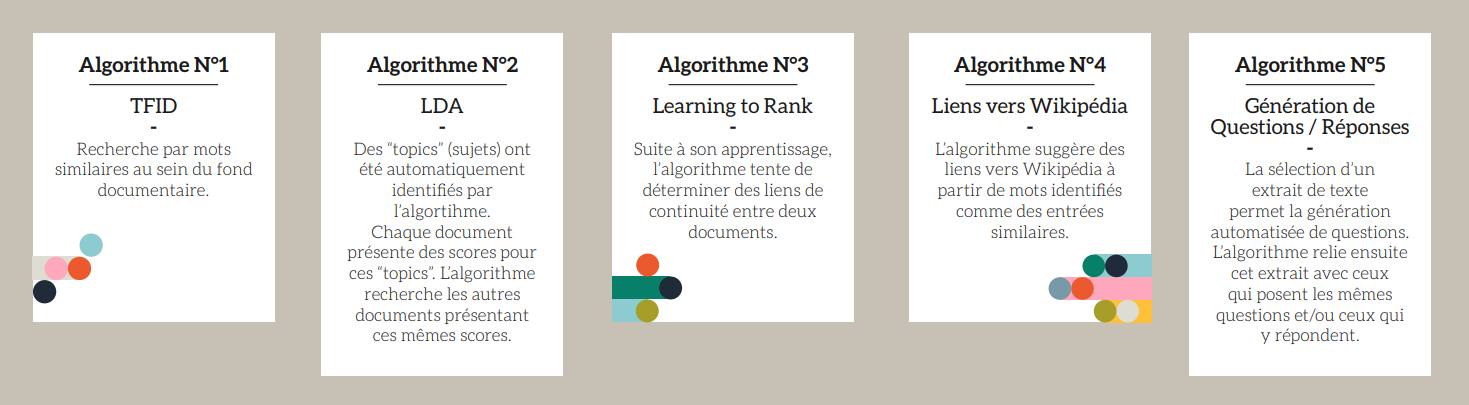
\includegraphics[width=0.8\textwidth]{images/image27.png}
	\caption{Les différents algorithmes à l'oeuvre dans \textit{Archival}}
	\label{fig:image27}
\end{figure}

\begin{center}
	Depuis : Agnola, Azémard, de Silva
\end{center}


L’approche est dite de la \enquote{boite transparente} (\textit{glass box})\footnote{Par opposition à l’effet boite noire (black box) souvent décrit pour évoquer la difficulté de compréhension des processus liés à l’intelligence artificielle\index{Intelligence artificielle}.}, dans laquelle l’enjeu n’est plus uniquement le résultat, mais le processus qui y mène\footcite[p. 47]{besnehard_evaluer_nodate}. L’objectif pour l’équipe du projet est d’expliquer en détail ce que fait chaque algorithme pour que les usagers comprennent les biais et problématiques posées ; de même qu’on a appris que pour trouver le journal \enquote{le voleur} dans un moteur de recherche il fallait, pour éviter les problématiques d’homonymie ajouter \enquote{journal} à notre requête, les chercheurs auront à apprendre les biais et problématiques de l’intelligence artificielle\index{Intelligence artificielle} grâce à une démarche d’explicabilité des projets. Cette notion est donc autant du côté des producteurs et des créateurs d’interfaces qui doivent les rendre les plus transparentes possibles que du côté des utilisateurs qui doivent s’acculturer au numérique et comprendre ses écueils. On a là un exemple d’explicabilité dite globale, c’est-à-dire que ce qui est donné à comprendre à l’usager est le fonctionnement général de l’algorithme, à la différence du niveau local où on expliquerait chacune des décisions que ce dernier prendra\footcite[p. 15]{maxwell_comment_2020}.

\subsection{L'accessibilité numérique}

Dans le rapport sur la découvrabilité en ligne des contenus culturels francophones, déjà cité plusieurs fois, qui est l’illustration des politiques culturelles mises en œuvre pour l’amélioration de cette dernière. Une notion est presque totalement absente : l’accessibilité\index{Accessibilité} numérique. Elle n’est mentionnée qu’une seule fois à la page 25 : \enquote{Par ailleurs, les métadonnées renseignant les fonctionnalités d’accessibilité\index{Accessibilité} disponibles avec le contenu (par exemple, une composante d’audiodescription associée à une vidéo) sont essentielles pour la découvrabilité de ces contenus auprès des personnes en situation de handicap (mental, auditif, visuel, moteur, etc.).} Si ce qui est écrit est tout à fait vrai, il nous semble que c’est une vision un peu restrictive de la question des métadonnées d’accessibilité\index{Accessibilité} et de leur intérêt pour la découvrabilité. Mais avant de poursuivre, prenons le temps de définir ce qu’est l’accessibilité\index{Accessibilité} numérique et ce que cela implique. Selon \enquote{mon parcours handicap}, site d’information pour les personnes en situation de handicap et leurs aidants, l’accessibilité\index{Accessibilité} numérique c’est ce qui permet aux personnes en situation de handicap d’accéder aux contenus d’un site web sans difficulté\footcite{noauthor_accessibilite_nodate}. Cela implique donc quatre notions importantes : la perception par tous les publics (textes alternatifs aux contenus non textuels par exemple) ; l’utilisation (navigation simple et \enquote{logique} pour trouver le contenu même sans le voir) ; la compréhension (création de pages prévisibles, aides à la saisie) et la robustesse (optimisation de la compatibilité)\footcite{noauthor_notion_nodate}. L’accessibilité\index{Accessibilité} ce n’est donc pas simplement le fait de rajouter des textes de remplacements aux images sur un site, c’est un processus qui doit être abordé depuis le design du projet et pendant toute sa durée de vie\footcite{noauthor_accessibilite_nodate} pour prendre en compte tous les publics. Alors qu’entre 4,3 \% et 13,8 \% de la population sont considérés comme handicapés en France (selon le degré de handicap pris en compte, les nombres sont très différents), soit entre 2.8 et 9 millions de personnes\footcite{noauthor_personnes_2022}. Une politique de découvrabilité ne peut donc se passer d’une politique d’accessibilité\index{Accessibilité}.

Loin d’être uniquement, comme on le lit souvent, une contrainte, l’accessibilité\index{Accessibilité} doit être vue comme une opportunité pour les créateurs de sites. Car avoir une démarche de mise en accessibilité\index{Accessibilité} d’un site les oblige à poser la question de sa navigation qui doit être la plus simple et la plus logique possible pour que, notamment, les lecteurs d’écran ne s’y perdent pas. Or, un lecteur d’écran fonctionne exactement de la même manière qu’un \textit{crawler}, ces petits robots qui parcourent automatiquement les sites web pour les indexer afin que les moteurs de recherche puissent les afficher. Plus un site est clair, sa navigation fluide et aisée, mieux le lecteur d’écran pourra le lire et mieux le \textit{crawler} en comprendra la structure, le plan donc meilleure sera l’indexation de votre site et donc son référencement\index{Référencement} et sa repérabilité\index{Repérabilité} sera accrue\footcite{adminat_et_2023}. Par ailleurs, le fait de renseigner les fameux textes de remplacement sur les images permet aussi aux moteurs de recherche de les indexer, et donc de les afficher, améliorant ainsi le référencement\index{Référencement} de ces dernières.

Autre notion importante, rendre un site accessible c’est-à-dire souvent plus clair et plus facile dans sa navigation est aussi utile pour une catégorie de gens souvent oubliés : ceux souffrant de ce qu’on appelle la fracture numérique ou l’illectronisme, qui toucherait plus de 15 \% de la population française en 2021\footnote{Selon des chiffres de l'INSEE \url{https://www.insee.fr/fr/statistiques/7633654}}. Donc, la mise en accessibilité\index{Accessibilité} permet aussi à ces publics qui ont des difficultés à comprendre l’univers numérique de naviguer et d’utiliser plus facilement les sites. Dernier élément à prendre en compte, l’accessibilité\index{Accessibilité} doit aussi se placer du côté des machines et des connexions \textit{internet} : un site web accessible doit donc améliorer son temps de chargement (ce qui améliore aussi son référencement\index{Référencement}), ce qui en plus de le rendre plus facilement consultable pour tous permet d’économiser des ressources matérielles et informatiques et donc de réduire l’impact carbone, grandissant du numérique qui sera l’objet de notre prochaine partie.

\subsection{Et la planète dans tout ça ?}

La fin de la loi de Moore est-elle un motif d’espoir ? C’est en tout cas ce qu’écrit Tristan Nitot, ex-président de Mozilla Europe et personnalité influente du monde du numérique\footcite{nitot_loi_2024}. Mais qu’est-ce que la loi de Moore et pourquoi serait-ce une bonne nouvelle que d’annoncer sa mort ? Formulée il y a bientôt 60 ans (1965) par le co-fondateur d’Intel Gordon Moore qui la résumait par cette phrase : \enquote{le nombre de transistors dans les semiconducteurs [les processeurs] va doubler tous les deux ans à coût constant}\footcite{zotero-301}. Si l’on veut résumer grossièrement, un transistor est une espèce d’interrupteur qui peut être commandé, plus ils sont nombreux plus un processeur peut faire de calculs, puisqu’ils sont responsables de ces derniers : les 0 et 1 du binaire étant en fait l’état des transistors selon qu’ils sont éteints ou allumés\footcite{2024e}. Si la loi de Moore se vérifie toujours si on regarde le nombre de transistors, actuellement de 50 milliards dans nos processeurs, en observant plutôt la puissance de calcul, elle ne se vérifie plus, car si le nombre de transistors est effectivement relié à cette variable, d’autres paramètres entrent en ligne de compte.

Au final, comme l’écrit l’auteur, cela peut devenir un motif d’optimisme. Car le corollaire de la loi de Moore, la loi de Wirth, qui se résume elle aussi en une phrase \enquote{ce qu’Intel vous donne, Microsoft le reprend} qui nous montre que l’augmentation de puissance des processeurs qui s’est observée depuis des années s’est toujours accompagnée d’un ralentissement de nos applications et pages web qui sont, par exemple, 150 fois plus lourdes qu’il y a 25 ans\footcite[§ 8]{nitot_loi_2024}. Par ailleurs, si la loi de Moore stipulait que le coût devait rester constant, ce n’est plus vraiment le cas, les consommations étant en constante augmentation de même que les prix\footcite[§ 4- § 6]{nitot_loi_2024}. On avait donc une fuite en avant avec des processeurs qui devenaient de plus en plus puissants avec des applications de plus en plus gourmandes : ce n’était évidemment pas soutenable scientifiquement parlant (la réduction des tailles de transistors ayant tout de même des limites de même que leur refroidissement qui est le principal problème aujourd’hui), mais aussi écologiquement parlant. On préférait toujours développer des fonctionnalités supplémentaires à des applications, sans jamais prendre le temps de les optimiser, ces dernières étaient donc de plus en plus lourdes et de moins en moins optimisées, ce qui était possible avec la loi de Moore ne le sera plus bientôt\footcite[§ 9]{nitot_loi_2024}. Ce faisant, nos ordinateurs personnels, qui étaient avant constamment ralentis et mis au ban, car trop peu performants, pourraient dans le futur être plus durables avec la fin de la loi de Moore.

Quand on note que 90 \% de l’impact carbone du numérique était causé en 2021 par son cycle de fabrication, qui en plus nécessite des matériaux rares, extraits souvent dans des conditions inhumaines\footcite[§ 16]{guillard_chapitre_2021} : on peut se dire, et à raison, que la conservation de nos terminaux personnels le plus longtemps possible est essentielle. Quant au reste de l’impact carbone du secteur, il est lié à son usage, et 80 \% sont le fait du visionnage de vidéos. Il ne faut donc pas éluder cette question de l’usage, car, par ailleurs, entre 2021 et 2024, la tendance est en train de s’inverser avec un impact carbone de 78 \% du côté de la fabrication et de 22 \% du côté de la phase d’utilisation\footcite{noauthor_quelle_nodate}. Les causes ? L’explosion de l’usage de la vidéo à la demande et du média sur les réseaux sociaux (penser à \textit{Tik Tok} par exemple) d’une part, et de l’autre — et on l’avait simplement évoqué dans notre partie 1 — l’impact grandissant de l’intelligence artificielle\index{Intelligence artificielle} générative. Ces dernières, et leurs milliards de paramètres (1000 milliards dans GPT-4\footnote{Selon les estimation les plus probables (\textit{in} Wikipédia, GPT-4)}) consomment des quantités d’énergie extrêmement importantes, car elles ont besoin d’une puissance de calcul immense pour fonctionner. C’est valable pendant leur phase d’entrainement, par exemple GPT-3 et ses 175 millions de paramètres a généré 552 tonnes d’équivalent CO2\footcite{noauthor_pourquoi_2023}, en sachant que si l’on se fie aux interprétations des Nations unies dans leur rapport \enquote{emission gap report 2020}\footnote{\textit{in} \url{ https://bonpote.com/objectif-2-tonnes-vrai-defi-ou-mauvaise-cible/}}, pour limiter le réchauffement à 1,5°C (et donc respecter l’accord de Paris pour le climat) nous devrions tous émettre environ 2 tonnes par an : cet entrainement (et encore d’un modèle ancien faute de données récentes) est donc loin d’être négligeable. C’est évidemment aussi valable pendant la phase d’utilisation (et sûrement bien plus) des modèles, et ici aussi les chiffres font défaut, on peut noter que Google a augmenté l’année dernière son empreinte carbone de 48 \% et Microsoft (qui héberge \textit{OpenAI}) de 39 \% (alors que les émissions du géant américain étaient en baisse depuis quelques années)\footcite{noauthor__nodate}. Quand on sait que les émissions mondiales du secteur représentaient 3,7 \% en 2021 et devraient représenter 9 \% d’ici à 2052, c’est-à-dire autant que les voitures, il ne faut pas négliger cet aspect, même dans une politique de découvrabilité. Car cette dernière a besoin, elle aussi, de beaucoup de données : pour générer les visualisations de données et interfaces nouvelles et généreuses vues dans la partie 2 par exemple, mais aussi pour stocker et rendre disponible au plus grand nombre le patrimoine numérisé. Il ne faut donc pas que les institutions fassent une \enquote{course en avant} dans le domaine et numérisent l’intégralité de leurs collections dans l’objectif de la faire découvrir en totalité, mais plutôt qu’elles le fassent — comme c’est plutôt le cas actuellement il faut le souligner — de façon raisonnée et sobre. \enquote{Combien faut-il numériser de missels du XIX\textsuperscript{e} siècle pour témoigner de la piété de la société à cette époque ?}\footcite[p. 21]{bermes2024}. Dans le cas du patrimoine audiovisuel par ailleurs, il faut aussi veiller à ne pas forcément proposer la qualité d’image maximale (déjà ça n’a pas toujours de sens au vu des conditions dans lesquelles étaient regardées les émissions de l’époque), mais plutôt l’adapter au support de lecture et à l’usage qui en sera fait.

% Import de la partie 3
	
	
	
	\chapter*{Conclusion}
	\addcontentsline{toc}{chapter}{Conclusion}
	
	
	À l'heure où s'achève cette réflexion, une nouvelle interrogation surgit : la découvrabilité, n'était-elle qu'un prétexte ? Tout au long de notre étude, nous avons présenté cette notion comme une réponse aux défis posés par ce que nous avons qualifié de big data patrimonial. Pourtant, il ne s'agit que d'un mot, un concept, loin d’être performatif. Bien que fréquemment invoqué pour résoudre les enjeux contemporains tels que les mégadonnées, la bataille de l'attention ou encore la fatigue muséale, la découvrabilité n’est qu’un prétexte, un point d'entrée pour aborder une multitude de problématiques sous-jacentes. Son émergence ne signale pas un problème nouveau, mais plutôt les possibilités qui s'offrent aux institutions pour y faire face.
	
	L’émergence des contenus culturels est ici la question centrale (définir la découvrabilité en note en indiquant que le mot est dedant).  
	Émergence au sein de nos moteurs de recherche, grâce à une double stratégie visant, en premier lieu, à « parler aux machines », par le biais des principes du web sémantique, mais aussi, dans un second temps, à « parler aux humains » en leur proposant du « contenu utile et de qualité ». Émergence au sein des plateformes, en provoquant une « sérendipité artificielle » par l’intermédiaire des algorithmes de recommandation. Émergence au sein des catalogues et que grâce à la visualisation de l’information émergent  de nouveaux questionnements, qu’ils soient intellectuels or organisationnels. Qu’ils émergent pour découvrir les collections patrimoniales sous un autre angle et en allant plus loin grâce à des interfaces devenues généreuses. En enfin, émergence active, guidés par l’intelligence artificielle, qui, telle Orphée et malgré des intentions bienveillantes finit par se retourner, égarant ainsi sa bien-aimée, le guide devenant ainsi la raison de la perte s’il est suivi aveuglément. 
	
	Corollaire de l’émergence, l’effacement : que devient ce qui n’a pas été rendu visible par les algorithmes, les interfaces ? Car l’émergence parmi un vaste ensemble conduit inévitablement à l’effacement, effacement de ce que les machines, le code, n’ont pas choisi de montrer. L’écosystème, le web, en tant qu’intercesseur vers le savoir et la découverte, se doit donc de rester impartial ; il aura alors atteint l’incroyable utopie numérique qu’il rendait possible à sa création. Mais en tant qu’écosystème de l’hyper : utopie de l’hyperchoix qui se transforme en une hyperindividualisation algorithmique ; utopie de l’hyperdiversité qui devient hyperstandardisation culturelle, l’hyperespace a grand besoin d’être pris en main par les acteurs patrimoniaux. Ces derniers doivent non seulement le comprendre et y être formés, mais ils doivent aussi être conscients de ses failles, sans tomber dans irrationnelle craintes qui limiterait les actions mises en place. Ils ont par ailleurs à leur disposition des moyens de lutte : la réglementation et leur réputation d’excellence.
	
	La découvrabilité doit donc prendre une place centrale dans les politiques culturelles, mais l’on doit garder à l’esprit qu’elle n’est qu’un prétexte. Ce que ce qui compte vraiment, c’est ce qu’elle sous-tend. Mais cette position névralgique ne doit pas faire oublier que même si la notion est à la croisée d’enjeux essentiels, elle doit en sortir en prenant des chemins alternatifs. Celui de l’accessibilité d’abord, qui doit être considérée comme une opportunité et non une contrainte : celle de rendre les contenus consultables par tous et celle d’être mieux repéré par les machines. Chemin nouveau, encore mal balisé, de l’intelligence artificielle ensuite ; dont on ne parvient pas toujours, tout comme Orphée, à expliquer les décisions qui nous mène au dernier chemin : celui de la viabilité écologique, que cette technologie, plus encore que les autres, vient mettre à mal.
	
	Concluons en revenant à Borges, dont l'œuvre a servi de point de départ à notre réflexion :
	
	\begin{quote} « La Bibliothèque est totale, et [...] ses étagères consignent toutes les combinaisons possibles des vingt et quelques symboles graphiques [...], c’est-à-dire tout ce qu’il est possible d’exprimer, dans toutes les langues. Tout : l’histoire minutieuse de l’avenir, les autobiographies des archanges, le catalogue fidèle de la Bibliothèque, des milliers et des milliers de catalogues mensongers, la démonstration de la fausseté de ces catalogues, la démonstration de la fausseté du catalogue véritable. »\footcite[p. 3]{borges1963} \end{quote}
	
	Borges avait saisi l'essence même de la découvrabilité : non seulement l'identification au sein d'une masse d'informations, mais aussi la question des régimes de vérité, qui se multiplient dans notre monde contemporain. L'enjeu de la découvrabilité est l'émergence d'un régime de vérité commun, vérifiable et explicable.
	
	Nous pensons, et c'est une forme d'hommage au vu du lieu de notre stage, que les médias publics ont un rôle crucial à jouer dans ce domaine. À l'instar des institutions patrimoniales, ils ne sont pas intrinsèquement biaisés, car ils ne sont pas soumis aux contraintes des logiques marchandes. Le code, c'est la loi ; veillons donc à ce qu'il nous permette de bâtir une société fondée sur des vérités partagées.
	
	\newpage{\pagestyle{empty}\cleardoublepage}
	
	\renewcommand\indexname{Index thématique (grandes notions)} % Index renommé 
	
	
	
	
	
	%%%%%%%%%%%%%%%%%%
	
	\appendix %Des appendices: tables figures, etc
	
	\chapter[Supports conservés]{}
	
	\begin{figure}[h!]
		\centering
		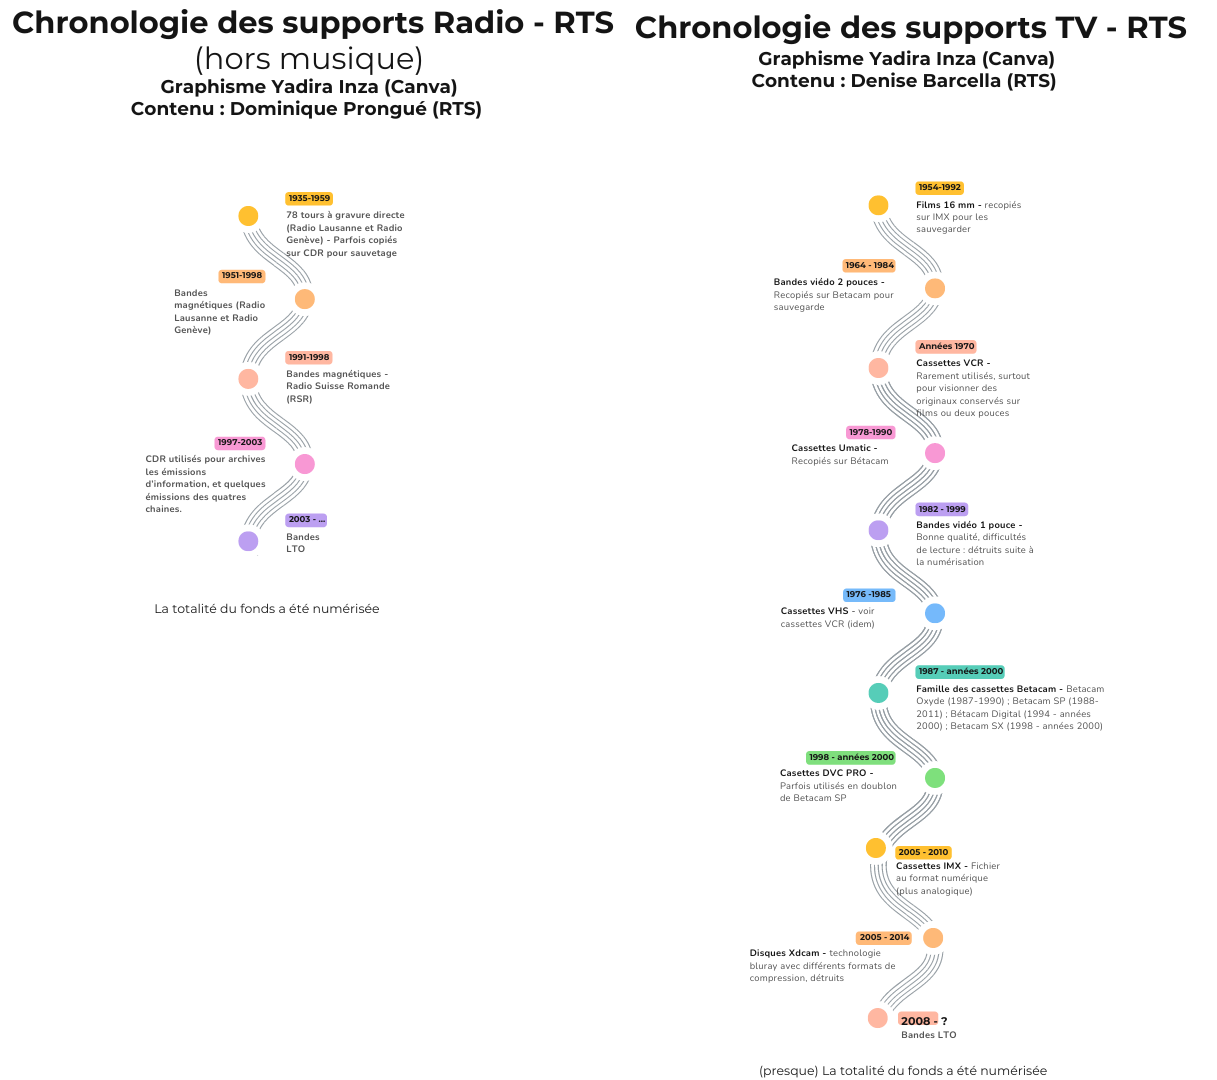
\includegraphics[width=1\textwidth]{images/supports_TVR_RTS.png}
		\label{fig:image27}
	\end{figure}
	
	
	\newpage{\pagestyle{empty}\cleardoublepage}
	
	%%%%%%%%%%%%%%%%%%
	
	\backmatter % glossaire, index, table des figures, table des matières.. (la bibliographie a déjà été appelée)
	
	\printindex

	\listoffigures
	\newpage % ajout d'une page pour séparer la liste des figures de la TOC
	\tableofcontents
\end{document}
